%----------------------------------------------------------------------------------------
%	PACKAGES AND OTHER DOCUMENT CONFIGURATIONS
%----------------------------------------------------------------------------------------

\documentclass{tufte-book} % Use the tufte-book class which in turn uses the tufte-common class
\setcounter{tocdepth}{3}
\setcounter{secnumdepth}{3}


\hypersetup{colorlinks} % Comment this line if you don't wish to have colored links

\usepackage{microtype} % Improves character and word spacing
\usepackage{isotope}
\usepackage{booktabs} % Better horizontal rules in tables


%%%%%%%%%%%%%%%%% PERSONAL ADDITIONS %%%%%%%%%%%%%%%%%

\usepackage{amsmath,amssymb,amsthm,cancel,physics,bm,simplewick,listings,longtable,relsize,amsfonts,pgfplots}

\usepackage[italian]{babel}

\usepackage[displaymath,textmath,sections,graphics,floats]{preview}
\usepackage{multirow}
\usetikzlibrary{intersections}
\usetikzlibrary{calc,patterns,angles,quotes}
\usepackage{tikz}
\usepackage{caption}
\usepackage{tikz-network}
\usepackage{float}
\floatplacement{figure}{H}
\pgfplotsset{compat = newest}

\theoremstyle{definition}
\newtheorem{definition}{Definition}

\theoremstyle{theorem}
\newtheorem{theorem}{Theorem}
\theoremstyle{plain}

\theoremstyle{remark}
\newtheorem*{remark}{Remark}

\theoremstyle{remark}
\newtheorem*{example}{Example}

% alias for planck constant
\newcommand{\hp}{\hslash}

% command to insert nuclear element \nucl{A}{Z}{elelement symbol}
\newcommand{\nucl}[3]{ \ensuremath{ \phantom{\ensuremath{^{#1}_{#2}}} \llap{\ensuremath{^{#1}}} \llap{\ensuremath{_{\rule{0pt}{.75em}#2}}} \mbox{#3} } }

\newcommand{\fraclarg}[2]{ \frac{ \mathlarger{#1} }{ \mathlarger{#2} } }

%% Real and Imaginary part of a complex number
\renewcommand{\Re}{\mathfrak{Re}}
\renewcommand{\Im}{\mathfrak{Im}}

%%%%%%%%%%%%%%%%%%%%%%%%%%%%%%%%%%%%%%%%%%%%%%%%


\usepackage{graphicx} % Needed to insert images into the document
\graphicspath{{graphics/}} % Sets the default location of pictures
\setkeys{Gin}{width=\linewidth,totalheight=\textheight,keepaspectratio} % Improves figure scaling

\usepackage{fancyvrb} % Allows customization of verbatim environments
\fvset{fontsize=\normalsize} % The font size of all verbatim text can be changed here

\newcommand{\hangp}[1]{\makebox[0pt][r]{(}#1\makebox[0pt][l]{)}} % New command to create parentheses around text in tables which take up no horizontal space - this improves column spacing
\newcommand{\hangstar}{\makebox[0pt][l]{*}} % New command to create asterisks in tables which take up no horizontal space - this improves column spacing

\usepackage{xspace} % Used for printing a trailing space better than using a tilde (~) using the \xspace command

\newcommand{\monthyear}{\ifcase\month\or January\or February\or March\or April\or May\or June\or July\or August\or September\or October\or November\or December\fi\space\number\year} % A command to print the current month and year

\newcommand{\openepigraph}[2]{ % This block sets up a command for printing an epigraph with 2 arguments - the quote and the author
\begin{fullwidth}
\sffamily\large
\begin{doublespace}
\noindent\allcaps{#1}\\ % The quote
\noindent\allcaps{#2} % The author
\end{doublespace}
\end{fullwidth}
}

\newcommand{\blankpage}{\newpage\hbox{}\thispagestyle{empty}\newpage} % Command to insert a blank page

\usepackage{makeidx}
\usepackage{xcolor}
\usepackage{hyperref} % Used to generate the index
\hypersetup{colorlinks=true,linkcolor=red}
%\makeindex % Generate the index which is printed at the end of the document

%----------------------------------------------------------------------------------------
%	BOOK META-INFORMATION
%----------------------------------------------------------------------------------------

\title{Appunti di\\Fisica Nucleare} % Title of the book

\author{Niccolò Zanotti} % Author

\publisher{Open source publisher} % Publisher

%----------------------------------------------------------------------------------------

\begin{document}

\frontmatter

%----------------------------------------------------------------------------------------
%	EPIGRAPH
%----------------------------------------------------------------------------------------

% \thispagestyle{empty}
% \openepigraph{Quotation 1}{Author, {\itshape Source}}
% \vfill
% \openepigraph{Quotation 2}{Author}
% \vfill
% \openepigraph{Quotation 3}{Author}

%----------------------------------------------------------------------------------------

\maketitle % Print the title page

%----------------------------------------------------------------------------------------
%	COPYRIGHT PAGE
%----------------------------------------------------------------------------------------

\newpage
\begin{fullwidth}
~\vfill
\thispagestyle{empty}
\setlength{\parindent}{0pt}
\setlength{\parskip}{\baselineskip}
Copyright \copyright\ \the\year\ \thanklessauthor

\par\smallcaps{Published by \thanklesspublisher}

\par\smallcaps{\url{https://github.com/Feyn-23/Fisica-nucleare-subnucleare}}

\par Licensed under the Apache License, Version 2.0 (the ``License'');
you may not use this file except in compliance with the License.
You may obtain a copy of the License at \url{http://www.apache.org/licenses/LICENSE-2.0}.
Unless required by applicable law or agreed to in writing, software
distributed under the License is distributed on an \smallcaps{``AS I'' BASIS,
WITHOUT WARRANTIES OR CONDITIONS OF ANY KIND}, either express or implied.
See the License for the specific language governing permissions and
limitations under the License.\index{license}

% \par\textit{First printing, \monthyear}
\end{fullwidth}

%----------------------------------------------------------------------------------------

\tableofcontents % Print the table of contents

%----------------------------------------------------------------------------------------

% \listoffigures % Print a list of figures

%----------------------------------------------------------------------------------------

% \listoftables % Print a list of tables

%----------------------------------------------------------------------------------------
%	DEDICATION PAGE
%----------------------------------------------------------------------------------------

\cleardoublepage
% ~\vfill
% \begin{doublespace}
% \noindent\fontsize{18}{22}\selectfont\itshape
% \nohyphenation
% Dedicated to my family and friends.
% \end{doublespace}
% \vfill
% \vfill


\cleardoublepage

%%%%%%%%%%%%%%%%%%%%%%%%%%%%%%%%%%%%%%%%%%%%%%%%%%%%%%%%%%%%%%%%%%%%%
\chapter{Fisica nucleare}\label{ch:fisica-nucleare}
       
\section{Le unità di misura della Fisica Nucleare e Subnucleare}
\label{sec:unita-di-misura}

La scelta della unità di misura è arbitraria ma, in accordo con i criteri che ispirano i moderni sistemi, soddisfa alcuni semplici requisiti di ordine generale:
\begin{itemize}
    \item  **l'unità deve essere connessa ad un fenomeno naturale ritenuto stabile ed invariabile nel tempo** piuttosto che ad un oggetto o manufatto particolare il quale potrebbe deteriorarsi o modificare le sue proprietà con il tempo;
    \item  **le unità non devono essere ridondanti** e devono costituire un sistema di grandezze fisiche irriducibili dette fondamentali dalle quali ottenere tutte le altre che invece vengono dette derivate;
    \item  **l'unità deve essere riproducibile in laboratorio con una relativa facilità** (in realtà è lavoro da professionisti quali sono i metrologi).

\end{itemize}

Un sistema di unità di misura più appropriato può essere costruito facendo riferimento alle costanti fisiche fondamentali che governano i fenomeni nucleari e subnucleari.
Accanto alle grandezze fondamentali, ogni area della fisica introduce anche specifiche costanti fisiche.
Queste possono essere sia dimensionali che adimensionali, riferirsi a specifiche classi di fenomeni - e dunque di rango locale - oppure valide per ogni fenomeno fisico e quindi di rango universale.
Mentre il valore numerico delle costanti dimensionali dipende dalla scelta del sistema di unità misura, quello delle costanti adimensionali ne è del tutto indipendente per cui si ritiene che siano dotate di un più profondo significato fisico anche se a tutt’oggi nessuna teoria è in grado di predirne il valore.
Fu Planck che propose di assumere come grandezze fisiche fonda- mentali le costanti fisiche universali introducendo i cosiddetti sistemi naturali di unità di misura.
Lo scopo di tali sistemi è quello di dedurre le appropriate scale di lunghezze, tempi, masse e temperature diret- tamente dai fenomeni naturali piuttosto che da convenzioni di natura metrologica.

La costruzione di un sistema di unità di misura le cui grandezze abbiano la scala appropriata per una certa classe di fenomeni richiede l'introduzione di specifici vincoli tra le grandezze fondamentali della descrizione macroscopica.
Ad esempio, dato che **i fenomeni nucleari e subnucleari sono al tempo stesso relativistici e quantistici** ciò significa che le velocità, ovvero i quozienti tra lunghezze e tempi saranno dell'ordine di c, mentre le azioni, cioè i prodotti delle energie per i tempi caratteristici saranno dell'ordine di $\hslash$.
Due costanti universali non sono però sufficienti per fissare la scala delle tre grandezze necessarie al Sistema Internazionale per descrivere la relatività e meccanica quantistica (L, T ed M).
Il particolare ruolo giocato dalle macchine acceleratrici in fisica nucleare e delle particelle elementari suggerisce allora di assumere come terza grandezza (non costante) un fondamentale parametro costruttivo della macchina, **l'energia E**.
In accordo con le convenzioni adottate nella ingegneria delle macchine acceleratrici si assume come unità l'elettronvolt (eV), ovvero l'energia cinetica acquisita da un elettrone accelerato da una differenza di potenziale di un volt.
Si ottiene facilmente la sua conversione in joule: $E_\text{cin} = eV$ da cui $1 eV = 1.602 \times 10^{-19} \ J$.

Definite le unità del **Sistema Naturale della Fisica Nucleare e Subnucleare (SNNS)** possiamo facilmente calcolare i loro valori nel Sistema Internazionale (SI) attraverso le seguenti equazioni dimensionali (si noti che con le lettere minuscole indichiamo le grandezze fondamentali del SNNS e con le maiuscole quelle del SI)
\begin{gather*}
    c \sim \frac{L}{T} \qquad \epsilon \sim M c^2 \qquad \epsilon T \sim \hslash\\
    L \sim cT \qquad M \sim \frac{\epsilon}{c^2} \qquad T \sim \frac{\hslash}{\epsilon} \\
    \Longrightarrow L \sim \frac{\hslash c}{\epsilon} \qquad M \sim \frac{\epsilon}{c^2} \qquad T \sim           \frac{\hslash}{\epsilon}\\
\end{gather*}
Da queste deduciamo che le lunghezze possono essere misurate in unità di $\frac{\hslash c}{\epsilon}$ ($\hslash c / eV$ o $1/eV$ se $\hslash=c=1$), i tempi in unità di $\frac{\hslash}{\epsilon}$ ($\hslash/eV$ o $1/eV$ se $\hslash=1$) ed infine le masse in unità di $\epsilon/c^2(eV/c^2$ o $eV$ se $c=1$).

Tenendo ora presenti i valori delle costanti universali espresse nel Sistema Internazionale e della conversione tra Joule ($J$) ed elettronvolt ($eV$): \begin{gather*}
    \hslash = 1.055 \times 10^{-34} J \cdot s \quad c = 2.998 \times 10^8 m/s \quad \hslash c = 3.162 \times 10^{-26} J \cdot m\\
    \qquad \quad 1 eV = 1.602 \times 10^{-19} J\\
\end{gather*}
possiamo calcolare i coefficienti della conversione tra il Sistema Naturale della Fisica Nucleare e Subnucleare ed il Sistema Internazionale (per quanto riguarda l'energia, piuttosto che gli eV, assumeremo la scala più appropriata dei MeV) \begin{gather*}
    L \sim \frac{\hslash c}{\epsilon} \qquad 1 \left(\frac{\hslash c}{MeV}\right) \sim 1.97      \times 10^{-19} m\\
    M \sim \frac{\epsilon}{c^2} \qquad 1 \left(\frac{MeV}{c^2}\right) \sim 1.78 \times 10^{-30} Kg\\
    \frac{\hp}{\epsilon} \sim T \qquad 1 \left ( \frac{\hp}{MeV} \right) \sim 6.59 \times 10^{-22} s\\
\end{gather*}

\section{Le proprietà generali dei nuclei}
\label{sec:proprieta-generali-dei-nuclei}

Il **nucleo** è un sistema composto formato da **neutroni** e **protoni** -- spesso indicati con il nome generico di **nucleoni** - tenuti assieme dalla **interazione forte**, una delle interazioni fondamentali della natura(di cui non si ha traccia macroscopicamente).

In fisica nucleare si usa il termine 'nuclide' piuttosto che 'nucleo' più prossimo alla chimica.
Si hanno le seguenti grandezze rilevanti:

-   **numero atomico** $Z$, ovvero numero di protoni del nuclide ;
-   il numero di neutroni non ha nome specifico e si indica con $N$;
-   **numero di massa** $A$, ovvero il numero di nucleoni $Z+N$.

Ne consegue che una qualunque coppia dei numeri $Z, N$ ed $A$ identifica univocamente il nuclide.
La notazione è la seguente:
\[
\mathlarger{\mathlarger{^A _{Z} X}}_N
\]

Si parla di nuclidi

\begin{enumerate}
    \item **isotopi** se hanno stesso $Z$ ma diversi $N$ ed $A$;
    \item  **isotoni** se hanno stesso $N$ ma diversi $Z$ ed $A$;
    \item **isobari** se hanno stesso $A$ ma diversi $N$ ed $Z$;
    \begin{itemize}
        \item  se questi hanno $N$ e $Z$ scambiati si dicono *speculari*;
    \end{itemize}
    \item **isomeri** se sono identici ma in uno stato di energia differente.
\end{enumerate}

Il neutrone ha una massa di $939.56 MeV/c^2$ che eccede di soli $1.29 MeV \ c^2$ la massa del protone che ammonta a $938.27 MeV/c^2$.
Spesso approssimate a $940 MeV$ o addirittura ad $1 GeV/c^2$, i nucleoni risultano circa $1840$ volte più massivi dell'elettrone ($0.51 MeV/c^2$).
La piccola differenza di massa gioca un ruolo chiave in molti fenomeni (vedi \ref{sec:la-differenza-di-massa-tra-neutrone-e-protone}).

Sia i **neutroni** che i protoni possiedono un momento angolare intrinseco di **spin** $s=\frac{1}{2}$ (in unità $\hp$).
Sulla base della meccanica quantistica, ciò significa che la proiezione del momento angolare lungo un certo asse può assumere i due soli valori $\frac{1}{2} \hp$ e $-\frac{1}{2}\hp$.
Lo spin interviene non solo negli aspetti specifici della dinamica dei nucleoni ma anche nella determinazione del loro **comportamento collettivo**.
La meccanica quantistica impone ai sistemi di particelle identiche restrizioni peculiari che non hanno analogie nella fisica classica.
Sulla base del **teorema spin statistica** i neutroni ed i protoni nucleari - che hanno spin semintero - si comportano collettivamente come **fermioni** e devono soddisfare il **principio di Pauli**, un fatto che gioca un ruolo decisivo nella **stabilità** e **struttura** del nucleo.

\marginnote{Momento di dipolo magnetico dei nucleoni}


Nella fisica classica solo una particella estesa può possedere momento angolare intrinseco (spin).
Se lo possiede ed è elettricamente carica allora possiede anche momento di dipolo magnetico.
Ad esempio è facile mostrare che un anello di carica $e$ e superficie $S$, posto in rotazione attorno all'asse di simmetria, soddisfa la seguente relazione $\mu = e L$.

Nella fisica quantistica, non solo le particelle estese (composte) ma **anche quelle puntiform**i (elementari) possono essere dotate di **spin** per cui - se dotate di carica elettrica - possiederanno anche un **momento di dipolo magnetico**.

Vediamo da un conto esplicito che l'analogia classica-quantistica è fallimentare:
\begin{gather*}
    \mu = i S = \frac{e}{T}\pi R^2 \rightarrow L = mvR = m \frac{2 \pi R}{T}R\\
    \pi R^2 = \frac{T}{2m}L \rightarrow \mu = \frac{e}{T}\frac{T}{2m}L = \frac{e \hp}{2m}\left( \frac{L}{\hp}\right)\\
\end{gather*}
dove la grandezza $\frac{e \hp}{2m}$ viene detta **magnetone di Bohr** e vale $9.274\times 10^{-24}J/T$.
E' un fatto ben noto però che la relazione tra $\mu$ ed $L$ differisce da quella classica per un fattore numerico.
Ad esempio, nel caso di particelle puntiformi di spin $1/2$, l'equazione **quantomeccanica relativistica di Dirac** conduce ad una relazione contenente un fattore $g$ di valore $2$.

Preso atto di questo fatto dobbiamo aggiungere che le teorie di campo quantizzato hanno dimostrato che il fattore g=2 delle particelle puntiformi deve subire **piccole correzioni** dovute a certi processi virtuali, soprattutto di natura elettromagnetica, di cui diremo
\[
g = 2(1+a) \qquad a = \frac{g -2}{2}
\]
La correzione $a$ - detta *momento magnetico anomalo* o anche $\frac{g -2}{2}$ - rappresenta uno dei parametri più importanti per un confronto di alta precisione tra previsioni teoriche e misure sperimentali.
A titolo di esempio nel caso dell'elettrone si ha
\begin{gather*}
    a_{th} = 0.001 159 652 181 643 (764)\\
    a_{ex} = 0.001 159 652 180 730 (280)\\
\end{gather*}
lo stupefacente accordo costituisce uno dei test più significativi a favore della QED.
Nel caso in cui la particella quantistica non sia puntiforme il fattore $g=2$ si modifica ben più pesantemente.
Ad esempio, nel caso del protone deve essere moltiplicato per $2.79$per cui si ha $g=2 \times 2.79=5.58$ mentre nel caso del neutrone deve essere moltiplicato per $-1.91$per cui si ha $g=2 \times(-1.91) = -3.82$.

Tali valori così diversi dal fattore 2 delle particelle puntiformi dimostrano la natura non elementare dei nucleoni, un fatto che troverà la sua conferma nel modello a quark degli adroni.

I nucleoni non possiedono invece momento di dipolo elettrico un fatto che ha importanti implicazioni sulle quali torneremo.

Il modello a quark degli adroni (particelle soggette alla interazione forte) chiarisce che i nucleoni non sono particelle elementari.
Tralasciando per ora la complessa struttura prevista dalla teoria dei campi quantizzati, in prima approssimazione i nucleoni sono pensabili come **stati legati di tre quark** (i quark costituiscono una famiglia di 6 particelle elementari del modello standard) con 'carica forte' complessiva nulla (nel gergo della QCD di colore bianco) nello stato di minima energia. In particolare neutrone e protone sono stati legati dei quark (u, d, d) e (u, u, d) rispettivamente.

La natura composta dei nucleoni chiarisce anche la natura della forza forte che li lega all'interno del nucleo.
Infatti, oggi sappiamo che le vere sorgenti della interazione forte sono le 'cariche forti' (cariche di colore) dei tre quark che compongono i nucleoni per cui la forza forte che li unisce nei nuclidi altro non è che il residuo esterno della interazione forte primaria tra i quark. Per questo motivo la forza forte tra nucleoni ha una struttura complicata e decade rapidamente con la distanza assumendo un carattere a **corto raggio**.

Da questo punto di vista è assai utile l'analogia con le forze elettromagnetiche nelle molecole, le forze di Van der Waals.
Le interazioni primarie tra le cariche dei nuclei e degli elettroni interni alla molecola sono le interazioni elettromagnetiche a lungo raggio caratterizzate da una struttura relativamente semplice. All'esterno della molecola però, si osserva la risultante di tali interazioni che è attrattiva, ha un andamento spaziale complicato e decade rapidamente con la distanza.

In questo senso possiamo affermare che **le forze forti tra nucleoni sono le forze di Van der Waals delle interazioni forti tra i quarks**.
Premesso che la comprensione delle forze forti tra nucleoni a partire dalle sottostanti interazioni forti tra quarks mediate da gluoni è un tema di assoluta frontiera non ancora risolto (QCD), il carattere essenzialmente **attrattivo** e a **corto raggio** della **forza forte** tra nucleoni è noto sin dagli anni '30.

pag. 18-21 come approfondimento dalle dispense

\section{La differenza di massa tra neutrone e protone}\label{sec:la-differenza-di-massa-tra-neutrone-e-protone}

pag 21-23 dispense

\section{Le carte dei nuclidi}

qui roba lezione 3 <!-- TODO -->

%%%%%%%%%%%%%%%%%%%%%%%%%%%%%%%%%%%%%%%%%%%%%%%%%%%%%%%%%%%%%%%%%%%%%
\chapter{Lo studio del nucleo}\label{ch:studio-del-nucleo}

       %%%%%%%%%%%%%%%%%%%%%%%%%%%%%%%%%%%%%%%%%%%%%%%%%%%%%%%%%%%%%%%%%%%%%%%%%%%%%%%%%%%%%%%%%%%%%%%%%%%%%%%%%%%%%%%%%%%%%%%%
\section{La sezione d'urto}\label{sec:sezione-d'urto}
%%%%%%%%%%%%%%%%%%%%%%%%%%%%%%%%%%%%%%%%%%%%%%%%%%%%%%%%%%%%%%%%%%%%%%%%%%%%%%%%%%%%%%%%%%%%%%%%%%%%%%%%%%%%%%%%%%%%%%%%
In quale modo i fisici possono esplorare la struttura di oggetti così
piccoli quali sono gli atomi, i nuclei e le particelle subatomiche?
Quali sono le grandezze fisiche sperimentalmente misurabili e quale tipo
di informazioni su tali oggetti microscopici è effettivamente possibile
ottenere da tali misure?
Gli elementi fondamentali che caratterizzano l'esperimento di
Rutherford(1909-1913) cosí come versioni più moderne sono i seguenti:
%\marginnote{L'esperimento di Geiger-Mursden-Rutherford}

\begin{enumerate}
	\item
	un \textbf{fascio incidente} di particelle proiettile;
	\item
	un \textbf{bersaglio} contenente le particelle da
	studiare(atomi/nuclei /protoni/neutroni);
	\item
	un \textbf{rivelatore} dietro/attorno al bersaglio capace di misurare
	le particelle emergenti\sidenote{Il progresso tecnologico nel campo
	delle macchine acceleratrici ha reso possibile una variante dello
	schema descritto dove la collisione avviene tra le particelle di due
	fasci contrapposti. I `collider', certamente più difficili da
	costruire permettono però di raggiungere, a parità delle tecnologie
	di accelerazione delle particelle, una maggiore energia della
	collisione.}.
\end{enumerate}

Nell'esperimento di Rutherford:

\begin{itemize}
	\tightlist
	\item fascio: particelle $alpha$ di 5.6 MeV;
	\item bersaglio: gold foil con spessore di \(8.6 \times 10^{-6}\) cm
	\item rivelatore: vetro dipinto da \(ZnS\) scintillante al momento
	dell'incontro con particelle cariche.
\end{itemize}

\textbf{Goal} dell'esperimento: riconoscere le particelle emergenti e
misurarne le grandezze cinematiche( energia, quantità di moto) al fine di
ottenere informazioni sulla natura dell' \textbf{interazione} tra
particella del fascio e particella del bersaglio.

Il termine \textbf{interazione} è un termine generico che può indicare sia la semplice deviazione di un certo angolo
di una particella del fascio da parte di una particella del bersaglio che vere e proprie reazioni nel corso delle quali
le particelle incidenti si trasformano in particelle di altro tipo
Introduciamo la seguente notazione:
\begin{itemize}
	\tightlist
	\item
	\textbf{Processi di diffusione(scattering)}: le particelle emergenti dal bersaglio
	coincidono con quelle del raggio incidente;
	\item
	\textbf{Processi di produzione}: non vale quanto sopra.
\end{itemize}
Tra i processi di diffusione si distinguono processi:
\begin{marginfigure}
	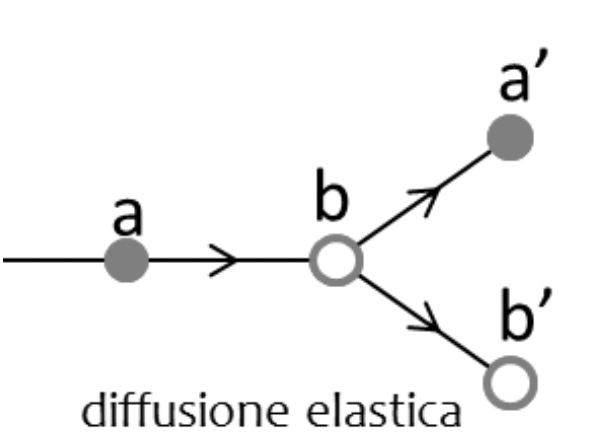
\includegraphics{figs/diffusione-elastica}
	%    \caption{This is a margin figure.}
	\label{fig:diffusione-elastica}
\end{marginfigure}
\begin{itemize}
	\tightlist
	\item
	\textbf{elastici} : energia della particella incidente = energia particella emergente
	\item
	\textbf{anelastici}: energia della particella incidente \(\neq\) energia particella emergente
\end{itemize}
Dato che solitamente la particella proiettile è priva di struttura
interna, a differenza di quella bersaglio, si ha diffusione
\begin{marginfigure}
	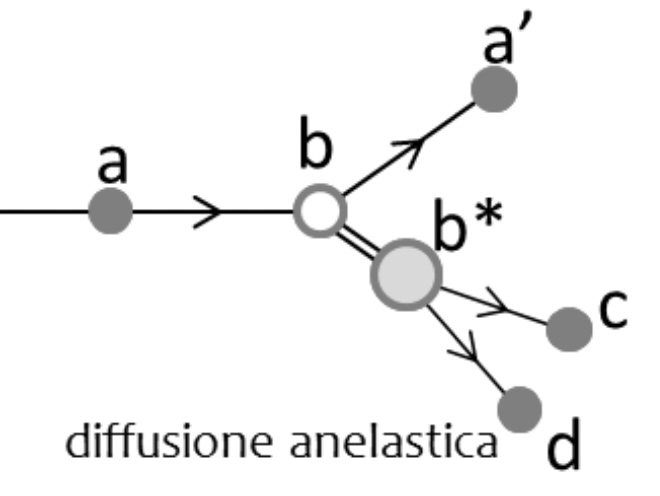
\includegraphics{figs/diffusione-anelastica}
	%    \caption{This is a margin figure.}
	\label{fig:diffusione-anelastica}
\end{marginfigure}

\begin{marginfigure}
	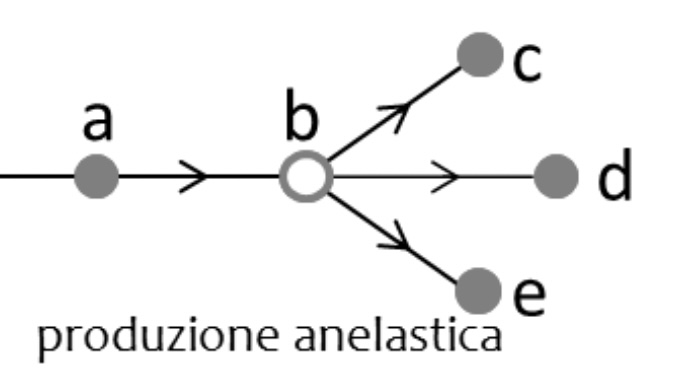
\includegraphics{figs/produzione-anelastica}
	%    \caption{This is a margin figure.}
	\label{fig:produzione-anelastica}
\end{marginfigure}

\begin{itemize}
	\item \textbf{elastica}:se il bersaglio non modifica la sua struttura e non assorbe
	energia$ \left( \Delta E^{Tot}_{cin} = 0 \right)$;
	\item \textbf{inelastica}: se il bersaglio modifica la sua struttura e assorbe energia.
\end{itemize}
A seguito della diffusione la particella bersaglio può decadere in nuove particelle in un processo noto come
\textbf{produzione inelastica} (chiaramente l'elasticità non si può avere, sulla base della terminologia introdotta)
caratterizzata da $\left( \Delta E^{Tot}_{cin} \neq 0 \right)$.
Si parla di \emph{diffusione profondamente inelastica} quando l'energia
della particella proiettile è tale che la De Broglie wavelength ad essa
associata risulta molto minore della dimensione della particella
bersaglio $ \rightarrow$ si può definirne la struttura interna (che
varia durante il processo).

Vogliamo ora domandarci quale \textbf{grandezza fisica microscopica del
bersaglio} sia possibile misurare con un arrangiamento sperimentale alla
Rutherford.
Per cominciare, occorre tenere presente che nella pratica
sperimentale si cerca di ottenere \textbf{un fascio di particelle
proiettile con densità e velocità uniformi e costanti} da inviare su di
un \textbf{bersaglio materiale chimicamente omogeneo}.
In generale, in
questa situazione, \textbf{si ottengono informazioni sui componenti
microscopici del bersaglio confrontando il fascio di particelle uscente
con quello entrante}.
In particolare maggiore è il numero di grandezze
fisiche del fascio emergente che vengono misurate (distribuzione
spaziale, energia, quantità di moto, tipologia, etc\ldots) più
dettagliata risulterà l'informazione sui componenti microscopici del
bersaglio.

Le assunzioni che faremo sono le seguenti:
\begin{enumerate}
	\tightlist
	\item
	il fascio di sezione trasversale \(\Sigma\) sia costituito da
	corpuscoli massivi puntiformi in moto con la stessa velocità \(v\) e
	densità spaziale \(n_f\) uniforme e costante;
	\item il bersaglio sia costituito da sferette massive di raggio dato,
	distribuite con densità \(n_b\) uniforme all'interno di un sottile
	strato materiale di spessore \(\Delta x\) e area maggiore di
	\(\Sigma\) (in modo da utilizzare tutte le particelle del fascio);
	\item
	l'interazione tra particella proiettile e particella bersaglio sia
	assimilabile ad un urto meccanico;
	\item
	a seguito di tale interazione la particella proiettile venga deviata e
	dunque rilevata in una direzione diversa da quella del fascio.
\end{enumerate}
Date queste condizioni, la probabilità che una singola particella
proiettile $ p^{(i)}_f$ interagisca con una singola particella del bersaglio $ p^{(j)}_b$ vale
\[
	\frac{\sigma}{\Sigma}
\]
dove \(\sigma\) è la sezione trasversale della particella bersaglio e \(\Sigma\) la sezione trasversale del fascio.
In pratica, detto \(\Delta N_f\) il numero di particelle del fascio che nel tempo \(\Delta t\) hanno avuto la
possibilità di interagire con le \(\Delta N_b\) particelle del bersaglio, si ha un \emph{numero di particelle deflesse
dalla direzione del fascio} a seguito dell'urto pari a
\[
	\Delta N_{def} = \sum_{j}^{\Delta N_b} \sum_{i}^{\Delta N_f} \frac{\sigma}{\Sigma}=
	\Delta N_f \Delta N_b \frac{\sigma}{\Sigma}
\]

Ora si noti che le \(\Delta N_f\) particelle del fascio sono contenute
all'interno di un parallelepipedo di area \(\Sigma\) ed altezza
\(v \Delta t\) mentre le \(\Delta N_b\) particelle del bersaglio sono
contenute all'interno di un parallelepipedo di area \(\Sigma\) ed
altezza \(\Delta x\).
Ricordando allora che le densità volumetriche di particelle del fascio e del bersaglio valgono
rispettivamente \(n_f\) e \(n_b\), si ottengono le seguenti espressioni:
\[
	\Delta N_f = \underbrace{\Sigma v \Delta t}_{ \text{Volume}}n_f
	\qquad
	\Delta N_b = \underbrace{\Sigma  \Delta x}_{ \text{Volume}}n_b
\]
che sostituite forniscono il numero di particelle deflesse nel tempo
\(\Delta t\):
\[
	\Delta N_{def} = \Delta N_f \Delta N_b \frac{\sigma}{\Sigma} =
	(\Sigma v \Delta t \ n_f)(\Sigma \Delta x \ n_b)\frac{\sigma}{\Sigma}
\]
e quindi un rate di deflessione
\[
	\frac{\Delta N_{def}}{\Delta t} = (v n_f)( \Sigma \Delta x n_b) \sigma
\] Invertendo la relazione, otteniamo infine l'espressione della
\textbf{sezione trasversale della particella bersaglio} o
\textbf{sezione d'urto}
\begin{equation}
	\boxed{\  \sigma = \frac{1}{(n_fv)(n_b \Sigma \Delta x)}\frac{dN_{def}}{dt} }
	\label{eq:cross-section-def}
\end{equation}
L'interesse di questa espressione risiede nel fatto che mette in
relazione una grandezza fisica microscopica, quale la sezione
trasversale \(\sigma\) della particella bersaglio, con grandezze fisiche
macroscopiche misurabili quali sono i parametri geometrici
\(n_f,n_b,\Sigma,\Delta x\) e \(\frac{\Delta N_{def}}{\Delta t}\).

La grandezza \(\sigma\) è detta \textbf{sezione d'urto totale} o \emph{sezione
totale d'interazione} ed è ciò che può essere misurato in un tipico
arrangiamento alla Rutherford (questa affermazione va presa cum grano
salis poiché disponendo di un adeguato apparato si possono misurare le
sezioni d'urto in funzione di specifiche variabili d'interesse), ha le
\textbf{dimensioni di un'area} (in questo caso coincidente con l'area
trasversale della particella bersaglio) e dunque si misura in
\(m^2\) (più propriamente in suoi sottomultipli), ed è la grandezza
fisica che \textbf{caratterizza l'interazione tra la generica particella
del fascio e la generica particella del bersaglio}.
Ci attendiamo infine che tale espressione abbia una \textbf{validità generale} e che possa
essere applicata non solo nel caso specifico dell'urto meccanico da noi
esaminato (impossibile a livello microscopico!) ma anche nel caso più
realistico in cui le particelle del fascio e del bersaglio interagiscono
per mezzo di una interazione naturale.

Infatti, anche nel caso delle particelle subatomiche, nel quale la mutua
interazione non è certo schematizzabile come un urto meccanico di sfere
rigide, sarà sempre possibile introdurre la grandezza microscopica
\(\sigma\) il cui valore, però, non sarà determinato dalla sezione
trasversale della particella ma dalle proprietà della interazione e tra
particella proiettile e particella bersaglio.

Dunque, in fisica nucleare e delle particelle elementari gli esperimenti
su fasci misurano essenzialmente le sezioni d'urto della interazione
elementare fascio-bersaglio.
Quando si dispone di una teoria
quantitativa di tale interazione la grandezza $\sigma$ può essere
calcolata anche teoricamente ed allora, attraverso il confronto con il
valore determinato sperimentalmente, risulta possibile saggiare la bontà
della teoria stessa.
Nella fisica nucleare e delle particelle elementari
il confronto tra teoria ed esperimento avviene quasi sempre attraverso
le sezioni d'urto.

Se l'apparato sperimentale è costruito in modo opportuno risulta
possibile andare oltre il semplice conteggio del numero di particelle
deflesse e fornire informazioni sempre più stringenti.
Ad esempio, con un apparato sperimentale disposto attorno al bersaglio e
\emph{opportunamente segmentato}, in un processo di scattering risulta
possibile misurare la distribuzione angolare delle particelle del fascio
deflesse dal bersaglio acquisendo un'ulteriore informazione sperimentale
sulle proprietà della interazione in gioco.
\begin{marginfigure}
	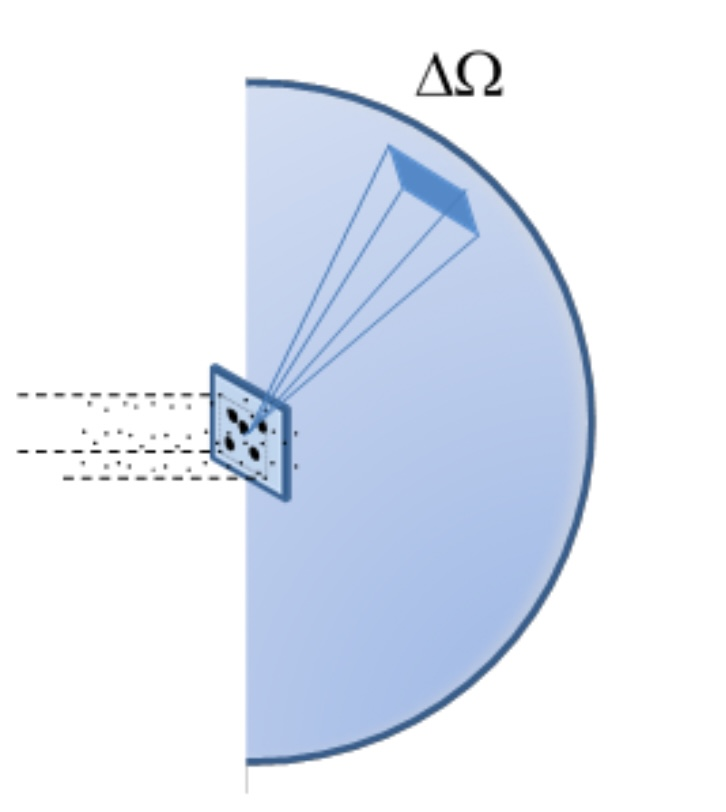
\includegraphics{figs/solid-angle-cross-section}
	%    \caption{This is a margin figure.}
	\label{fig:solid-angle-cross-section}
\end{marginfigure}
In questo modo si potrà misurare la sezione d'urto d'interazione con la condizione ulteriore che
la particella proiettile emerga all'interno di un certo angolo solido
elementare \(d \Omega\).
Avremo allora la seguente d'urto elementare
(poiché infinitesimo risulta l'elemento di angolo solido)

\marginnote{Sezione d'urto differenziale \\
	rispetto all'angolo solido}
\[
	d \sigma = \frac{1}{(n_fv)(n_b \Sigma \Delta x)}d \left( \frac{dN_{def}}{dt} \ \text{in} \ d\Omega\right)
\]
in altri termini:
\[
	d \sigma = \frac{1}{(n_fv)(n_b \Sigma \Delta x)} \frac{d\dot{N}_{def \ in \ \Delta \Omega}}{d \Omega} d \Omega
\]
dalla quale otteniamo l'espressione della \textbf{sezione d'urto
differenziale rispetto all'angolo solido} che è la grandezza misurata
dal nostro ipotetico esperimento.
Va da sè che l'integrale di tale
sezione d'urto differenziale rispetto all'angolo solido debba restituire
la sezione d'urto totale
\begin{equation}
	\boxed{ \sigma = \iint_{\Omega}\frac{d \sigma}{d \Omega} \, d \Omega }
	\label{eq:cross-section-solid-angle}
\end{equation}
relazione che può essere assunta come definizione della sezione d'urto
differenziale rispetto all'angolo solido.
Se il rivelatore permette di misurare anche l'energia della particella proiettile sarà possibile
misurare il numero di particelle del fascio che nella unità di tempo
emergono nell'angolo solido elementare \(d \Omega\) all'interno
dell'intervallo elementare \(dE\).
Si ha infatti:
\begin{gather*}
	\frac{d \sigma}{d \Omega} = \frac{1}{(n_fv)(n_b \Sigma \Delta x)}\frac{d}{d \Omega} \left( \frac{dN_{def}}{dt} \ \text{in} \ d\Omega\right)\\
	\frac{d^2 \sigma}{dE d \Omega} = \frac{1}{(n_fv)(n_b \Sigma \Delta x)}\frac{d}{dE}\frac{d}{d \Omega} \left( \frac{dN_{def}}{dt} \ \text{in} \ d\Omega \ \text{e} \ dE\right)
\end{gather*}
Il nostro ipotetico esperimento misurerà allora la seguente
\textbf{sezione d'urto doppiamente differenziale in funzione dell'angolo
solido e della energia} definita dalla relazione
\[
	\sigma = \iint_{\Omega}\int_{E} \frac{d^2 \sigma}{dE d \Omega} \, dE \ d \Omega
\]
Gli esempi citati, pur riferendosi a casi particolari chiariscono il fatto, di validità generale, che \emph{il tipo di sezione d'urto misurata dipende essenzialmente dalle caratteristiche tecniche del rivelatore}.

Nel caso più semplice si misurerà una sezione d'urto totale di interazione ma, disponendo di rivelatori via via più sofisticati, risulterà possibile misurare sezioni d'urto differenziali di interazione in funzione di un insieme di variabili cinematiche sempre più ampio.

%%%%%%%%%%%%%%%%%%%%%%%%%%%%%%%%%%%%%%%%%%%%%%%%%%%%%%%%%%%%%%%%%%%%%%%%%%%%%%%%%%%%%%%%%%%%%%%%%%%%%%%%%%%%%%%%%%%%%%%%
\section{Calcoli di sezioni d'urto}\label{sec:calcoli-di-sezioni-d'urto}
%%%%%%%%%%%%%%%%%%%%%%%%%%%%%%%%%%%%%%%%%%%%%%%%%%%%%%%%%%%%%%%%%%%%%%%%%%%%%%%%%%%%%%%%%%%%%%%%%%%%%%%%%%%%%%%%%%%%%%%%
Vediamo due esempi di calcolo di sezioni d'urto :
\begin{description}
	\item[i.] Sezione d'urto differenziale rispetto all'angolo solido di un fascio di proiettili di sezione trascurabile su sfere di raggio $R$ nella ipotesi che abbiano luogo urti classici elastici;
	\item[ii.] Sezione d'urto differenziale di Rutherford.
\end{description}

\smallcaps{ Caso \emph{i}}.
Senza entrare nel dettaglio della meccanica dell'urto - assumendo un sistema di coordinate sferiche con asse z lungo l'asse centrale della sfera - sappiamo che sussiste una piena simmetria rispetto all'angolo e l'\textbf{angolo di emergenza} del proiettile è interamente determinato dal \textbf{parametro d'urto} $b$ attarverso una relazione del tipo
\begin{equation}
	b = b(\theta)
	\label{eq:cross-sec-calc1}
\end{equation} che codifica i dettagli dell'urto stesso.

\begin{figure}
	\centering
	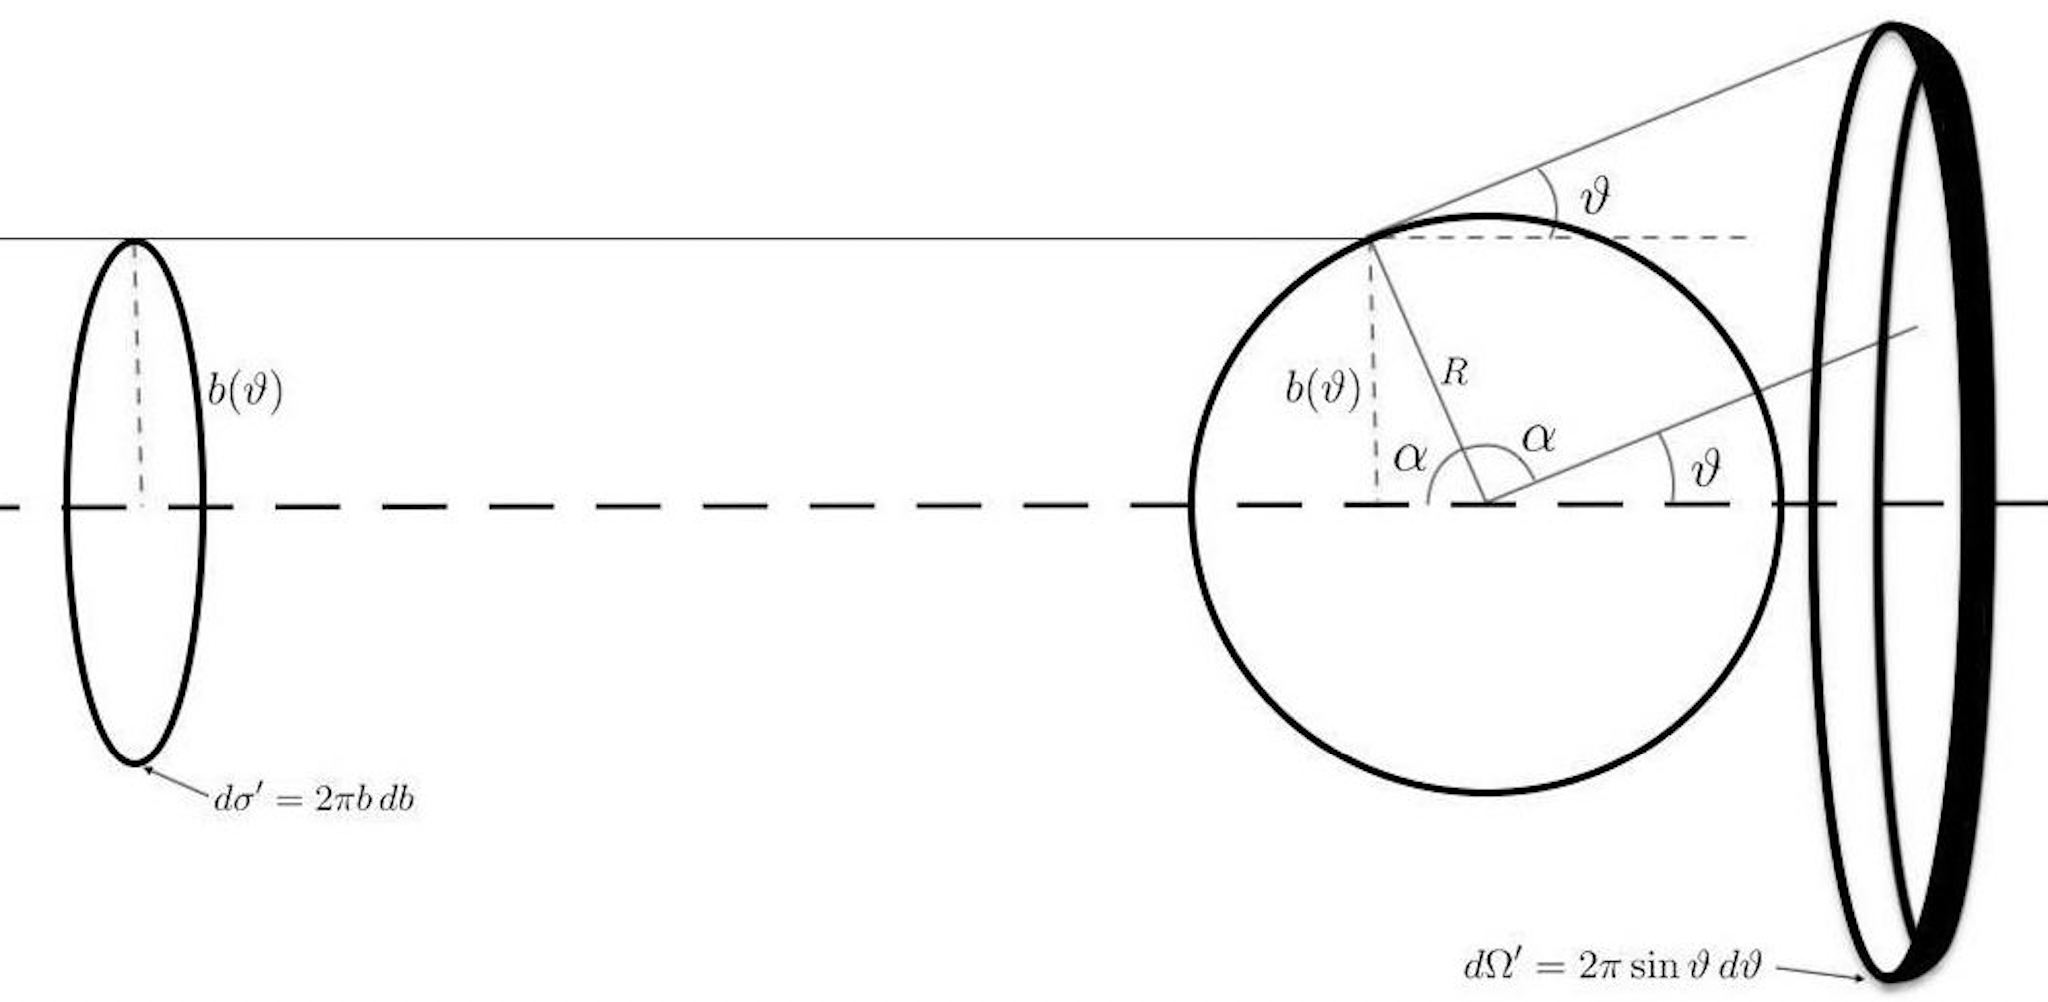
\includegraphics{figs/ex-cross-section}
	\caption{Calcolo della sezione d'urto differenziale rispetto all'angolo solido di un fascio su sfere di raggio noto
	nell'ipotesi di urti classici elastici.}
	\label{fig:ex-cross-section}
\end{figure}
Facendo riferimento allo schema in figura~\ref{fig:ex-cross-section} si ha
\begin{gather*}
    d \sigma' = \int d \sigma = 2 \pi b(\theta) \, db\\
    d \Omega' = \int d \Omega = \int_{0}^{2 \pi} d \varphi \sin(\theta) d \theta = 2 \pi \sin(\theta) \, d \theta
\end{gather*}
e inoltre dalla definizione di angolo solido:
\[
 d \Omega = \frac{dS}{{r}^{2}}= \sin (\theta) \, d \theta d \varphi
\]
Riusciamo quindi a scrivere la nostra sezione d'urto doppiamente differenziale, sulla base di
(\ref{eq:cross-section-solid-angle}):
\[
	d \sigma = \frac{d \sigma}{d \Omega}d \Omega
	= \frac{2 \pi b \, db}{2 \pi \sin(\theta) d \theta} \sin(\theta) d \theta d \varphi
	=  b d \varphi db
\]
Ciò significa che tutti i proiettili passanti per l'area elementare $bd \varphi db$ saranno deflessi dello stesso angolo
solido elementare $d \Omega$.
Da qui segue
\[
	\frac{d \sigma }{d \Omega} \sin (\theta) d \varphi d \theta   =  b d \varphi \left |\frac{db}{d \theta}\right | d \theta
\]
e dunque, infine, la sezione d'urto differenziale rispetto all'angolo solido
\begin{equation}
	\frac{d \sigma}{d \Omega} = \frac{b}{sin (\theta)}\left |\frac{db}{d \theta}\right |
	\label{eq:cross-sec-calc2}
\end{equation} valida classicamente non solo nel caso della sfera rigida ma in generale.

Per calcolare la sezione d'urto differenziale rispetto all'angolo solido nel caso della sfera rigida di raggio R dobbiamo
ora precisare la forma della (\ref{eq:cross-sec-calc1}).
Si trova facilmente
\[
	\frac{b}{R} = \sin{\alpha}  \qquad \theta = \pi - 2 \alpha
\]
da cui
\[
	b = R \cos{\frac{\theta}{2}}
\]
Sostituendo nella (\ref{eq:cross-sec-calc2}) otteniamo
\[
	\frac{d \sigma}{d \Omega} = \frac{R \cos{\frac{\theta}{2}}}{\sin \theta} \left | \frac{d}{d \theta}R \cos{\frac{\theta}{2}} \right | = \frac{R \cos{\frac{\theta}{2}}}{\sin \theta}\frac{R}{2} \sin \frac{\theta}{2}
\]
da cui, infine, la sezione d'urto differenziale della sfera rigida di raggio $R$
\begin{equation}
	\frac{d \sigma}{d \Omega} = \frac{R^2}{4}
	\label{eq:cross-section-rigid-sphere}
\end{equation}

E' immediato verificare che da questa espressione si ottiene una sezione d'urto totale $\sigma = \pi R^2$.

\marginnote{Sezione d'urto differenziale di una sfera rigida}

La formula (\ref{eq:cross-section-rigid-sphere}) può essere utilizzata \emph{anche nel caso in cui l'interazione} tra le
particelle del fascio e quelle del bersaglio \emph{non consista in un urto meccanico} ma in una interazione mediata da una
forza naturale.

\smallcaps{Caso} \emph{ii}.
Trattiamo allora il caso della \textbf{diffusione di Rutherford} di proiettili di carica elettrica positiva $ze$ su 
bersagli di carica elettrica positiva $Ze$ governata dalla forza
\[
	\bm{F} = \frac{zZe^2}{4 \pi \epsilon_0}\frac{1}{r^2}\hat{\bm{r}}
\]
con potenziale associato 
\[
    V = \frac{zZ {e}^{2}}{4 \pi \epsilon_0 } \frac{1}{r}
\]
Dalla seconda equazione cardinale si ha
\[
      \bm{r} \wedge \bm{F} = \dot{\bm{L}}
\]
per cui, come noto tale forza \textbf{conserva il momento angolare} del proiettile:
\[
	  \bm{r} \wedge \bm{F} = r \hat{\bm{r}} \wedge \frac{zZe^2}{4 \pi \epsilon_0}\frac{1}{r^2}\hat{\bm{r}} = 0 \rightarrow
	  \dot{\bm{L}} = \bm{0} \rightarrow \bm{L} = \bm{cost}
\]
Ciò implica
\[
	\bm{L}_{t \to - \infty} = \bm{L}_t \qquad
	\left( \bm{r} \wedge m \bm{v} \right)_{- \infty} = \left( \bm{r} \wedge m \bm{v} \right)_{t}
\]
Tenendo conto delle seguenti condizioni al contorno
\[
    x_{ - \infty} \leq 0  , \ \dot{x}_{- \infty} = v_0 \qquad y_{- \infty} = b , \  \dot{y}_{- \infty} = 0
\]
la precedente si  riscrive come(il secondo termine è stato scritto in coordinate polari piane)
\[
	(-x \hat{\bm{i}} + y \hat{\bm{j}}) \wedge (m \dot{x} \hat{\bm{i}} + m \dot{y} \hat{\bm{j}})_{- \infty} =
	r \hat{\bm{r}} \wedge m(\dot{r}\hat{\bm{r}} + r \dot{\varphi}\hat{\varphi})
\]
da cui si ottiene
\[
   - \dot{x}y = {r}^{2} \dot{\varphi}
\]
\begin{equation}
	\dot{\varphi} = - \frac{v_0 \ b}{r^2}
	\label{eq:ex-cross-section2-1}
\end{equation}
Sfruttiamo ora la conservazione dell'energia:
\begin{gather*}
    T_{- \infty} + V_{- \infty} = T_{\infty} + V_{\infty}\\
    V_{\pm \infty} = - \frac{zZ {e}^{2}}{4 \pi \epsilon_0 } \frac{1}{r_{\pm \infty}} = 0 \rightarrow
	T_{- \infty}  = T_{\infty}
\end{gather*}
ed otteniamo
\begin{equation}
	v_0 = v_{\infty}
	\label{eq:ex-cross-section2-2}
\end{equation}
Fatte queste premesse conviene risolvere la sola \textbf{equazione del moto trasversale}:
\begin{gather*}
	F_y = \frac{d}{dt}m v_y \quad \ \frac{zZe^2}{4 \pi \epsilon_0}\frac{1}{r^2}\sin \varphi = \frac{d}{dt}mv_y\\
	mv_{y,t= + \infty} - mv_{y,t = - \infty} = \int_{- \infty}^{+\infty} \frac{zZe^2}{4 \pi \epsilon_0}\frac{1}{r^2}\sin \varphi\,dt
\end{gather*}
Dalle condizioni al contorno
\[
	v_{y,t= + \infty} = v_{t= + \infty}\sin \theta \qquad v_{y,t = - \infty} = 0 \quad \varphi_{t = +\infty} = \theta \quad \varphi_{t = - \infty} = \pi
\]
e usando (\ref{eq:ex-cross-section2-1}) si ottiene
\[
	mv \sin \theta = - \int_{- \infty}^{+ \infty} \frac{zZe^2}{4 \pi \epsilon_0}\frac{1}{r^2}\sin \varphi
	\frac{r^2}{v_0b}\,d \varphi = \frac{zZe^2}{4 \pi \epsilon_0 v_0 b}(\cos \theta + 1)
\]
da cui
\begin{equation}
	b = \frac{zZe^2}{4 \pi \epsilon_0 m v^2_0} \cot \frac{\theta}{2}
	\label{eq:ex-cross-section2-3}
\end{equation}
Ora possiamo derivare questa espressione
\[
	\left | \frac{db}{d \theta}\right | = \frac{1}{2}\frac{zZe^2}{4 \pi \epsilon_0 m v^2_0}\frac{1}{\sin^2{\theta/2}}
\]
e sostituirla nella (\ref{eq:cross-sec-calc2}) assieme alla (\ref{eq:ex-cross-section2-2}) ottenendo
\[
	\frac{d \sigma }{d \Omega} = \left( \frac{zZe^2}{4 \pi \epsilon_0m v^2_0}\right) \cot{\frac{\theta}{2}}\frac{1}{2 \sin{\theta / 2 \cos (\theta /2)}}\frac{1}{2}\left( \frac{zZe^2}{4 \pi \epsilon_0m v^2_0}\right)\frac{1}{\sin^2{\theta/2}}
\]
da cui la \textbf{sezione d'urto differenziale di Rutherford}

\begin{equation}
	\frac{d \sigma }{d \Omega} = \frac{1}{4} \left( \frac{zZe^2}{4 \pi \epsilon_0m v^2_0}\right) ^2\frac{1}{\sin^4{\theta / 2}}
\end{equation}
un risultato valido anche in meccanica quantistica.

[Esercizio in dispensa pag 38.]

%%%%%%%%%%%%%%%%%%%%%%%%%%%%%%%%%%%%%%%%%%%%%%%%%%%%%%%%%%%%%%%%%%%%%%%%%%%%%%%%%%%%%%%%%%%%%%%%%%%%%%%%%%%%%%%%%%%%%%%%
\section{Le proprietà ondulatorie delle particelle microscopiche}\label{sec:proprieta-ondulatorie-delle-particelle-microscopiche}
%%%%%%%%%%%%%%%%%%%%%%%%%%%%%%%%%%%%%%%%%%%%%%%%%%%%%%%%%%%%%%%%%%%%%%%%%%%%%%%%%%%%%%%%%%%%%%%%%%%%%%%%%%%%%%%%%%%%%%%%

Nel 1913, quando Geiger, Mursden e Rutherford compirono il loro
esperimento, interpretarono le collisioni tra particelle del fascio e
atomi del materiale in termini di urti governati dalle leggi della
meccanica classica.
Non potevano fare altrimenti, tuttavia di li poco
Bohr - sulla base dei lavori di Plank ed Einstein - e poi nella decade
successiva De Broglie, Heisenberg, Schrödinger e Born modificheranno
radicalmente il quadro interpretativo introducendo l'idea che \textbf{le
particelle microscopiche, oltre a possedere proprietà corpuscolari,
	dovevano possedere anche proprietà ondulatorie,} per cui ad esse si
doveva associare una lunghezza d'onda e frequenza (De Broglie) ed una
funzione d'onda (Born), soluzione quest'ultima di una determinata
equazione d'onda (Schrödinger), giungendo così alla formulazione della

D'altra parte, a partire dai lavori di Planck sul corpo nero (1900) e di
Einstein sull'effetto fotoelettrico (1905), venne contemporaneamente
affermandosi l'idea che i campi classici maxwelliani - dotati certamente
di proprietà ondulatorie poiché capaci dei fenomeni della interferenza e
diffrazione -- dovevano essere costituiti da enti microscopici (poi
chiamati quanti del campo) dotati anche di proprietà corpuscolari.
Si affermò così il concetto di \textbf{quanto del campo come ente
microscopico intrinsecamente `ibrido' poiché dotato di proprietà sia
ondulatorie che corpuscolari}.
Dato questo stato di cose, si pose naturalmente la domanda se le particelle microscopiche ed i quanti del campo -
entrambi dotati di proprietà sia corpuscolari che ondulatorie - dovessero essere pensati come enti distinti oppure no.

La risposta -- fondamento del moderno punto di vista - fu data dalle
teorie di campo quantizzato (formulate alla fine degli anni '20 da
Dirac, Heisenberg, e Jordan) le quali assumono che \textbf{le particelle
microscopiche osservate negli apparati sperimentali devono essere
identificate con i quanti di specifici campi}, superando in tal modo la
ripartizione degli enti fisici in particelle materiali e campi affermata
dalla fisica classica.
Da ciò consegue che \textbf{il linguaggio
naturale della fisica delle particelle debba essere quello della teoria
dei campi quantizzati} tuttavia, quando le energie in gioco non sono
così elevate da rendere necessaria una descrizione relativistica e
soprattutto da rendere possibili processi di creazione e distruzione di
particelle\textbf{, la descrizione offerta dalla meccanica quantistica
ordinaria risulta appropriata}.

Per questo, alle basse e medie energie possiamo certamente assumere che
la fisica nucleare possa essere ben descritta nell'ambito della
meccanica quantistica mentre questo non è certamente più vero nella
fisica nucleare alle alte energie dove possono aversi collisioni tra
nucleoni ad energie di centinaia o migliaia di GeV per nucleone (Alice
ha operato a 2.76 TeV per coppia di nucleoni) e risulta necessaria una
descrizione dei processi basata sulle teorie di campo quantizzato.

Volendo richiamare in modo diretto ed euristico alcuni concetti di
meccanica quantistica, si può cominciare scrivendo \textbf{le grandezze
cinematiche fondamentali di una generica onda piana sinusoidale,} ovvero
la \textbf{pulsazione} ed il \textbf{vettore d'onda} collegate tra loro
nella \textbf{relazione di dispersione} che caratterizza le proprietà
fisiche del mezzo in cui l'onda stessa si propaga
\[
	\omega = \frac{2 \pi}{T} \quad \bm{k} = \frac{2 \pi}{\lambda}\hat{k} \quad \omega = \omega(\bm{k})
\]
Scriviamo anche \textbf{le grandezze cinematiche fondamentali di un
generico corpuscolo libero} che corrispondono alle espressioni
relativistiche della \textbf{energia} e \textbf{quantità di moto}
collegate dalla \textbf{relazione energia-impulso}
\begin{equation}
	E = \frac{m c^2}{\sqrt{1 - \frac{v^2}{c^2}}} \qquad \bm{p} = \frac{m \bm{v}}{\sqrt{1 - \frac{v^2}{c^2}}} \qquad
	E^2 = p^2 c^2 + m^2 c^4
	\label{eq:energy-momentum-rel}
\end{equation}

Sulla base di considerazioni di natura assai generale, Einstein e De
Broglie ipotizzarono che \textbf{le grandezze ondulatorie e corpuscolari
fossero legate dalle seguenti relazioni} (valide sia nella meccanica
quantistica che nella teoria dei campi quantizzati)
\[
	E = \hp \omega \qquad \bm{p} = \hp \bm{k}
\]
per cui dedussero il seguente legame esplicito tra grandezze
ondulatorie e corpuscolari valido per le particelle microscopiche e le
non meglio precisate \textbf{`onde quantomeccaniche'} o \textbf{`onde di
De Broglie'} a loro associate
\marginnote{Equazioni di De Broglie-Einstein}
\begin{equation}
	E = \hp \omega = \frac{m c^2}{\sqrt{1 - \frac{v^2}{c^2}}} \qquad
	\bm{p} = \hp \bm{k} = \frac{m \bm{v}}{\sqrt{1 - \frac{v^2}{c^2}}} \qquad
	\omega^2 = k^{2} c^2+ \frac{m^{2} c^4}{\hp^2}
	\label{eq:de-broglie-einstein-rel}
\end{equation}

La relazione dispersione (relazione energia-impulso) indica chiaramente
che le componenti di Fourier delle `onde quantomeccaniche' si propagano
come se il vuoto fosse un \textbf{mezzo dispersivo}.
Se ad una particella materiale si devono associare grandezze ondulatorie
ad essa si dovrà pure associare una fase ed una certa funzione della
fase detta \textbf{funzione d'onda} il cui significato fisico dovrà
essere precisato.
Una data componente di Fourier di tale onda in forma
piana dovrà comunque avere la seguente semplice espressione\sidenote{L'utilizzo
della notazione complessa non è casuale. Infatti alle due espressioni
	\[
		\psi_1(\bm{r},t) = \psi_0 e^{i(\bm{k \cdot r}-\omega t)}
	\] \[
		\psi_2(\bm{r},t) = \psi_0 \sin (\bm{k \cdot r}-\omega t)
	\] sono associate probabilità differenti \[
		| \psi_1^2| = \psi_0^2
	\] \[
		| \psi_2^2| = \psi_0^2 \sin^2(\bm{k \cdot r}-\omega t)
	\] di cui \emph{solo la prima è in accordo con le verifiche sperimentali}.}
\begin{equation}
	\psi(\bm{r},t) = \psi_0 e^{i(\bm{k \cdot r}-\omega t)} = \psi_{0} e^{\frac{i}{\hp}(\bm{p \cdot r}-E t)}
	\label{eq:wave-function-expr}
\end{equation}
Come in un qualunque fenomeno ondulatorio, data la
funzione d'onda si pone il problema di stabilire \textbf{l'equazione
d'onda} ovvero l'equazione che ne governa la dinamica.

Trovare l'espressione formale della equazione d'onda in modo diretto per
una data componente di Fourier non è difficile poiché sappiamo che una
volta sostituita la funzione d'onda (\ref{eq:wave-function-expr}) essa non deve fare altro
che restituire la relazione energia-impulso (\ref{eq:energy-momentum-rel}) o la relazione di
dispersione (\ref{eq:de-broglie-einstein-rel}).
A questo scopo vale la pena introdurre le seguenti \textbf{operazioni di differenziazione}
\begin{gather}
	- i \hp \nabla \psi (\bm{r},t) = - i \hp \nabla \psi_{0} e ^{\frac{i}{\hp}(\bm{p \cdot r}-E t)} =
	- i \hp \psi_{0} e^{\frac{i}{\hp}(\bm{p \cdot r}-E t)} \frac{i}{\hp} \bm{p} = \bm{p}\psi(\bm{r},t) \nonumber\\
	i \hp \frac{\partial}{\partial t} \psi (\bm{r},t) =
	i \hp \frac{\partial}{\partial t} \psi_{0} e^{\frac{i}{\hp}(\bm{p \cdot r}-E t)} =
	i \hp \psi_{0} e^{\frac{i}{\hp}(\bm{p \cdot r}-E t)} \left( - \frac{i}{\hp} E\right) = E\psi(\bm{r},t)
	\label{eq:differential-operators-qm}
\end{gather}
Le precedenti relazioni mostrano che gli operatori differenziali, agendo
sulla generica componente di Fourier, ne determinano la
rimoltiplicazione per i valori della quantità di moto ed energia, un
fatto che suggerisce di definirli come \textbf{operatori della quantità
di moto} ed \textbf{energia}:
\begin{itemize}
	\item Operatore della \textbf{quantità di moto}
	\[
	   \hat{P} = - i \hp \nabla    \qquad
	\]
	\item Operatore \textbf{dell'energia}
	\[
		\hat{E} = i \hp \frac{\partial}{\partial t}
	\]
\end{itemize}
Nel linguaggio degli operatori, le precenti espressioni possono allora
essere rilette affermando che in una data componente di Fourier
dell'onda quantomeccanica \textbf{i valori della quantità di moto e
della energia sono autovalori degli operatori} \(\hat{P}\) ed
\(\hat{E}\) mentre la funzione d'onda è un loro autostato
\[
	\hat{P}\psi(\bm{r},t) = \bm{p}\psi(\bm{r},t) \qquad
	\hat{E}\psi(\bm{r},t) = E\psi(\bm{r},t)
\]
Introdotti gli operatori energia e quantità di moto, possiamo
partire dalla relazione relativistica energia-impulso della particella
libera ed ottenere la sua equazione d'onda.
I passaggi sono i seguenti
\begin{gather*}
	E^2 = p^2c^2 + m^2c^4\\
	E^2\psi(\bm{r},t) = p^2c^2\psi(\bm{r},t)+m^2c^4\psi(\bm{r},t)\\
	\left( i \hp \frac{\partial}{\partial t}\right)\left( i \hp \frac{\partial}{\partial t}\right)\psi(\bm{r},t) = c^2 (-i \hp \nabla)(-i \hp \nabla)\psi(\bm{r},t)+m^2c^4 \psi(\bm{r},t)
\end{gather*}
Si noti che \textbf{tale equazione è lineare per cui deve valere non
solo per la data componente di Fourier ma -- in modo del tutto generale
- per una qualunque sovrapposizione di componenti di Fourier e dunque
per una qualsiasi onda}.

Giungiamo così ad individuare \textbf{l'equazione d'onda} cercata detta
\textbf{equazione di Klein-Gordon} valida per le '\textbf{onde
quantomeccaniche' libere scalari} (senza spin, essendo \(\psi\) scalare)
\marginnote{Equazione di Klein-Gordon}

\begin{equation}
	\nabla^2 \psi(\bm{r},t) - \frac{1}{c^2}\frac{\partial^2}{\partial t^2}\psi(\bm{r},t) =
	\frac{m^2c^2}{\hp^2}\psi(\bm{r},t)
	\label{eq:klein-gordon}
\end{equation}
Tale equazione fu trovata per la prima volta da Schrödinger il quale
però non riuscì a fornire una interpretazione fisica consistente della
funzione d'onda.
Si trattava di un problema cruciale che poteva essere
superato solo interpretando la funzione d'onda nel senso della teoria
dei campi quantizzati.
Non essendoci allora i presupposti per
un passaggio di tal genere, Schrödinger rinunciò alla equazione d'onda
relativistica e ripiegò sulla \textbf{equazione d'onda classica} la cui
interpretazione sembrava meno problematica.
Tale equazione la si può
ottenere seguendo esattamente lo stesso tipo di procedimento partendo
però dalla espressione \textbf{energia-impulso classica delle particelle libere}
\[
	E = \frac{p^2}{2m}
\]
Compreso questo fatto, possiamo puntare direttamente a costruire
\textbf{l'equazione d'onda non relativistica per le `onde
quantomeccaniche' in presenza di forze} aggiungendo il loro potenziale
alla espressione precedente
\[
	E = \frac{p^2}{2m} + V(\bm{r})
\]
Nel caso di una generica componente di Fourier otteniamo allora
\begin{gather*}
	E = \frac{p^2}{2m} + V(\bm{r}) \rightarrow E \psi(\bm{r},t) = \frac{p^2}{2m}\psi(\bm{r},t) +
	V(\bm{r},t)\psi(\bm{r},t)\\
	\left( i \hp \frac{\partial}{\partial t} \right)\psi(\bm{r},t) = \frac{1}{2m}(- i \hp \nabla)(- i \hp \nabla)\psi(\bm{r},t) + V(\bm{r})\psi(\bm{r},t)\\
	i \hp \frac{\partial}{\partial t} \psi(\bm{r},t) = - \frac{\hp^2}{2m}\nabla^2\psi(\bm{r},t)+
	V(\bm{r})\psi(\bm{r},t) = \left[ - \frac{\hp^2}{2m}\nabla^2 + V(\bm{r})\right] \psi(\bm{r},t)
\end{gather*}
Data la linearità della equazione, concludiamo che l'espressione
ottenuta deve essere valida non solo per la generica componente di
Fourier ma per una qualunque funzione d'onda.
Definendo allora
l'operatore tra parentesi come \textbf{operatore hamiltoniano}
\(\hat{H}\), otteniamo la seguente \textbf{equazione d'onda di
Schrödinger} valida per le \textbf{`onde quantomeccaniche' scalari (senza spin) non relativistiche in presenza di forze}
\marginnote{Equazione d'onda di Schrödinger}
\begin{equation}
	i \hp \frac{\partial}{\partial t} \psi(\bm{r},t) = \hat{H}\psi(\bm{r},t) \qquad
	\hat{H} = - \frac{\hp^2}{2m} \nabla^2 + V(\bm{r})
	\label{eq:schroedinger}
\end{equation}
Tale equazione rese possibile una interpretazione della funzione d'onda
che - pur non essendo di validità generale - permetteva comunque di
descrivere in modo appropriato i fenomeni quantomeccanici in regime non
relativistico ovvero alle basse e medie energie dove non avvengono
processi di creazione e/o distruzione di particelle.
Tale interpretazione fu proposta da M. Born ed afferma che
\begin{quote}
	Il modulo quadrato della funzione d'onda nella posizione $ \bm{r}$ ed al
	tempo t rappresenta la densità di probabilità di trovare la particella
	materiale in quella posizione ed in quell'istante di tempo a seguito di
	una misura di posizione.
\end{quote}
Questa ipotesi va a costituire uno dei
fondamentali assiomi interpretativi della meccanica quantistica e
comporta che l'espressione
\begin{equation}
	\left | \psi(\bm{r},t)\right |^2 dV
	\label{eq:wave-probability-density}
\end{equation}
rappresenti la probabilità di misurare la particella
materiale al tempo \(t\) all'interno del volume \(dV\) centrato nella
posizione \(\bm{r}\).

I fatti appena richiamati chiariscono che \textbf{l'interazione
particella- proiettile/particella-bersaglio non deve essere pensata come
un processo d'urto meccanico ma, piuttosto, come un processo di
diffrazione/rifrazione dell'onda quantomeccanica associata alla
particella proiettile a seguito della sua interazione con
l'ostacolo-bersaglio}.
Dunque essenzialmente un processo di `\textbf{ottica delle onde quantomeccaniche}' dipendente dal tipo di
interazione in gioco.
Se il bersaglio è totalmente riflettente risulterà un processo di
diffrazione simile a quello di un tratto di muro piazzato sul percorso
di un'onda in acqua.
Se il bersaglio è totalmente assorbente risulterà
un processo di diffrazione simile a quello di un tratto di scogliera.
Se
invece il bersaglio opera come un potenziale di forza avremo un processo
di rifrazione assimilabile alle distorsioni dei fronti d'onda
determinate dalle variazioni di profondità del fondale.
Al netto di
questi dettagli è comunque evidente che \textbf{gli esperimenti
fascio-bersaglio con particelle microscopiche devono essere interpretati
in chiave ondulatoria.}

Ad esempio, se vogliamo esplorare la struttura di un nucleo atomico
dovremo essere in grado di risolvere almeno i singoli nucleoni.
Ma l'interferenza di due onde provenienti da due diversi nucleoni è
apprezzabile solo se i cammini differiscono di una quantità dell'ordine
della lunghezza d'onda.
\begin{marginfigure}
	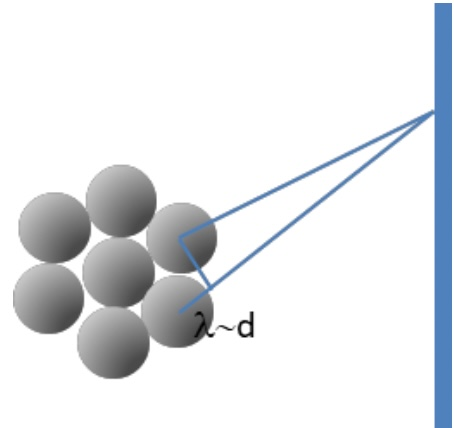
\includegraphics{figs/fascio-bersaglio-de-broglie}
	%    \caption{Sezione d'urto differenziale di una sfera rigida.}
	\label{fig:fascio-bersaglio-de-broglie}
\end{marginfigure}

D'altra parte la differenza di tali cammini è anche dell'ordine delle
dimensioni del singolo nucleone.
Ciò significa che dovremo impiegare
particelle proiettile aventi una lunghezza d'onda di De Broglie
dell'ordine delle dimensioni del singolo nucleone ovvero dell'ordine di
\(1 fm\).
In questo modo saremo sensibili agli effetti
diffrattivi-interferenziali indotti dalla struttura nucleare che potremo
osservare raccogliendo le particelle diffuse su di un rivelatore capace
di misurarne la posizione angolare.
Per quanto riguarda invece la scelta
del proiettile converrà utilizzare i neutroni dato che non risentono
della interazione elettromagnetica che andrebbe a complicare il fenomeno
(si tenga però presente che è più difficile avere a che fare con fasci e
rivelatori di neutroni!).

Ricordando che
\[
	\frac{\hp c}{200 MeV}  \simeq 1 fm
\]
si ha
\begin{gather*}
	p = \hp k = \hp \frac{2 \pi}{\lambda} = \hp \frac{2 \pi}{1} fm^{-1} = \hp 2 \pi \frac{200 MeV}{\hp c}
	\simeq 1.2 \frac{GeV}{c}\\
	\epsilon = \sqrt{p^{2} c^2+m^{2} c^4}\simeq \sqrt{(1.2)^2+(1.0)^2} \simeq 1.5 GeV
\end{gather*}
da cui si verifica che con un fascio di particelle di circa $1.2 GeV/c$ di impulso ed $1.5 GeV$ di energia si raggiunge lo scopo.
Se invece vogliamo esplorare la struttura del singolo nucleone dovremo avere un potere risolutivo almeno 100 volte superiore ovvero un impulso $100$ volte maggiore e dunque fasci di particelle di impulso dell'ordine di $100 GeV$.
%%%%%%%%%%%%%%%%%%%%%%%%%%%%%%%%%%%%%%%%%%%%%%%%%%%%%%%%%%%%%%%%%%%%%%%%%%%%%%%%%%%%%%%%%%%%%%%%%%%%%%%%%%%%%%%%%%%%%%%%
\section{Teoria della diffrazione di Kirchoff}\label{sec:teoria-della-diffrazione-di-kirchoff}
%%%%%%%%%%%%%%%%%%%%%%%%%%%%%%%%%%%%%%%%%%%%%%%%%%%%%%%%%%%%%%%%%%%%%%%%%%%%%%%%%%%%%%%%%%%%%%%%%%%%%%%%%%%%%%%%%%%%%%%%

Dato che l'interazione fascio-bersaglio consiste essenzialmente nella
diffrazione delle onde di De Broglie associate alle particelle del
fascio da parte delle particelle del bersaglio, la corretta soluzione
del problema può essere ottenuta cercando l'espressione della funzione
d'onda che:
\begin{enumerate}
	\tightlist
	\item soddisfa l'equazione di Schrödinger con potenziale nella regione in
	cui il fascio interagisce con il bersaglio;
	\item soddisfa l'equazione d'onda di Schrödinger libera nella regione
	esterna alla interazione prima e dopo il bersaglio;
	\item soddisfa la condizione al contorno di essere un'onda piana prima di
	incidere sul bersaglio.
\end{enumerate}
Seguiremo un approccio che sottolinea l'identità tra onde classiche e onde di De Broglie
utilizzando l'ottica classica.
Come noto, la diffrazione delle onde scalari classiche da parte di una
apertura puo' essere trattata in modo rigoroso per mezzo della
\textbf{teoria di Kirchhoff}, la cui trattazione formale si trova nel famoso testo di Ottica Classica
di Born~\cite{Born2019}.
In particolare, se una apertura $A$ è investita da un'onda
monocromatica, la funzione d'onda diffratta \(\psi(\bm{r})\) in un
generico punto dello spazio \(\bm{r}\) oltre lo schermo è data dalla
seguente espressione:
\begin{marginfigure}
	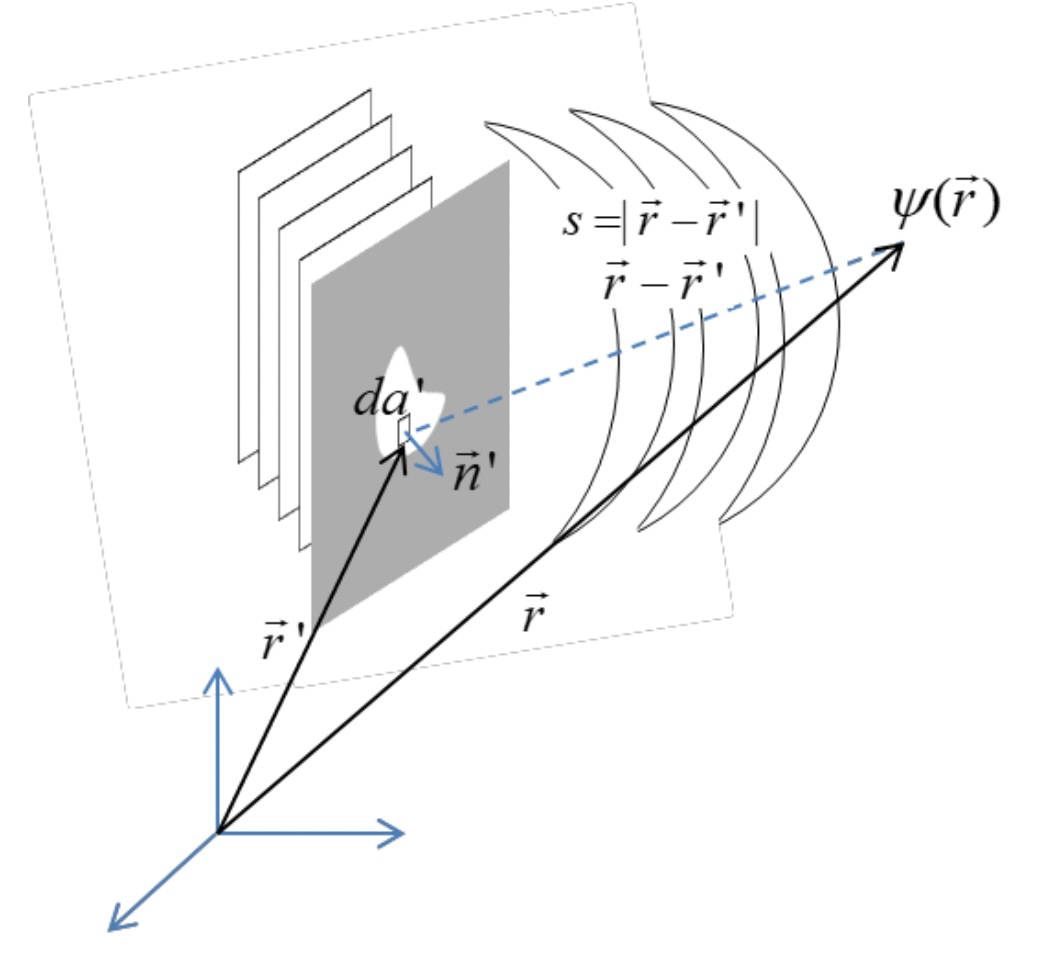
\includegraphics[width = 1.25 \textwidth, height = 1.25 \textheight]{figs/kirchhoff-diffraction-1}
	%    \caption{Sezione d'urto differenziale di una sfera rigida.}
	\label{fig:kirchhoff-1}
\end{marginfigure}

\begin{equation}
	\psi(\bm{r}) = \frac{1}{4 \pi} \mathlarger{\iint_{A}} \left[ \psi(\bm{r'}) (\bm{n}' \cdot \nabla') \frac{e^{iks}}{s} - \frac{e^{iks}}{s}(\bm{n}' \cdot \nabla') \psi(\bm{r}') \right]  \, da'
	\label{eq:kirchhoff-diffraction-formula}
\end{equation}
dove
\begin{itemize}
	\tightlist
	\item \(\bm{r}\) è il vettore posizione del punto di osservazione
	\item \(\bm{r'}\) è il vettore posizione di un punto dell'apertura
	\item \(\psi(\bm{r'})\) è la funzione d'onda calcolata nel punto \(\bm{r'}\)
	dell'apertura
	\item \(\bm{n}'\) è la normale allo schermo nel punto \(\bm{r'}\)
	dell'apertura
	\item \(\nabla'\) è il gradiente della funzione d'onda nel punto \(\bm{r'}\) dell'apertura
	\item \(\bm{k}\) è il modulo del vettore d'onda della funzione d'onda incidente
	\item \(s = | \bm{r} - \bm{r'}|\) è il modulo del vettore congiungente il punto dell'apertura con quello di osservazione
\end{itemize}
Dato che la funzione d'onda \(\psi(\bm{r})\) compare in entrambi i
membri, tale espressione richiede la conoscenza della funzione
\(\psi(\bm{r})\) stessa che si vuole determinare (questo fatto è noto
come `Paradosso di Kirchhoff').
Un circolo vizioso che viene evitato attraverso \textbf{l'approssimazione di Kirchhoff} la quale assume che la
funzione \(\psi(\bm{r})\) sia non nulla nei soli punti dell'apertura
\(A\) ed ivi coincida con la funzione d'onda monocromatica incidente(eliminando cosí il problema
dell'incurvatura dei fronti d'onda).

Consideriamo allora il caso di onda piana monocromatica diretta lungo
l'asse delle \(z\) positive incidente su di uno schermo piano normale
all'asse stesso.
Si ha
\begin{gather*}
	\psi(\bm{r}) = \psi_0 e^{i \bm{k} \cdot \bm{r}}= \psi_0 e^{ik \hat{k}(x \hat{\imath}+y \hat{\jmath}+z \hat{k})}
	= \psi_{0} e^{ikz}\\
	\bm{n}' = \hat{k}\\
	\psi(\bm{r'}) = \psi_0 e^{i \bm{k} \cdot \bm{r'}}= \psi_0 e^{ik \hat{k}(x' \hat{\imath}+y' \hat{\jmath}+z' \hat{k})}
	= \psi_{0} e^{ikz'}
\end{gather*}
e inoltre
\[
	s = |\bm{r} - \bm{r}'| = \sqrt{(x-x')^2+(y-y')^2+(z-z')^2}
\]
Sviluppiamo ora i termini presenti nell'equazione di Kirchhoff:
\begin{gather*}
	(\bm{n}' \cdot \nabla')\frac{e^{iks}}{s} = \frac{\partial}{\partial z'}\frac{e^{iks}}{s} = ik \frac{e^{iks}}{s}\frac{\partial s}{\partial z'} - \frac{e^{iks}}{s^2}\frac{\partial s}{\partial z'}  = \left( ik \frac{e^{iks}}{s}- \frac{e^{iks}}{s^2} \right)\frac{\partial s}{\partial z'}\\
	(\bm{n}' \cdot \nabla')\psi(\bm{r'}) = \frac{\partial}{\partial z'}\psi_0e^{ikz'}=ik\psi_0 e^{ikz'}
\end{gather*}
\begin{align*}
	\frac{\partial s}{\partial z'} & = \frac{\partial }{\partial z'}|\bm{r'}-\bm{r}|
	= \frac{\partial }{\partial z'}\sqrt{(x-x')^2+(y-y')^2+(z-z')^2} \\
	                               & = - \frac{1}{2s}2(z-z') = - \frac{z-z'}{s} = \cos \theta
\end{align*}
con
\[
\cos \theta = \frac{ (\bm{r'}-\bm{r})\cdot \hat{k}}{|\bm{r'}-\bm{r}|}
\]
\begin{marginfigure}
	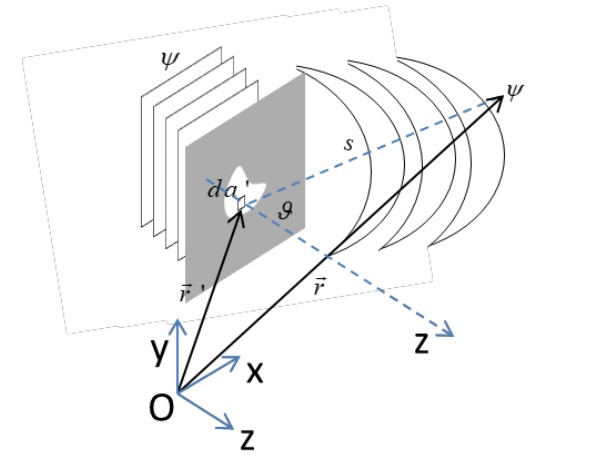
\includegraphics[width = 1.25 \textwidth, height = 1.25 \textheight]{figs/kirchhoff-diffraction-2}
	%    \caption{Sezione d'urto differenziale di una sfera rigida.}
	\label{fig:kirchhoff2}
\end{marginfigure}
Da qui si ottiene lo sviluppo del primo termine presente nell'equazione di Kirchhoff (\ref{eq:kirchhoff-diffraction-formula}):
\[
	(\bm{n}' \cdot \nabla')\frac{e^{iks}}{s} = -\left(ik\frac{e^{iks}}{s}-\frac{e^{iks}}{s^2}\right) \cos \theta
\]
Sostituendo infine le espressioni di $(\bm{n}' \cdot \nabla ') \frac{e^{iks}}{s}$ e di
$(\bm{n}' \cdot \nabla')\psi(\bm{r'})$ in (\ref{eq:kirchhoff-diffraction-formula}) otteniamo
\[
	\psi(\bm{r}) = \frac{1}{4 \pi} \mathlarger{\iint_{\text{Foro}}} \left[-\psi_0 e^{ikz'}\left( ik\frac{e^{iks}}{s}-\frac{e^{iks}}{s^2}\right) \cos \theta - \frac{e^{iks}}{s} ik\psi_0 e^{ikz'} \right] \, da'
\]
Compiamo la seguente \emph{approssimazione}: se il punto di osservazione
è a grande distanza, al primo ordine il termine \(1/s^2\) può essere
trascurato.
Abbiamo
\begin{gather*}
	\psi(\bm{r}) \simeq \frac{1}{4 \pi} \mathlarger{\iint_{\text{Foro}}} \left[-\psi_0 e^{ikz'} ik\frac{e^{iks}}{s}
	\cos \theta - \frac{e^{iks}}{s}ik\psi_0 e^{ikz'} \right]\, da'\\
	\psi(\bm{r}) \simeq -\psi_0 \frac{ik}{4 \pi} \mathlarger{\iint_{\text{Foro}}} \frac{e^{i(ks+kz')}}{s}(\cos \theta + 1)\,
	da' \simeq -\psi_0 \frac{ik}{2 \pi} \iint_{\text{Foro}} \frac{e^{i(ks+kz')}}{s}\,da'
\end{gather*}
\marginnote
{ $f(\theta) = 1 + \cos \theta$ fa si che ci sia un fattore che modula l'ampiezza con casi limite
	\begin{itemize}
		\item $f(0) = 2$;
		\item $f(\pi) = 0$.
	\end{itemize}
}
dove nell'ultimo passaggio si è usato
\(\theta \ll 1 \rightarrow \cos \theta \simeq 1\).
Si noti che
l'espressione integrale ottenuta corrisponde al ben noto principio di
Huygens completato dal \textbf{fattore di obliquità} che modula
l'ampiezza in modo tale da fornire le onde in avanti ed annullare quelle
all'indietro.
Nell'integrale appena ottenuto vogliamo esprimere la fase dell'esponenziale in forma generale attraverso vettori
\begin{gather*}
	k(s + z') = k(|\bm{r}-\bm{r'}|+z') = k \left(\sqrt{(\bm{r}-\bm{r'})\cdot(\bm{r}-\bm{r'})}+\bm{n}' \cdot \bm{r'}\right)\\
	= k\left(r \sqrt{1 - \frac{2 \bm{r}\cdot \bm{r'}}{r^2} + \frac{r'^2}{r^2}} + \bm{n}' \cdot \bm{r'}\right)
	\simeq k \left\{ r  \left[ 1 + \frac{1}{2} \left( \frac{2 \bm{r}\cdot \bm{r'}}{r^2} + \frac{r'^2}{r^2}\right) \right]
	+ \bm{n}' \cdot \bm{r'} \right\} \\
	=  k\left( r + \frac{r'^2}{2r} - \frac{ \bm{r}\cdot \bm{r'}}{r} + \bm{n}' \cdot \bm{r'}\right)
	= k r + k \frac{r'^2}{2r} - k \frac{ \bm{r}\cdot \bm{r'}}{r} + k \bm{n}' \cdot \bm{r'}
\end{gather*}
I valori assunti da \(r'\) sono molto minori rispetto a quelli di
\(r\); in particolare se \(D\) è la dimensione lineare del foro e \(L\) la
distanza dal punto di osservazione
\[
	k \frac{r'^2}{2r} \simeq \frac{D^2}{\lambda L}
\]
Se \(\frac{D^2}{\lambda L} \ll 1\) si parla di \textbf{regime di
Fraunhofer} e il termine in questione può essere trascurato.
Chiamando
\[
    \hat{\bm{n}} = \frac{\bm{r}}{r}
\]
si ha
\[
	k(s+z') \simeq kr - (k \bm{n} - k \bm{n}') \cdot \bm{r}'
\]
Introducendo il \textbf{vettore d'onda trasferito}(che parametrizza
lo spostamento del punto di osservazione dall'asse del fascio)
\[
	\bm{q} = k \bm{n} - k \bm{n}'
\]
\begin{marginfigure}
	\centering
	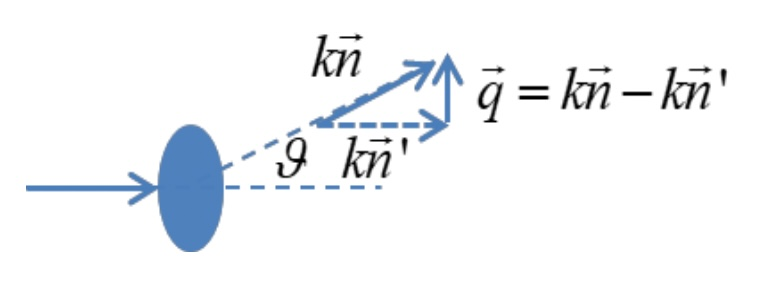
\includegraphics[width = 1.25 \textwidth, height = 1.25 \textheight]{figs/schema-vett-trasferito}
	%    \caption{Sezione d'urto differenziale di una sfera rigida.}
	\label{fig:vett-trasferito}
\end{marginfigure}
otteniamo infine
\[
	k(s+ z') \simeq kr - \bm{q} \cdot \bm{r}'
\]
Se il riferimento è interno alla apertura, a seguito della condizione
di Fraunhofer si ha (sistema \(\simeq\) al centro del foro)
\[
	s \simeq r - \bm{n} \cdot \bm{r'} \simeq r - r' \cos \theta \simeq r
\]
da cui, si ottiene infine l'espressione cercata della \textbf{funzione
d'onda in campo lontano (o di Fraunhofer) scatterata da una apertura $A$
investita da un'onda monocromatica}
\begin{equation}
	\psi(\bm{r}) \simeq - \psi_0 \frac{ik}{2 \pi} \frac{e^{ikr}}{r}
	\iint_{ap A} e^{-i \bm{q} \cdot \bm{r}'}\, da'
	\label{eq:far-field-scattered-wave}
\end{equation}
Come anticipato, però, a noi interessa la situazione complementare,
poiché vogliamo descrivere l'interazione fascio-bersaglio come
diffrazione delle onde di De Broglie del fascio da parte di un ostacolo
avente la forma del bersaglio.

La funzione d'onda \(\psi_{ost A}\) diffratta da uno schermo avente la
forma di A, può essere ottenuta con il semplice \textbf{principio degli
schermi complementari} o \textbf{principio di Babinet.}
\begin{marginfigure}
	\centering
	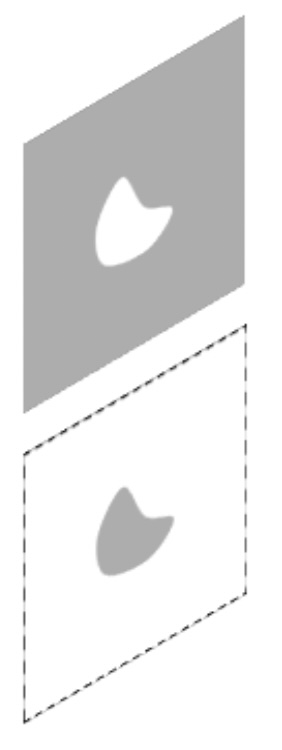
\includegraphics[width = .7 \textwidth, height = .7 \textheight]{figs/kirchhoff-diffraction-3}
	%    \caption{Sezione d'urto differenziale di una sfera rigida.}
	\label{fig:kirchhoff3}
\end{marginfigure}
La (\ref{eq:far-field-scattered-wave}) fornisce la funzione d'onda diffratta dalla apertura $A$ come integrale dei contributi degli elementi d'area
di $A$.
E' chiaro che la funzione d'onda $\psi_{ost A}$, diffratta da uno schermo avente la stessa forma di A, deve essere data
da un integrale dei contributi degli elementi d'area della superficie complementare CA.

Ne consegue che la somma delle funzioni d'onda $\psi_{ap A}+ \psi_{ost A}$ debba essere data da un integrale dei contributi degli elementi d'area del
piano inifinito contenente $A$, integrale che deve restituire l'onda monocromatica piana incidente
\[
	\psi_{ap A}(\bm{r})+ \psi_{ost A}(\bm{r}) = \psi_0 e^{i \bm{k} \cdot \bm{r}}
\]
Da questa relazione possiamo allora ricavare la seguente espressione della \textbf{funzione d'onda diffratta da uno schermo di area A investita da un'onda monocromatica}
\begin{align}
	    \psi_{ost A}(\bm{r}) & =  \psi_0 e^{i \bm{k} \cdot \bm{r}}- \psi_{ap \  A}(\bm{r}) \nonumber \\
		 & \simeq \psi_0 e^{i \bm{k} \
		\cdot \bm{r}} + \psi_0 \frac{e^{ikr}}{r} \frac{ik}{2 \pi} \iint_{A}e^{-i \bm{q} \cdot \bm{r'}} \, da'
		\label{eq:screen-scattered-wave}
\end{align}
All'interno dell'integrale di superficie di questa espressione conviene introdurre la \textbf{funzione di profilo}
$\Gamma$ (nota anche come ``f̀unzione pupilla'' in ottica classica) la quale, nel caso di una apertura A totalmente trasparente, risulta definita nel modo seguente
\[
	\Gamma =
	\begin{cases}
		1   \quad \text{all'interno di } A \\
		0  \quad \text{all'esterno di } A
	\end{cases}
\]
Si ha allora
\[
	\psi_{ost A}(\bm{r}) \simeq \psi_0e^{i \bm{k} \cdot \bm{r}} + \psi_0 \frac{e^{ikr}}{r} \frac{ik}{2 \pi} \iint_{S_B} \Gamma e^{-i \bm{q} \cdot \bm{r'}} \, da'
\]
dove $S_B$ (superficie del bersaglio) è il piano infinito contenente lo schermo/ostacolo $A$.
Si noti che ammettendo valori di $\Gamma$ interni ad $A$ inferiori ad $1$, descriviamo un ostacolo A non più totalmente
assorbente come uno schermo, ma piuttosto parzialmente trasparente: nel caso limite in cui $\Gamma = 0$ abbiamo infatti un ostacolo $A$ totalmente trasparente che non genera alcuna diffrazione e restituisce l'onda piana incidente.

Potremmo ottenere la massima generalità ammettendo che $\Gamma$ possa dipendere dalla posizione $\bm{r}'$ in $A$ ed
\emph{assumere anche valori immaginari in modo da descrivere eventuali effetti assorbitivi}.
Una simile funzione di profilo ci permette di estendere la diffrazione di un ostacolo $A$ totalmente assorbente al caso
generale della diffrazione di un ostacolo $A$ modulante e variamente trasparente, capace di descrivere la diffrazione della funzione d'onda da parte della materia nucleare.
Sulla base di queste considerazioni, la funzione d'onda assume la forma seguente
\begin{marginfigure} Ampiezza di scattering \end{marginfigure}
\[
	\psi_{ost A}(\bm{r}) \simeq \psi_0 e^{i \bm{k} \cdot \bm{r}} + \psi_0 \frac{e^{ikr}}{r} \underbrace{\frac{ik}{2 \pi}
	\iint_{S_B} \Gamma(\bm{r}') e^{-i \bm{q} \cdot \bm{r'}} \, da'}_{f(\bm{q})}
	\qquad \Gamma(\bm{r}') \in \mathbb{C}
\]
Introducendo \textbf{l'ampiezza di scattering}, che integra i contributi modulanti e assorbenti degli elementi d'area dell'ostacolo corrispondenti ad un certo vettore d'onda trasferito $\bm{q}$
\begin{equation}
	f(\bm{q}) = \frac{ik}{2 \pi} \iint_{S_B} \Gamma(\bm{r}')e^{-i \bm{q} \cdot \bm{r}'} \, da'
    \label{eq:scattering-amplitude}
\end{equation}
e da (\ref{eq:screen-scattered-wave}) otteniamo la seguente espressione della \textbf{funzione d'onda in campo lontano diffratta da un ostacolo modulante e assorbente}
\begin{equation}
	\psi_0(\bm{r}) = \psi_0 \left(e^{i \bm{k} \cdot \bm{r}} +
	f(\bm{q}) \frac{e^{ikr}}{r}\right)
	\label{eq:far-field-obstacle-scattered-wave}
\end{equation}
\begin{marginfigure}
	\centering
	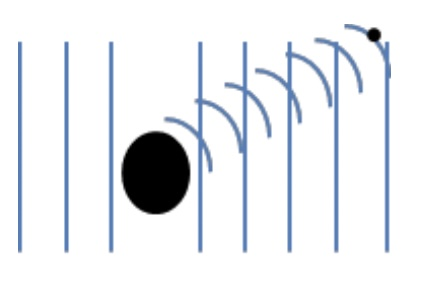
\includegraphics{figs/kirchhoff-diffraction-4}
	%    \caption{Sezione d'urto differenziale di una sfera rigida.}
	\label{fig:kirchhoff4}
\end{marginfigure}
Tale espressione mostra che la figura di diffrazione prodotta da un ostacolo in un dato punto dello spazio è il
risultato della interferenza dell'onda piana incidente con l'onda sferica proveniente dall' ostacolo modulata
dall'ampiezza di scattering.
%%%%%%%%%%%%%%%%%%%%%%%%%%%%%%%%%%%%%%%%%%%%%%%%%%%%%%%%%%%%%%%%%%%%%%%%%%%%%%%%%%%%%%%%%%%%%%%%%%%%%%%%%%%%%%%%%%%%%%%%
%%%%%%%%%%%%%%%%%%%%%%%%%%%%%%%%%%%%%%%%%%%%%%%%%%%%%%%%%%%%%%%%%%%%%%%%%%%%%%%%%%%%%%%%%%%%%%%%%%%%%%%%%%%%%%%%%%%%%%%%
%%%%%%%%%%%%%%%%%%%%%%%%%%%%%%%%%%%%%%%%%%%%%%%%%%%%%%%%%%%%%%%%%%%%%%%%%%%%%%%%%%%%%%%%%%%%%%%%%%%%%%%%%%%%%%%%%%%%%%%%
\section{Le sezioni d'urto in meccanica quantistica}\label{sec:le-sezioni-d'urto-in-meccanica-quantistica}
%%%%%%%%%%%%%%%%%%%%%%%%%%%%%%%%%%%%%%%%%%%%%%%%%%%%%%%%%%%%%%%%%%%%%%%%%%%%%%%%%%%%%%%%%%%%%%%%%%%%%%%%%%%%%%%%%%%%%%%%
%%%%%%%%%%%%%%%%%%%%%%%%%%%%%%%%%%%%%%%%%%%%%%%%%%%%%%%%%%%%%%%%%%%%%%%%%%%%%%%%%%%%%%%%%%%%%%%%%%%%%%%%%%%%%%%%%%%%%%%%
%%%%%%%%%%%%%%%%%%%%%%%%%%%%%%%%%%%%%%%%%%%%%%%%%%%%%%%%%%%%%%%%%%%%%%%%%%%%%%%%%%%%%%%%%%%%%%%%%%%%%%%%%%%%%%%%%%%%%%%%
Per definizone, la \emph{probabilitá che si verifichi una certa ``interazione''} tra fascio e bersaglio corrisponde a
\[
	 p_{int} = \frac{\sigma_{int}}{\Sigma}
\]
un fatto che ci permette di affermare che la sezione d'urto del
processo altro non è che la frazione di sezione del fascio che produce
eventi di quel processo di interazione.
D'altra parte, nella meccanica quantistica, la
probabilità di un certo processo può essere calcolata mettendo a
quoziente il modulo quadrato della funzione d'onda del processo
integrato sulla \emph{superficie di osservazione} $ S_O$ con il modulo
quadrato della funzione d'onda incidente integrata sulla sezione del
fascio \(\Sigma\)\sidenote
{
Si ha una profonda analogia con l'ottica classica. Basti pensare al caso delle onde elettromagnetiche, per cui l'equivalente
della relazione~\ref{eq:quantum-interaction-probability} sarebbe la valutazione del bilancio energetico
tra l'energia dell'onda post processo(scattering/absorption) e quella di quella incidente pre processo.
Il denominatore della ~\ref{eq:quantum-interaction-probability} rappresenta quindi una ``probabilità entrante'',
ovvero il fascio incidente appena prima di interagire con il bersaglio.
}
\begin{equation}
	p_{int}  = \fraclarg{ \iint_{S_O} |\psi_{int}|^2 \, dS}{\iint_{\Sigma} |\psi_{inc}|^2| \, d \Sigma}
	\label{eq:quantum-interaction-probability}
\end{equation}
Il termine a denominatore fa si che sia rispettata la condizione di normalizzazione per cui il quoziente può davvero
rappresentare una probabilità.
Si pensi infatti ai casi limite(per definitezza consideriamo il processo in questione un processo di scattering):
\begin{itemize}
	\item $\psi_{scatt} = \psi_{inc}$: si ha l'onda incidente tutta sullo schermo per cui $ p_{scatt} = 1$;
	misurando sullo schermo tutta l’onda iniziale significa che sicuramente c’è stata l’interazione di
	scattering che ha prodotto l’onda stessa;
	\item $ \psi_{scatt} = 0$: l'interezza dell'onda viene assorbita dallo schermo per cui $ p_{scatt} = 0$.
\end{itemize}
Otteniamo allora la seguente espressione della \textbf{sezione d'urto integrale del processo}
\begin{equation}
	\sigma_{int} = \Sigma \fraclarg{\iint_{S_0} |\psi_{int}|^2 \, dS}{\iint_{\Sigma}|\psi_{inc}|^2 \, d \Sigma}
	\label{eq:integral-interaction-cross-section}
\end{equation}
ed anche quella della \textbf{sezione d'urto elementare del processo}
\begin{equation}
	d \sigma_{int} = \Sigma \fraclarg{|\psi_{scatt}|^2 \, dS}{\iint_{\Sigma}|\psi_{inc}|^2 \, d \Sigma}
	\label{eq:differential-interaction-cross-section}
\end{equation}
dove l'elemento \(dS\) a numeratore si riferisce, come
detto sopra, al generico elemento di superficie di uno schermo lontano
\(S_O\) su cui osserviamo il processo in esame.
%%%TODO 09/12/22 niccolozanotti: Valuta se mettere questa cosa fatta in classe a cazzo di cane
%\marginnote
%{
%	\textbf{Significato fisico della probabilita lungo una superficie(da sistemare)}
%
%	Possiamo vedere la probabilita come qualcosa che fluisce lungo la superficie. Come si scrive un flusso di probabilita su una superficie? Sappiamo gia calcolare quanta probabilita fluisce all'interno di un volume La differenza che sussiste e la stessa che c'e tra densita di carica e densita di corrente \[
%		\nabla \cdot \bm{J} = - \frac{\partial \rho}{\partial t}
%	\] \[
%		\iiint \nabla \cdot \bm{J} \,dV =  - \frac{\partial }{\partial t}\iiint \rho \, dV
%	\] \[
%		\iint_{S(V)} \bm{J}dS = - \frac{\partial }{\partial t}\iiint \rho \, dV  \qquad \bm{j} = \rho \bm{v}
%	\] Questa relazione ci dice: la carica dentro il volume varia in una misura che e uguale al suo flusso di superficie--\> non c'e variazione totale, solo flusso da una parte all'altra--\> cio vale perche le equazioni stabiliscono questo equilibrio
%
%	\[
%		\bm{J} = |\psi|^2\bm{v}
%	\] \[
%		\frac{\iint |\psi_1|^2vds}{\iint |\psi_2|^2vds}
%	\] v e costante essendo in un processo di diffusione.
%}
\bigbreak
Una quantità di interesse nell'analisi di esperimenti di scattering non risulta essere l'onda di scattering stessa ma
piuttosto il rate a cui l'energia è diffusa ed assorbita dall'oggetto.
Si evidenzia un'intima relazione tra il rate di perdita di energia da parte dell'onda incidente a seguito di questi processi
e l'ampiezza dell'onda di scattering nella direzione in avanti(direzione di incidenza).
Questa relazione è quantitativamente espressa dal \textbf{Teorema Ottico} (Optical cross-section theorem) che ora discuteremo.

Nel caso il processo in esame consista nella diffusione da parte dell'ostacolo, risulta possibile calcolare in pochi passaggi la sezione d'urto di scattering nell'angolo solido elementare.
Infatti, dalla (\ref{eq:screen-scattered-wave}) si ottengono subito le seguenti espressioni delle funzioni d'onda incidente e di scattering
\[
	\psi_{inc} = \psi_o e^{i \bm{k} \cdot \bm{r}} \qquad
	\psi_{scatt} = \psi_o f(\bm{q})\frac{e^{ikr}}{r}
\] tenendo poi conto che l'elemento di superficie di un eventuale schermo $S_O$ di forma sferica può essere espresso come segue \[
																																	dS = r^2 d \Omega
\] sostituendo nella (\ref{eq:far-field-obstacle-scattered-wave}) otteniamo
\[
	d \sigma_{scatt} = \Sigma \fraclarg{|\psi_0|^2|f(\bm{q})|^2\frac{1}{r^2}r^2 d \Omega}{\iint_{\Sigma}|\psi_0|^2 \, d \Sigma}
	= \Sigma \frac{|\psi_0|^2|f(\bm{q})|^2 d \Omega}{|\psi_0|^2 \Sigma}
	= |f(\bm{q})|^2 d \Omega
\]
da cui, infine, si derivano le espressioni della \textbf{sezione d'urto di scattering differenziale e totale rispetto all'angolo solido}
\begin{equation}
	\frac{d \sigma_{scatt}}{d \Omega} = |f(\bm{q})|^2 \qquad
	\sigma_{scatt} = \iint_{\Omega}|f(\bm{q})|^2 \, d \Omega
	\label{eq:scattering-cross-section-solid-angle}
\end{equation}

Tale espressione chiarisce che la sezione d'urto differenziale di scattering rispetto all'angolo solido è data dal
modulo quadrato della ampiezza di scattering, dipendente dal vettore d'onda trasferito che parametrizza l'angolo
rispetto alla direzione del fascio.

L' espressione (\ref{eq:screen-scattered-wave}) della funzione d'onda di diffrazione prodotta da un ostacolo ci permette pure il calcolo della sezione d'urto di assorbimento del fascio incidente.
Tale sezione d'urto può essere ottenuta osservando che la probabilità incidente sulla superficie $S_B$ deve essere assorbita dal bersaglio su $S_B$, oppure diffratta e osservata sullo schermo di osservazione $S_O$.
Tenendo presente che la funzione d'onda incidente è non nulla sulla sezione del fascio $\Sigma$, mentre quella di assorbimento è non nulla sul bersaglio, si ottiene la relazione di bilancio:
\begin{gather*}
	\iint_{\Sigma} |\psi_{inc}|^2 \, dS =
	\iint_{S_O} |\psi_{diffr}|^2 \, dS +
	\iint_{bers} |\psi_{ass}|^2 \, d \Sigma\\
	\iint_{\text{bersaglio}} |\psi_{ass}|^2 \, dS =
	\iint_{\Sigma} |\psi_{inc}|^2 \, d\Sigma -
	\iint_{S_O} |\psi_{diffr}|^2 \, dS
\end{gather*}
Da quest'ultima e dalla (\ref{eq:integral-interaction-cross-section}) otteniamo allora la seguente espressione
\[
	\sigma_{ass} =\Sigma \, \fraclarg{\iint_{bers} |\psi_{ass}|^2 \, d \Sigma}{\iint_{\Sigma} |\psi_{inc}|^2 \, d \Sigma}
	= \Sigma \, \fraclarg{\iint_{\Sigma} |\psi_{inc}|^2 \, d\Sigma -
		\iint_{S_O} |\psi_{diffr}|^2 \, dS}{\iint_{\Sigma} |\psi_{inc}|^2 \, d \Sigma}
\]
Se lo schermo di osservazione è sufficientemente lontano e soddisfa la \textbf{condizione di Fraunhofer} possiamo usare la
funzione d'onda diffusa (\ref{eq:far-field-obstacle-scattered-wave}) con asse z normale allo schermo del bersaglio
\begin{align*}
	|\psi_{inc}|^2   & = |\psi_0|^2                                                                                           \\
	|\psi_{diffr}|^2 & = \left | \psi_0 \left( e^{ikz} + f(\bm{q})\frac{e^{ikr}}{r} \right) \right|^2                         \\
	                 & =  |\psi_0|^2 + |\psi_0|^2 \frac{|f(\bm{q})|^2}{r^2} + 2 |\psi_0|^2 \Re f(\bm{q})\frac{e^{ik(r-z)}}{r}
\end{align*}
Integrando sullo schermo si ha\sidenote
{
	Nei conti $ \Sigma^*$ rappresenta la proiezione della sezione del fascio sullo schermo. Se il centro diffusore è piccolo
	(come nel caso di un singolo centro diffusore) gli angoli di scattering sono relativemente piccoli per cui
 possiamo approssimare la proiezione del fascio sullo schermo di osservazione con l’area del fascio incidente.
Ergo $ \Sigma^* \sim \Sigma$
}:
\begin{gather*}
	\iint_{S_O} |\psi_0|^2 \, dS + \iint_{S_O}|\psi_0|^2 |f(\bm{q})|^2\, \frac{dS}{r^2} + \iint_{S_O}2 |\psi_0|^2 \Re f(\bm{q})\frac{e^{ik(r-z)}}{r} \, dS\\
	= |\psi_0|^2 \Sigma^* + |\psi_0|^2 \sigma_{scatt} + 2 |\psi_0|^2 \Re \iint_{S_O} f(\bm{q})\frac{e^{ik(r-z)}}{r} \,dS
\end{gather*}
Per quanto riguarda la sezione d'urto di assorbimento si ha
\[
	\sigma_{ass} = \Sigma   \fraclarg{|\psi_0|^2 \Sigma - \left[ |\psi_0|^2 \Sigma + |\psi_0|^2 \sigma_{scatt} +  2 |\psi_0|^2 \Re \iint_{S_O} f(\bm{q})\frac{e^{ik(r-z)}}{r} \,dS \right]}{|\psi_0|^2 \Sigma}
\]
da cui otteniamo una prima forma della \emph{absoption cross-section}
\begin{equation}
	\sigma_{ass} = - \sigma_{scatt} -  2  \Re \iint_{S_O} f(\bm{q})\frac{e^{ik(r-z)}}{r} \,dS
\end{equation}

Per proseguire negli sviluppi è necessario calcolare l'integrale sullo schermo $S_O$.
Assumendo l'origine del riferimento al centro dell'ostacolo e l'asse z normale al piano che lo contiene e dunque normale anche allo schermo lontano, otteniamo per la fase dell'esponenziale
\begin{marginfigure}
	\centering
	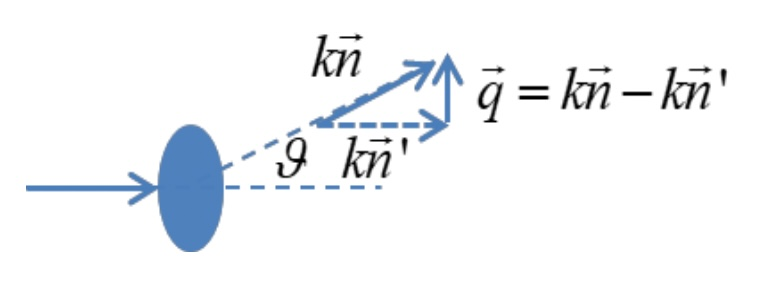
\includegraphics[width = 1.25 \textwidth, height = 1.25 \textheight]{figs/schema-vett-trasferito}
	%    \caption{Sezione d'urto differenziale di una sfera rigida.}
%	\label{fig:vett-trasferito}
\end{marginfigure}
\begin{align*}
	r - z & = \sqrt{x^2 + y^2+z^2} -z = z\sqrt{1 + \frac{x^2}{z^2}+\frac{y^2}{z^2}} -z                       \\
	      & \simeq z \left( 1 + \frac{1}{2}\frac{x^2 + y^2}{z^2}\right) -z  = \frac{1}{2}\frac{x^2 + y^2}{z}
\end{align*}
Inoltre, se lo schermo è lontano la figura di diffrazione si estende sullo schermo stesso in misura trascurabile, per
cui la coordinata $z$ risulta dominare largamente le coordinate $x$ ed $y$.

Risostituendo nell'integrale che compare nell'espressione di $\sigma_{ass}$ abbiamo
\begin{gather*}
	- 2 \Re\iint_{sch}f(\bm{q})\frac{e^{ik(r-z)}}{r} \, dS =
	- 2 \Re f(\bm{o}) \iint_{sch}\frac{e^{ik \frac{x^2 + y^2}{2z}}}{z} \, dxdy\\
	= - \frac{2}{z} \Re f(\bm{o}) \int_{- \infty}^{\infty} e ^{- \frac{k}{2iz}x^2} \, dx
	\int_{- \infty}^{\infty} e ^{- \frac{k}{2iz}y^2} \, dy = - \frac{2}{z} \Re f(\bm{0}) \sqrt{\frac{2iz}{k}}\sqrt{\pi}\sqrt{\frac{2iz}{k}}\sqrt{\pi}\\
	= - \frac{2}{z} \Re f(\bm{0}) \frac{2iz}{k}\pi = - \frac{4 \pi}{k} \Re i (\Re f(\bm{0}) + i  \Im f(\bm{0}))
\end{gather*}
ottenendo infine
\begin{equation}
	\boxed{\sigma_{scatt} + \sigma_{ass} = \frac{4 \pi}{k} \Im f(\bm{0})}
	\label{eq:optical-theorem}
\end{equation}
risultato noto come \textbf{teorema ottico}.
\marginnote{Teorema ottico}

Questo afferma che la somma delle sezioni d'urto totale di scattering ed
assorbimento, detta sezione d'urto totale d'interazione, eguaglia (a
meno del fattore moltiplicativo, $\frac{4 \pi}{k}$, la parte
immaginaria dell'ampiezza di scattering in avanti (ovvero a vettore
d'onda trasferito nullo).
\bigskip

E' importante sapere che le sezioni d'urto totali di scattering e
assorbimento possono essere espresse anche attraverso integrali della
funzione di profilo sulla superficie del bersaglio \(S_B\).
Integrando l'ampiezza di scattering su tutto l'angolo solido nella
(\ref{eq:scattering-cross-section-solid-angle}) si ottiene la seguente espressione della sezione d'urto totale
di scattering in funzione del profilo (vedi Appendice A).
\begin{equation}
	\sigma_{scatt} = \iint_{S_B} |\Gamma(\bm{r}')|^2 \, da'
	\label{eq:scattering-cross-section-profile-func}
\end{equation}
D'altra parte sulla base della (\ref{eq:scattering-amplitude}) il secondo membro del teorema ottico si riscrive come
\begin{align*}
	\frac{4 \pi}{k} \Im[f(\mathbf{0})] &= \frac{4\pi}{k} \Im \frac{ik}{2 \pi} \iint_{S_{B}} \Re \Gamma(\mathbf{r}') +
	i \Im \Gamma(\mathbf{r}') \, da' \\
	& = 2 \Im \iint_{S_{B}} i \Re \Gamma(\mathbf{r}') -  \Im \Gamma(\mathbf{r}') \, da' = \iint_{S_{B}} 2 \Re \Gamma(\mathbf{r}') , da'
\end{align*}
da cui si ottiene la seguente espressione della \textbf{sezione d'urto totale di interazione} in funzione del profilo:
\begin{equation}
	\sigma_{tot} = \iint_{S_{B}} 2 \Re \Gamma(\mathbf{r}') , da'
	\label{eq:total-interaction-cross-section-profile-func}
\end{equation}
Sostituendo la (\ref{eq:scattering-cross-section-profile-func}) e la (\ref{eq:total-interaction-cross-section-profile-func})
nella (\ref{eq:optical-theorem}) otteniamo
\begin{gather*}
    \sigma_{ass} + \iint_{S_B} |\Gamma(\bm{r}')|^2 \, da' = \iint_{S_{B}} 2 \Re \Gamma(\mathbf{r}') , da'\\
    \sigma_{ass} = \iint_{S_{B}} (2 \Re \Gamma(\mathbf{r}') - | \Gamma(\mathbf{r}')|^{2}) \, da'
\end{gather*}
da cui, osservando che
\begin{gather*}
    | 1 - \Gamma|^{2} = (1 - \Re \Gamma)^{2} + (\Im \Gamma)^{2} = 1 + |\Gamma|^{2} - 2 \Re \Gamma\\
    2 \Re \Gamma - | \Gamma |^{2} = 1 - | 1 - \Gamma|^{2}
\end{gather*}
perveniamo infine alla seguente espressione della \textbf{sezione d'urto totale di assorbimento} in funzione del profilo
\begin{equation}
	\sigma_{ass} = \iint_{S_{B}}(1 - | 1 - \Gamma|^{2}) \, da'
	\label{eq:absorption}
\end{equation}
%%%%%%%%%%%%%%%%%%%%%%%%%%%%%%%%%%%%%%%%%%%%%%%%%%%%%%%%%%%%%%%%%%%%%%%%%%%%%%%%%%%%%%%%%%%%%%%%%%%%%%%%%%%%%%%%%%%%%%%%
\section{Diffrazione di un disco assorbente}\label{sec:diffrazione-di-un-disco-assorbente}
%%%%%%%%%%%%%%%%%%%%%%%%%%%%%%%%%%%%%%%%%%%%%%%%%%%%%%%%%%%%%%%%%%%%%%%%%%%%%%%%%%%%%%%%%%%%%%%%%%%%%%%%%%%%%%%%%%%%%%%%

Possiamo usare le formule del precedente paragrafo per calcolare le
sezioni d'urto del processo di \textbf{diffrazione di un'onda piana su
di un ostacolo circolare di raggio R completamente assorbente}.

Adottando un sistema di coordinate polari con l'origine al centro del
disco, la \textbf{funzione di profilo del disco nero} è definita dalle
condizioni
\[
	\Gamma  =
	\begin{cases}
		1  \quad r \leq R \\
		0  \quad r > R
	\end{cases}
\]
Si assuma un riferimento con l'origine al centro del disco e l'asse $z$ normale al piano che lo contiene.
\begin{marginfigure}
	\centering
	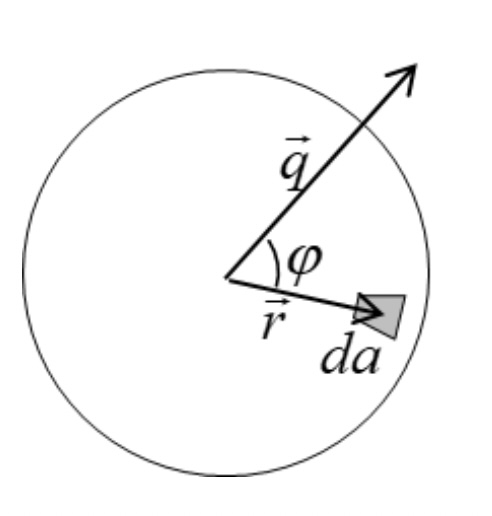
\includegraphics{figs/schema-vett-trasferito-2}
	%    \caption{Sezione d'urto differenziale di una sfera rigida.}
	\label{fig:vett-trasferito2}
\end{marginfigure}
Con questa scelta, se ci limitiamo a considerare angoli di scattering non troppo grandi, il vettore $\bm{q}$ giace in un piano parallelo a al piano $xy$ e si ha \[
	\bm{q} = \bm{k} ( \bm{n} - \bm{n}') = k ( \sin \theta \hat{\imath}_r + \cos \theta \hat{k} - \hat{k'}) \simeq
	k \sin \theta \hat{\imath}_r
\]
il vettore \(\bm{r}\), che identifica i punti del disco circolare (per comodità lasciamo cadere l'accento),
giace sul piano del bersaglio \(xy\) a formare un angolo \(\varphi\) con \(\bm{q}\) per cui si ha
\(\bm{q} \cdot \bm{r} = qr \cos \varphi\),ed infine - adottate le coordinate cilindriche - l'elemento d'area vale
\(da = r d \varphi dr\).

L'ampiezza di scattering (\ref{eq:scattering-amplitude}) si scriverá come
\begin{align*}
	f(\bm{q}) & = \frac{ik}{2 \pi} \int_0^{2 \pi} \int_0^{\infty} \Gamma(r) e^{-iq \cos \varphi r} r \,d \varphi dr                      \\
	& = \frac{ik}{2 \pi} \int_0^R r \left[ \int_0^{2 \pi} e^{-iq \cos \varphi r} d \varphi \right] \, dr                       \\
	& = ik \int_0^R \underbrace{\left[ \frac{1}{2 \pi}\int_0^{2 \pi} e^{-iq \cos \varphi r} d \varphi \right]}_{J_0(qr)} \, dr
\end{align*}
dove \(J_0(qr)\) è nota come \textbf{funzione di Bessel di ordine zero} (vedi Appendice B):
\[
	J_0(qr) = \frac{1}{2 \pi}\int_0^{2 \pi} e^{-iq \cos \varphi r} d \varphi
\]
\begin{marginfigure}
	\centering
	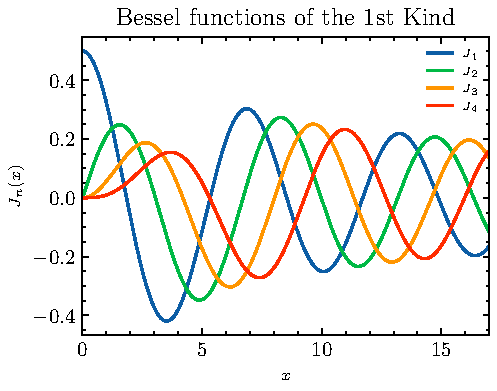
\includegraphics[width = 1.25 \textwidth, height = 1.25 \textheight]{figs/bessel-functions-1stkind}
%	\caption{Rappresentazione grafica delle funzioni di Bessel del primo tipo.}
	\label{fig:bessel-func}
\end{marginfigure}
Abbiamo allora la seguente espressione dell'ampiezza di scattering:
\begin{equation}
	f(\bm{q}) = ik \int_0^R r J_0(qr) \, dr
	\label{eq:scattering-amplitude-bessel-zero}
\end{equation}
che può essere integrata per ottenere (vedi Appendice C)
\[
	f(\bm{q}) = ik \frac{R}{q} J_1(qR)
\]
dove \(J_1(qR)\) è la \textbf{funzione di Bessel di ordine} \(1\).
Tenendo ora conto che \(q = k \sin \theta\) otteniamo infine
\begin{equation}
	f(\bm{q}) = i \frac{R}{\sin \theta} J_1(kR \sin \theta)
	\label{eq:scattering-amplitude-bessel-one}
\end{equation}
%%%TODO 11/12/22 niccolozanotti: discorso su J_1 quando theta -> 0
e da (\ref{eq:scattering-cross-section-solid-angle}) segue l'espressione della \textbf{sezione d'urto differenziale di
scattering del disco assorbente}
\begin{equation}
	\frac{d \sigma_{scatt}}{d \Omega} = \frac{{R}^{2}}{\sin^2 \theta} J_1(kR \sin \theta)
    \label{eq:scattering-differential-cross-section-absorptive-disk}
\end{equation}
Tenendo conto ora della funzione profilo considerata dalla (\ref{eq:scattering-cross-section-profile-func}) si ottiene
la seguente espressione
\[
	\sigma_{scatt} = \iint_{S_B} |\Gamma(\bm{r})|^2 \, da = \iint_{S_B} da
\]
dalla quale segue la \textbf{sezione d'urto totale di scattering del disco assorbente}
\begin{equation}
	\sigma_{scatt} = \pi R^2
	\label{eq:total-scattering-cross-section-absorptive-disk}
\end{equation}
Calcoliamo la forward scattering amplitude:
\[
	f(\bm{0}) = \frac{ik}{2 \pi} \iint_{S_O} \Gamma (\bm{r}) da = \frac{ik}{2 \pi} \iint_{disco} da = \frac{ik}{2 \pi}
	\pi R^2 = i \frac{kR^2}{2}
\] e ricordando il teorema ottico abbiamo
\[
	\sigma_{tot} = \frac{4 \pi}{k} \Im f(\bm{0}) = \frac{4 \pi}{k} \Im \left(i  \frac{kR^2}{2}\right) = \frac{4 \pi}{k}\frac{kR^2}{2}
\]
da segue la \textbf{sezione dl'urto totale d'interazione del disco assorbente}
\begin{equation}
	\sigma_{tot} = 2 \pi R^2
	\label{eq:total-interaction-cross-section-absorptive-disk}
\end{equation}
Dal teorema ottico infine
\[
	\sigma_{ass} = \sigma_{tot} - \sigma_{scatt} = 2\pi ^2 - \pi R^2
\]
da cui segue l'espressione della \textbf{sezione d'urto totale di
assorbimento del disco assorbente}
\begin{equation}
	\sigma_{ass} = \pi R^2
	\label{eq:absorptive-cross-section-absorptive-disk}
\end{equation}

Troviamo allora che la sezione d'urto totale d'interazione di un'onda
piana su di un disco assorbente è il doppio della superficie del disco
stesso, poiché sia la sezione d'urto totale di scattering che quella di
assorbimento hanno entrambe il valore di quella superficie.
%%%%%%%%%%%%%%%%%%%%%%%%%%%%%%%%%%%%%%%%%%%%%%%%%%%%%%%%%%%%%%%%%%%%%%%%%%%%%%%%%%%%%%%%%%%%%%%%%%%%%%%%%%%%%%%%%%%%%%%%
\section{Il raggio nucleare}\label{sec:raggio-nucleare}
%%%%%%%%%%%%%%%%%%%%%%%%%%%%%%%%%%%%%%%%%%%%%%%%%%%%%%%%%%%%%%%%%%%%%%%%%%%%%%%%%%%%%%%%%%%%%%%%%%%%%%%%%%%%%%%%%%%%%%%%
Nell'ottica, forma, dimensioni ed altre proprietà di un oggetto possono
essere studiate inviando su di esso onde luminose e registrando le onde
emergenti su di uno schermo. Scegliendo la lunghezza d'onda della luce
in modo da avere il potere risolutivo desiderato, sullo schermo apparirà
una figura di diffrazione con una distribuzione dell'intensità luminosa
che caratterizza l'oggetto illuminato. Data l'onda incidente quindi, il
problema sarà quello di risalire dalla distribuzione della intensità
luminosa osservata alle proprietà dell'oggetto illuminato.

In fisica nucleare e subnucleare le cose vanno esattamente nello stesso modo.
L’oggetto da studiare può essere un nucleo oppure - se si dispone di sufficiente potere risolutivo (ovvero di un fascio di sufficiente energia) - un nucleone o addirittura una sua parte.
Tale oggetto potrà essere illuminato non solo con fasci di luce (tipicamente nella regione dei raggi X e gamma) ma anche con fasci di ‘onde materiali’ (nel senso di De Broglie) di elettroni, protoni, neutroni ed altre particelle ancora, con le quali è in generale più facile ottenere piccole lunghezze d’onda e dunque elevate risoluzioni.
Le ‘onde materiali’ emergenti potranno essere registrate come ‘particelle’ da superfici sensibili (rivelatori), distribuite spazialmente in un modo caratteristico dipendente dalle proprietà dell’oggetto illuminato.

Ciò premesso, i ragionamenti che potrebbero guidare un esperimento per
la \textbf{misura delle dimensioni del nucleo atomico} sono i seguenti:
\begin{enumerate}
	\tightlist
	\item
	\emph{Scelta delle particelle del fascio}. L'uso di fasci di elettroni
	permetterebbe di ottenere dati molto precisi sia per la qualità dei
	fasci disponibili che per la puntiformità delle particelle e
	l'eccellente conoscenza teorica della interazione elettromagnetica. E'
	però chiaro che gli elettroni restituirebbero una `radiografia' della
	distribuzione nucleare dei soli protoni. Volendo ottenere informazioni
	sulla distribuzione di tutti i nucleoni sarebbe meglio utilizzare
	fasci di \emph{neutroni} i quali - interagendo solo fortemente -
	`vedrebbero' sia i protoni che i neutroni senza il `disturbo'
	addizionale della interazione elettromagnetica che invece si avrebbe
	usando fasci di \emph{protoni}. Tali vantaggi competono però con la
	qualità inevitabilmente inferiore dei fasci di neutroni;
	\item
	\emph{Scelta della energia del fascio}. La scelta della energia è
	essenzialmente dettata dal potere risolutivo che si vuole avere nello
	studio della struttura del nucleo per cui la lunghezza d'onda di De
	Broglie delle particelle del fascio deve essere almeno dell'ordine di
	grandezza delle dimensioni nucleari. Nel caso dei neutroni, si avrebbe
	una risoluzione dell'ordine di \(10 \  fm \,(1 fm=10^{-15} m)\) con
	circa 10 MeV di energia cinetica
	\[
		\lambda \simeq 10 fm \simeq 10 \frac{1}{200} \frac{\hbar c}{MeV} \simeq \frac{1}{20} \frac{\hbar  c}{MeV}
	\]
	Sfruttando ora il fatto che $v \ll c$ si ha
	\begin{gather*}
	    E_{cin} = \sqrt{ p^{2}c^{2}+m^{2}c^4 } - mc^{2} \simeq mc^{2} \left(1 + \frac{1}{2} \frac{{p^{2}c^{2}}}{m^{2}c^4}- mc^{2}\right) \simeq \frac{p^{2}}{2m} \simeq \frac{\hbar^{2}k^{2}}{2m}\\
	    \simeq 2\pi^{2} \frac{\hbar c^{2}}{mc^{2}\lambda^{2}} \simeq 20 \frac{\hbar^{2} c^{2} }{1000MeV_{1}} \frac{1}{400} \frac{\hbar^{2} c^{2}}{MeV^2} \simeq 8 MeV
	\end{gather*}
	\item
	\emph{Processi in gioco}. Difficilmente un esperimento può prescindere
	da una qualche ipotesi/conoscenza dei processi che avranno luogo nelle
	condizioni scelte. \textbf{Assumendo che i neutroni da \(10 \ MeV\) non
	riescano a trapassare il nucleo atomico, questo potrà essere
	assimilato ad un disco assorbente}.
\end{enumerate}

Sulla base di queste considerazioni si potrà costruire un esperimento
per determinare il raggio nucleare, attraverso la misura delle sezioni
d'urto totali e di scattering di neutroni su bersagli materiali.
Ipotizzando che il nucleo possa essere descritto da un disco assorbente
si ha la seguente espressione della sezione d'urto totale (\ref{eq:total-interaction-cross-section-absorptive-disk})
\[
	\sigma = 2 \pi R^2
\]
Si possono allora determinare i raggi nucleari misurando la sezione
d'urto totale di neutroni di circa 10 MeV su bersagli materiali puri
contenenti i diversi tipi di nucleo.
Dato che sia le interazioni elastiche che inelastiche rimuovono i neutroni del fascio, la sezione d'urto totale di
interazione potrà essere misurata contanto i neutroni persi dal fascio stesso.
In figura~\ref{fig:cross-section-neutroni} è mostrato un grafico della \textbf{sezione d'urto totale e
di assorbimento} di neutroni da 14 MeV in funzione della radice cubica
del numero di nucleoni A del nucleo.
\begin{figure}
	\centering
	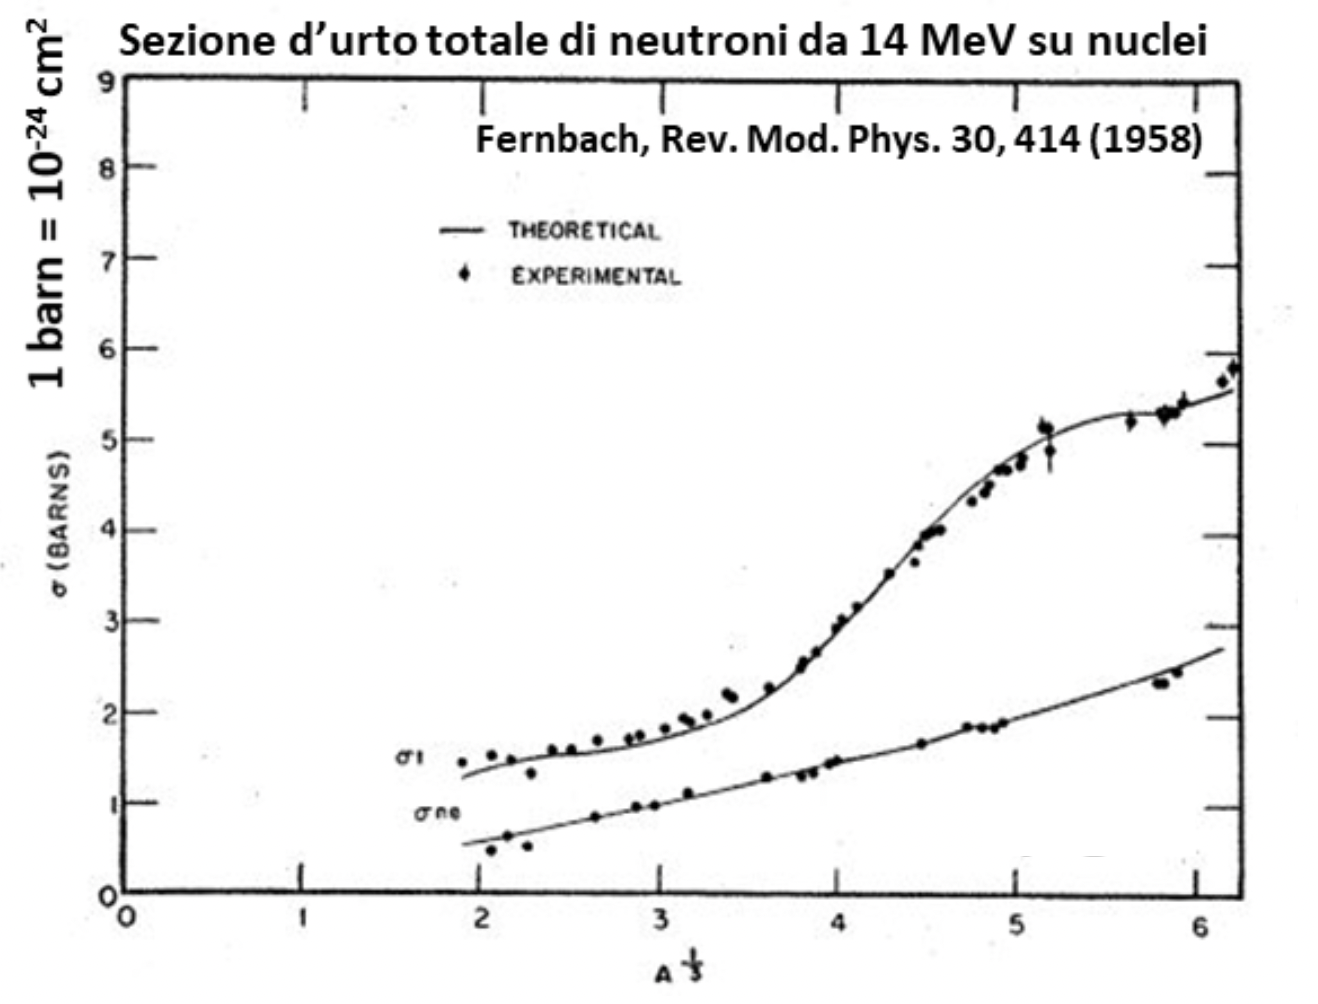
\includegraphics{figs/grafico-cross-sect-neutroni}
	\caption{Sezione d'urto totale di neutroni da $14$ MeV su nuclei.}
	\label{fig:cross-section-neutroni}
\end{figure}

Ci serve un modello capace di fornire una relazione tra la sezione d'urto totale ed il numero di nucleoni del nucleo.
Per cominciare, potremmo modellizzare il nucleo come un \textbf{aggregato sferico di nucleoni} a loro volta assimilati a piccole sfere.
Ipotizzando che la forza che lega neutroni e protoni sia a \textbf{corto raggio} con raggio d'azione dell'ordine delle dimensioni del singolo nucleone, il nucleo tenderà ad avere una \textbf{densità volumetrica uniforme} per cui potremo scrivere le seguenti relazioni \[
	V_{Nuc} \simeq \frac{4}{3} \pi R^3 \qquad V_{Nuc} \simeq A\frac{4}{3} \pi {r_{0}}^3
\] dalle quali si ottiene la seguente relazione tra raggio nucleare e numero atomico
\[
	R \simeq r_{0} A^{1/3}
\]
Immaginando ora il nucleo come un disco assorbente, possiamo sostituire questa relazione nella (\ref{eq:total-interaction-cross-section-absorptive-disk}) ed ottenere la seguente formula con la quale interpretare i dati \[
	\sigma = 2 \pi r_{0}^{2}(A^{1/3})^{2}
\]
In prima approssimazione la formula funziona.
Si noti infatti che i dati hanno effettivamente un andamento ad arco di parabola nella variabile $A^{1/3}$ ma, contrariamente alla previsione della formula, intersecano l'asse verticale ($A=0$) ad un valore di sezione d'urto non nullo.
Ciò significa che dobbiamo aggiungere un termine costante alla sezione d'urto di cui sopra ottenibile solo con l'aggiunta di un termine costante nella espressione del raggio nucleare
\begin{equation}
	R_{Nuc} = r_{0} A^{1/3} + b
	\label{eq:nuclear-radius-skin}
\end{equation}
Hans Bethe suggerì che tale termine dovesse interpretarsi come un una specie di \textbf{'alone nucleare'(nuclear skin), di spessore costante ed uguale per tutti nuclei, dovuto al raggio finito della interazione forte tra nucleoni.} Stimando in circa $0.5$ barn
il valore approssimativo della sezione d'urto totale ad $A=0$ possiamo estrarre la corrispondente stima di $b$
\begin{gather*}
    \sigma = 2 \pi R^{2} = 2 \pi (r_{0} A^{1/3} +b)^{2} \quad \sigma(A^{1/3}=0) = 2\pi b^{2}\\
    b = \sqrt{ \frac{\sigma(A^{1/3}=0)}{2 \pi} }\sim 2.8 \ \text{fm}
\end{gather*}
Il valore meglio compatibile con i dati sperimentali oggi disponibili è circa $b=2.4 \, fm$.
Una volta determinata la `skin' nucleare possiamo determinare anche il raggio del nucleone $r_0$.

Leggendo il valore della sezione d'urto totale d'interazione corrispondente ad un secondo nucleo (ad esempio $A^{1/3}=4$ dove $\sigma = 2.8$ barn)
possiamo ottenere la seguente stima di $\bm{r_0}$
\begin{gather*}
	\sigma = 2 \pi R^2 = 2 \pi (r_0 A^{1/3} +b)^2  \qquad r_0 = \frac{1}{A^{1/3}} \left( \sqrt{\frac{\sigma}{2 \pi}}-b \right)\\
	r_0 \simeq \frac{1}{4} \left( \sqrt{\frac{2.8 \times 10^{-24}}{2 \pi} } - 2.4 \times 10^{-13} \right) \simeq1.1 \ fm
\end{gather*}
Il valore meglio compatibile con i dati sperimentali oggi disponibili fornisce $ \bm{r}_0 = 1.24$.
In sintesi, dato il numero di nucleoni $ A$, la (\ref{eq:nuclear-radius-skin}) - completata dai valori sperimentali della
skin nucleare e del raggio del nucleone - permette di calcolare in modo preciso \textbf{il raggio dei nuclei nello stato
fondamentale di minima energia dove il nucleo assume una forma sferica}.

Informazioni più dettagliate sulla geometria del nucleo possono essere ottenute da esperimenti capaci di misurare
la sezione d'urto differenziale di scattering.
Modellizzando il \emph{nucleo come un disco circolare assorbente} (vedi assunzione fatta sui processi in gioco)
la una sezione d'urto differenziale di scattering sarà data dalla espressione (\ref{eq:scattering-differential-cross-section-absorptive-disk})
\[
	\frac{d\sigma_{scatt}}{d \Omega} = \frac{R^{2}}{\sin ^{2}\theta}J_{1}^{2}\left( \frac{2 \pi R}{\lambda} \sin \theta \right)
\]
che va confrontata con i dati sperimentali mostrati a fianco.
\begin{marginfigure}
	\centering
	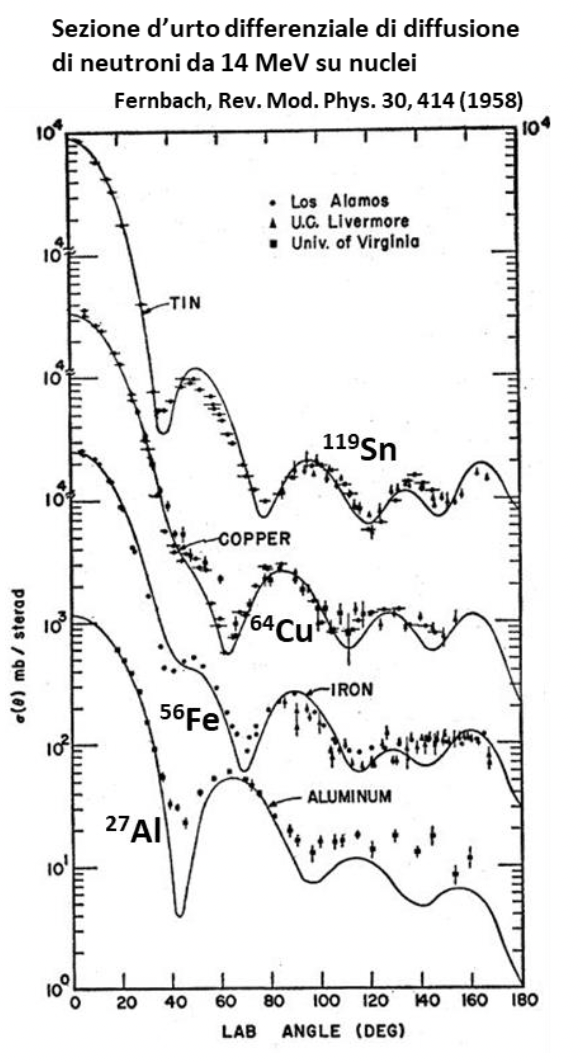
\includegraphics[width = 1.25 \textwidth,height = 1.25 \textheight]{figs/grafico-cross-sect-neutroni-2}
	%    \caption{Sezione d'urto differenziale di una sfera rigida.}
	\label{fig:cross-section-neutroni2}
\end{marginfigure}
Si nota subito che i dati mostrano un andamento con l'angolo $\theta$ di tipo diffrattivo, in prima approssimazione
compatibile con quello di una funzione di Bessel del primo ordine.

È interessante considerare la sezione d'urto differenziale in avanti, ovvero per $\theta$ prossimo a zero.
Sviluppando asintoticamente la funzione di Bessel per piccoli valori dell'argomento si ha(9.4.4 Abramowitz-Stegun\cite{AbramSteg})
\[
	J_{1}(z) \sim \frac{1}{2}z - \frac{1}{16}z^{3}
\]
da cui - sostituendo - otteniamo la \textbf{sezione d'urto differenziale di scattering in avanti} dalla quale si può ottenere una nuova \textbf{stima del raggio nucleare}
\[
	\frac{d\sigma_{scatt}}{d \Omega} = \frac{R^{2}}{\sin ^{2}\theta}J_{1}^{2}\left( \frac{2 \pi R}{\lambda} \sin \theta \right) \sim \frac{R^{2}}{\sin ^{2}\theta} \frac{1}{4} \frac{4 \pi^{2} R^{2}}{\lambda^{2}} \sin ^{2} \theta \sim \frac{\pi^{2}R^{4}}{\lambda^{2}}
\]
Dalla figura si vede chiaramente che tale sezione d'urto a $\theta=0$ aumenta rapidamente con il numero di nucleoni $A$.

A titolo di esempio potremmo determinare il raggio nucleare leggendo sul grafico il valore della sezione d'urto sul picco di
diffrazione.
Calcolando la lunghezza d'onda di De Broglie dei neutroni del fascio:
\[
 E = \frac{{p}^{2}}{2m} = \frac{2 \pi^2 \hslash^2}{m \lambda^2} \quadd
 \lambda = \sqrt{\frac{2 \pi^2}{m c^2 E}} \hslash c = 7.5 \, fm
\]
nel caso del \textbf{picco centrale di diffrazione dell'alluminio} si ottiene
\[
 R = \sqrt[4]{\frac{\lambda^2}{\pi^2} \frac{d \sigma}{d \Omega}} = 5.2 \, fm
\]

Una seconda possibilità consiste nel lavorare sui minimi di diffrazione la cui spaziatura - come noto dall'ottica - deve dipendere dal raggio del disco ovvero dal raggio nucleare.
Notiamo subito che l’andamento della sezione d’urto di diffusione per angoli non nulli dovrebbe essere governato dal quadrato della funzione di Bessel del primo ordine.
Ora è noto che le funzioni di Bessel si annullano ripetutamente, un fatto che però non trova corrispondenza nell’andamento
delle sezioni d’urto di diffuzione misurate che, pur avendo dei minimi pronunciati, non si annullano mai (vedi figura).
Questo fatto indica che \emph{modellizzare il nucleo come un disco completamente assorbente non è del tutto appropriato e che esiste un certo grado di trasparenza del nucleo rispetto ai neutroni incidenti}.
Trascurando per ora questo fatto ed assumendo che i minimi della sezione d’urto corrispondano agli zeri della funzione di Bessel, abbiamo nel caso del primo zero (9.5.14 Abramowitz-Stegun)
\[
	J_{1}\left( \frac{2 \pi R}{\lambda}\sin \theta \right) = 0  \quad \text{se}
	\quad \frac{2 \pi R}{\lambda}\sin \theta = 3.832
\]
da cui si ottiene la seguente espressione
\[
	R = \frac{3.832}{2 \pi} \frac{\lambda}{\sin \theta}
\] che fornisce un'altra \emph{stima del raggio nucleare} a partire dalla posizione angolare del primo minimo della
sezione d'urto differenziale di scattering.

Posizionandoci sul primo minimo di diffrazione dell’alluminio - molto marcato - otteniamo il valore seguente
\[
 R = \frac{3.832 \lambda}{2 \pi \sin \theta} = 6.12 \, fm
\]
in ottimo accordo con la stima ottenuta dalla (\ref{eq:nuclear-radius-skin})
\[
      R_{Nuc} = r_0 A^{1/3} + b \simeq 6.12 \, fm 
\]
La lettura diretta dei dati che abbiamo commentato è solo un modo per prendere confidenza con i dati stessi.
Per estrarne in modo corretto tutto il contenuto informativo, sarebbe necessario eseguire un ‘fit’ utilizzando il corrispondente chi-quadrato come criterio di bontà e affidabilità della funzione teorica adottata.
In questo modo otterremmo un solo valore del raggio nucleare piuttosto che i due stimati e, soprattutto,
verificheremmo che l’ipotesi che il nucleo assorba totalmente i neutroni incidenti è troppo drastica poiché non riesce a riprodurre correttamente l’andamento delle sezioni d’urto di diffusione.
I dati richiedono l’ipotesi che il nucleo sia parzialmente trasmittente un po’ come accade alla luce incidente su di una sfera di vetro solo parzialmente opaca.
Dato che nel caso della luce si descriverebbe un simile comportamento per mezzo di un indice di rifrazione dotato sia di
una parte reale che immaginaria, si è pensato di modellizzare il nucleo per mezzo di un potenziale complesso (dotato sia
di una parte reale che immaginaria) dando origine al cosiddetto \textbf{modello ottico del nucleo}\sidenote{
	Description of atomic nuclei as similar to cloudy crystal balls in that, when struck by a beam of particles,
	they partially absorb the beam, partially scatter it, and partially transmit it in a way analogous to the behaviour
	of light. The nuclear optical model has proved very successful in explaining nuclear reactions in which the incident
	(striking) particles have energies of about $10^6$ to $10^9$ eV.
}, capace di descrivere
perfettamente i dati sperimentali disponibili (la parte reale del potenziale è solitamente assunta nella forma di
Saxon-Woods mentre quella immaginaria nella forma di una gaussiana).
%%%%%%%%%%%%%%%%%%%%%%%%%%%%%%%%%%%%%%%%%%%%%%%%%%%%%%%%%%%%%%%%%%%%%%%%%%%%%%%%%%%%%%%%%%%%%%%%%%%%%%%%%%%%%%%%%%%%%%%%
\section{Energia di legame nucleare}\label{sec:energia-di-legame-nucleare}
%%%%%%%%%%%%%%%%%%%%%%%%%%%%%%%%%%%%%%%%%%%%%%%%%%%%%%%%%%%%%%%%%%%%%%%%%%%%%%%%%%%%%%%%%%%%%%%%%%%%%%%%%%%%%%%%%%%%%%%%
Importanti indicazioni sulle proprietà della forza nucleare che unisce i nucleoni nel nucleo provengono dalle misure sperimentali
della \textbf{energia di legame} compiute in modo sistematico a partire dagli anni ’20.
Introduciamo ora il concetto di energia di legame del nucleo per mezzo di un semplice esempio.

Si immagini un sistema formato da due sferette omogenee di massa m e raggio $R$, soggette alla mutua attrazione gravitazionale, disposte in quiete l'una accanto all'altra con una energia potenziale iniziale $E_{i}$.
Sappiamo che per separare le sferette dobbiamo applicare su una di esse una forza esterna uguale e contraria a quella attrattiva in modo da portarla all'infinito (avendo avuto cura di fissare l'altra!).
Nel linguaggio della meccanica dobbiamo compiere lavoro contro la forza attrattiva gravitazionale che tiene unite le sferette, nel più generale linguaggio della energia dobbiamo fornire energia al sistema legato in modo da separarlo nei suoi componenti portandolo ad una energia potenziale finale che indicheremo con $E_{f}$ (in questo caso nulla).
Tale energia viene detta \textbf{energia di legame del sistema} e soddisfa la seguente relazione
\begin{marginfigure}
	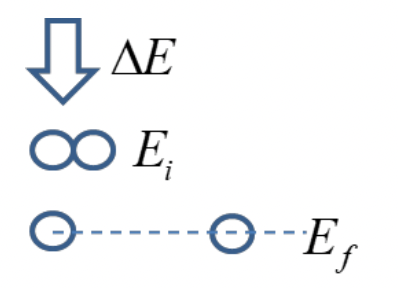
\includegraphics{figs/en-legame}
	%    \caption{Sezione d'urto differenziale di una sfera rigida.}
	\label{fig:en-legame}
\end{marginfigure}

\begin{equation}
	\Delta E = E_{i} = E_{f}
	\label{eq:binding-energy-experimental}
\end{equation}
Ora immaginiamo di volerla determinare.
In linea di principio potremmo utilizzare \textbf{tre diversi metodi}:
\begin{enumerate}
	\tightlist
	\item Disponendo di una espressione esplicita della forza, potremmo
	calcolarla teoricamente
	\[
		\Delta E = \int_{2 R}^{\infty} \bm{F}_{est} \cdot d\bm{l} = \int_{2 R}^{\infty} G \frac{m^{2}}{r^{2}} \, dr
		= G \frac{m^{2}}{2R}
	\]
	\item
	Non disponendo della espressione teorica potremmo misurare
	ripetutamente la forza applicata sulla sferetta e sommare in modo da
	ottenere il lavoro compiuto
	\[
		\Delta E = \int _{2R}^{\infty} \bm{F}_{est} \cdot d\bm{l}
	\]
	\item
	Non disponendo della espressione teorica potremmo anche affidarci alla
	teoria della relatività ristretta (TRR).
	Sappiamo infatti che ad ogni forma di energia $E$ corrisponde una massa inerziale equivalente
	\(M\) data dalla ben nota equazione \(M=E/c^{2}\).
	Su questa base,dato che il contenuto energetico del sistema iniziale legato e del
	sistema finale separato sono diversi, dobbiamo aspettarci che diverse
	siano pure le corrispondenti masse inerziali. In particolare da
	\(\Delta E = E_{i} = E_{f}\) otteniamo \(E_{f} > E_{i}\) (poiché
	\(\Delta E >0\)) da cui discende pure che \(M_{f} > M_{i}\) .
	Dalle espressioni relativistiche
	\[
		E_{f} = M_{f}c^{2} \qquad E_{i} = M_{i}c^{2}
	\] otteniamo allora la seguente differenza di massa detta
	\textbf{difetto di massa del sistema legato}
	\[
		(M_{f}-M_{i}) = \frac{\Delta E}{c^{2}}
	\] la quale offre una terza via per accedere all'energia di legame.
\end{enumerate}

Nel caso di un sistema macroscopico di due masse legate dalla forza
gravitazionale, il metodo \(1\) risulta praticabile poiché conosciamo
l'espressione teorica della forza. Superando un certo numero di
difficoltà sperimentali potremmo anche utilizzare il metodo \(2.\)
Certamente nessun fisico sperimentale sarebbe però in grado di
utilizzare il metodo \(3\) dato che dovrebbe misurare il seguente
difetto di massa
\[
	(M_{f}-M_{i}) = \frac{\Delta E}{c^{2}} = G \frac{m^{2}}{2Rc^{2}} = 5.6 \times 10^{-54} MeV
\]
Nel caso della interazione forte tra nucleoni le cose vanno
diversamente. Il metodo \(1\) richiederebbe una conoscenza della forte
che non abbiamo poiché - appunto - dobbiamo ancora determinarne le
proprietà. Il metodo \(2\) è chiaramente inapplicabile ad un sistema
microscopico. Il metodo \(3\), basato sulla TRR, potrebbe essere
applicabile qualora il difetto di massa del sistema fosse consistente.
Ora i dati sperimentali mostrano che \textbf{l'energia potenziale
dell'interazione attrattiva tra nucleoni è tale da fornire un
apprezzabile contributo negativo alla inerzia del nucleo}, generando una
differenza misurabile tra la massa dei nucleoni componenti e quella del
nucleo stesso.

Sulla base di quanto detto, siamo ora in grado di fornire la seguente
\textbf{definizione operativa della energia di legame} ovvero della
\emph{energia necessaria per separare il nucleo nei nucleoni componenti}
\begin{equation}
	B \left( {\isotope[A][Z]{\mathlarger{X}_{N}} \right)  = \left[ Nm_{n} + Zm_{p} -m_{N}
	\left( \isotope[A][Z]{\mathlarger{X}_{N}} \right) \right] c^{2}
	\label{eq:binding-energy-definition}
\end{equation}
dove $m_{n},m_{p},m_{N}$ sono rispettivamente le masse del neutrone, del protone e del nucleo\sidenote{
	Vale la pena precisare che le masse nucleari sono misurabili con minore precisione di quelle atomiche per cui è utile ricavare le prime delle seconde attraverso la relazione \[
	m_{A}\left( \isotope[A][Z]{\mathlarger{X}_{N}} \right) = m_{N}\left( \isotope[A][Z]{\mathlarger{X}_{N}} \right)+Zm_{e}
	- \frac{1}{c^{2}}\sum_{i = 1}^{Z}B_{i}^{el}
\] dove $m_{A}$ è la massa dell'atomo corrispondendente al nucleo in esame.}.
La formula (\ref{eq:binding-energy-definition}), attraverso la misura sistematica delle masse nucleari, rende possibile la determinazione dell’energia
di legame dei nuclidi che può essere tabulata in funzione di una qualunque coppia tra le variabili A, Z ed N (vedi \ref{sec:le-carte-dei-nuclidi}).
Limitando la rappresentazione ai soli nuclidi stabili (nel caso vi fosse più di un isotopo
stabile si sceglie quello più abbondante) si ottiene l’energia di legame media per nucleone B/A in funzione di A riportata
in Figura~\ref{fig:binding-energy-stable} e riportata nella pagina seguente.
Il quoziente B/A da una indicazione quantitativa del grado di stabilità del nuclide e permette di stabilire se una data reazione nucleare sia esoenergetica o endoenergetica e, dunque, se possa avvenire spontaneamente oppure no.
\begin{figure}
	\centering
	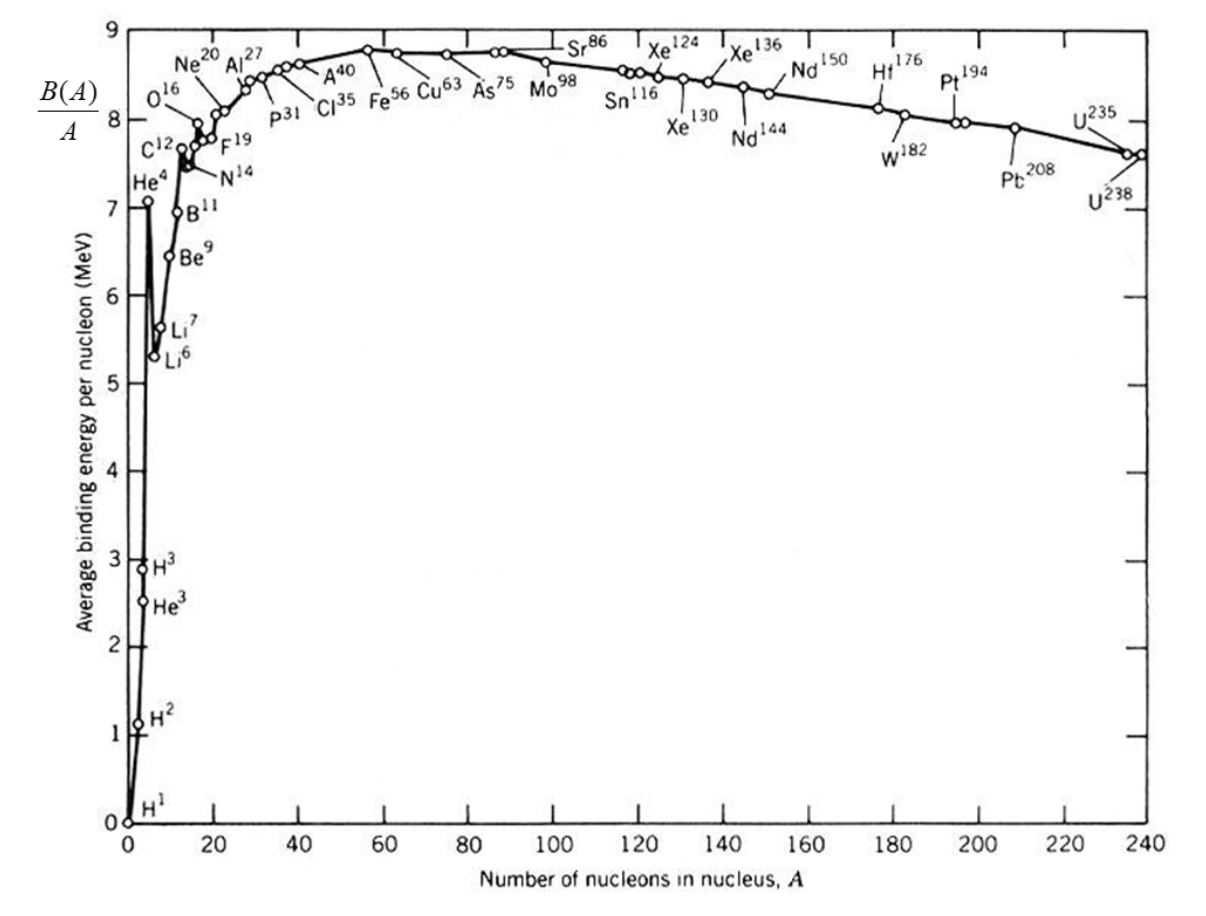
\includegraphics{figs/en-legame-graph}
	\caption{Grafico dell'energia di legame media per nucleone in funzione del numero di nucleoni $A$.}
	\label{fig:en-legame-graph}
\end{figure}
Dal grafico in figura~\ref{fig:en-legame-graph} possiamo trarre alcune conclusioni generali:
\begin{enumerate}
	\item Ci sono configurazioni nucleari particolarmente stabili quali ${}^{4}He, {}^{12}_{}C, {}^{16}_{}O, \dots$
	\item a parte queste eccezioni, l'energia di legame media per nucleone ha un andamento regolare.
	      Aumenta rapidamente con il numero di nucleoni fino ad un valore dell'ordine degli $8 \ MeV$ per poi diminuire assai lentamente
	\item i nucleo piu stabili sono ${}^{56}_{}Fe$ e ${}^{62}_{}Ni$.
	Ciò significa che i nuclei pesanti alla sua destra possono raggiungere configurazioni più stabili ($B/A$ più elevato) diminuendo il numero di nucleoni A, ovvero frazionandosi in nuclei più piccoli.
	Mentre i nuclei leggeri alla sua sinistra possono raggiungere configurazioni più stabili ($B/A$ più elevato) aumentando A, ovvero aggregandosi in nuclei più grandi.
	Detto in altri termini ciò significa che le \textbf{reazioni di fissione dei nuclei pesanti e e quelle di fusione dei nuclei
	leggeri sono esoenergetiche} ovvero producono energia qualora si sia in grado di innescarle;
	\item dal punto precedente consegue che \textbf{le reazioni di fusione dei nuclei leggeri e fissione dei nuclei pesanti} costituiscono la doppia opportunità offerta dalla fisica nucleare per la produzione di energia.
\end{enumerate}

La via della \emph{fusione nucleare} è stata scelta dalle stelle.
Oggi sappiamo che una stella come il sole ricava la quasi totalità della energia
(circa il \(98 \%\)) dalla fusione di nuclei d'idrogeno in nuclei di
elio.
L'energia prodotta dalle reazioni di fusione fluisce verso
l'esterno.
Tale flusso, nella forma di energia cinetica dei prodotti
delle reazioni di fusione, fornisce la spinta verso l'esterno capace di
opporsi alla contrazione gravitazionale mantenendo il sole in una
situazione di equilibrio di forze detto equilibrio idrostatico\sidenote
{
I fisici delle particelle elemtnari trovano naturale misurare le masse atmoiche e nucleare in unita di $ eV/c^2$
ma, i fisici nucleari e soprattutto i chimici, biochimici, e i biologi molecolari preferiscono usare una scala di
massa la cui unità è prossima a quella del protone e del neutrone.
Si tratta della \textbf{unità di massa atomica} (simbolo \textbf{u}) definita come \textbf{la dodicesima parte della massa
dell'atomo di carbonio-12}.
È evidente che tale unità di massa, a causa dell'inerzia negativa associata all'energia di legame del nucleo deve essere
inferiore sia alla massa del protone che a quella del neutrone:
\[
   \frac{1}{12} M_A (\isotope[12][6]{\mathlarger{C}}) = \frac{1}{12} \left[M_N \isotope[12][6]{\mathlarger{C}} + 6 m_e -
	\frac{1}{{c}^{2}} \sum_{i = 1 }^{6} B_i^{e^-} \right]
\]
\[
	= \left[\frac{1}{12} 6 m_n + 6 m_p - \frac{1}{{c}^{2}} \sum_{i = 1 }^{12} B_i^{nucl} + 6 m_e -
	\frac{1}{{c}^{2}} \sum_{i = 1 }^{6} B_i^{e^-}\right]
\]
\[
	\simeq \frac{m_n + m_p + m_e}{2} - \frac{1}{12} \sum_{i = 1 }^{12} \frac{B_i^{nucl} }{{c}^{2}}
	\simeq 931.5 MeV
\]
Infatti la conversione tra $u$ e MeV/$c^2$ è ovvero $ 1 \%$ inferiore alla massa del neutrone e del protone.
}.

Dal grafico si può leggere il decorso del processo una volta esaurito
l'idrogeno: la contrazione gravitazionale prenderà il sopravvento
comprimendo la materia fino al punto da innescare le reazioni di fusione
di tre nuclei di elio in un nucleo di carbonio stabilendo un nuovo
periodo di equilibrio.
Le fasi di equilibrio e contrazione si
alterneranno fino alla fusione del silicio in ferro quando la
contrazione gravitazionale - non potendo innescare altre reazioni di
fusione - procederà inarrestabile facendo collassare la stella che
espellerà in modo esplosivo gli strati più esterni lasciando un residuo
compatto di materia in uno stato degenere.

La via della \emph{fissione nucleare} trova invece una sua applicazione
nei reattori nucleari.
Alcuni nuclidi detti \emph{fissili}– quali ad esempio l'$ \isotope[235][92]{\mathlarger{U}}$
ed il $ \isotope[239][94]{\mathlarger{Pu}}$ - possiedono elevate sezioni d’urto di cattura di neutroni termici
(neutroni con energie dell’ordine di 0.03 eV, comparabili con quella di agitazione termica a temperatura ambiente) e,
a seguito della cattura neutronica, tendono a spezzarsi in due nuclei leggeri più alcuni neutroni liberi di
qualche MeV di energia.

E’chiaro che irradiando con neutroni termici un \emph{nocciolo materiale} contenente materiale fissile, la elevata
energia cinetica (quasi 200 MeV) dei nuclidi prodotti dalla fissione diffonderà all’esterno come \emph{calore} asportato
da un \emph{fluido refrigerante} mentre i \emph{neutroni liberi} potranno indurre ulteriori reazioni di fissione del
materiale dando luogo ad una \emph{reazione a catena}.
Come detto però, affinchè ciò avvenga in misura sufficiente, è necessario abbassare l’energia di tali neutroni liberi
da qualche Mev al livello termico, funzione cui provvede il \emph{materiale moderatore}.
Fondamentale è poi la possibilità di controllare la rapidità di sviluppo delle reazioni a catena che solitamente viene
ottenuta inserendo o togliendo dal nocciolo apposite \emph{barre di controllo} capaci di assorbire i neutroni prodotti
dalla fissione.

Un tipico reattore a fissione può avere un \emph{nocciolo} costituito da una miscela di $ \isotope[235][92]{\mathlarger{U}}$
(fino al 5\%) e $ \isotope[238][92]{\mathlarger{U}}$.
Dato che nell’uranio naturale la frazione dominante è quella dell’isotopo $ \isotope[238][92]{\mathlarger{U}}$ -
mentre $ \isotope[235][92]{\mathlarger{U}}$ è presente con frazione ell’ordine dello 0.7 \% - ne consegue che l’uranio
naturale deve essere \emph{arricchito} (vi si aggiunge $ \isotope[235][92]{\mathlarger{U}}$ puro separato dall’
$ \isotope[238][92]{\mathlarger{U}}$ ad esempio attraverso centrifugazione basata sulla diversa massa dei nuclidi).
Il \emph{fluido refrigerante} è spesso costituito da \emph{acqua pressurizzata} che cede il calore assorbito all’interno
del nocciolo ad un contenitore che trasforma acqua in vapore che a sua volta muove le turbine che azionano gli alternatori
per la produzione e l’immissione in rete della energia elettrica.
Il moderatore è spesso costituito da acqua pesante (acqua con elevatissime frazioni di deuterio essendo 156 ppm la
frazione nell’acqua naturale) o grafite distribuite all’interno del nocciolo, mentre le barre di controllo sono
costituite da metalli quali cadmio e indio che vengono inserite od estratte dal nocciolo con la funzione di modulare
la quantità di energia prodotta.
%%%%%%%%%%%%%%%%%%%%%%%%%%%%%%%%%%%%%%%%%%%%%%%%%%%%%%%%%%%%%%%%%%%%%
\chapter{I primi modelli nucleari}\label{ch:modelli-nucleari}

        Il grafico (Fig.~\ref{fig:en-legame-graph}) della energia di legame media per nucleone commentato in precedenza
contiene un certo numero di importanti indicazioni
sulle proprietà della forza nucleare che sono alla base di un primo
modello del nucleo - suggerito da Bohr nel 1935 - fondato essenzialmente
sul \textbf{raggio finito} della interazione nucleare.
Similmente alle forze intramolecolari a corto raggio nei liquidi,
tale fatto determina una certa analogia tra il comportamento dei nucleoni
nel nucleo e le diverse porzioni di un fluido meccanico incomprimibile, ragione che
giustifica il nome spesso usato di \textbf{modello a goccia}.
\begin{figure}
	\centering
	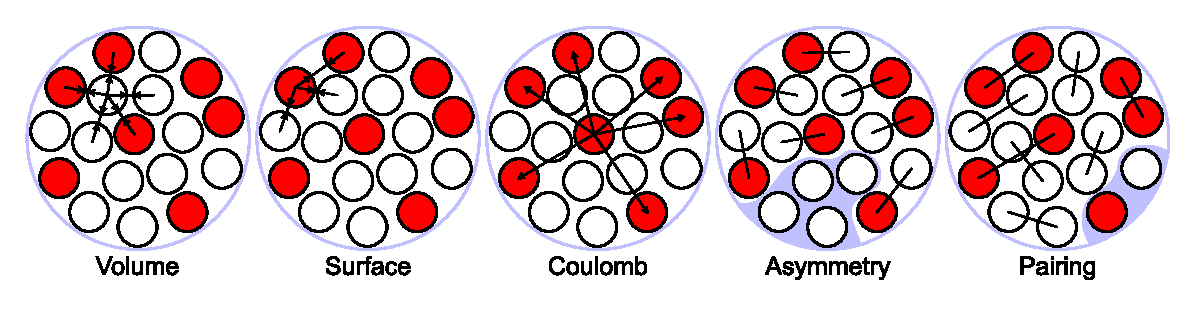
\includegraphics{figs/liquid-drop-model}
	\caption{Rappresentazione grafica del significato fisico dei termini presenti nel nuclear liquid drop model.}
	\label{fig:liquid-drop-model}
\end{figure}

Il suddetto modello ha base \textbf{fenomenologica}; la sola ipotesi
dell'andamento a corto raggio della forza non è sufficiente a
giustificare l'andamento reale

Come accennato, l'energia di legame tende ad assumere rapidamente il
valore medio di circa \(8MeV\) per nucleone (saturazione) il che indica
una energia di legame del nucleo proporzionale al numero di nucleoni
\begin{equation}
	\frac{B}{A} \simeq 8 MeV \qquad B \simeq 8 MeV \times A
    \label{eq:saturation-binding-energy-per-nucleon}
\end{equation}
Ora, se la forza nucleare si comportasse come una forza a lungo
raggio (come le forze gravitazionali o elettromagnetiche) ogni nucleone
interagirebbe con tutti i rimanenti altri per cui dovremmo attenderci
una energia di legame del nucleo tendenzialmente \emph{proporzionale al numero
di coppie} di nucleoni e dunque quadratica in A
\[
	B \propto \frac{A(A-1)}{2} \propto A^{2} \qquad
\]
Poiché i dati sulla energia di legame escludono questo tipo di
comportamento, dobbiamo concludere che ogni nucleone del nucleo
interagisce solo con un numero di fisso di nucleoni vicini per cui
concludiamo che \textbf{l'interazione forte ha un raggio d'azione finito}
dell'ordine di grandezza delle dimensioni del nucleone stesso.

Tale conclusione è in perfetto accordo con i dati sulla sezione d'urto
di neutroni su nuclei analizzati in precedenza che indicavano un \textbf{volume
nucleare proporzionale al numero di nucleoni}, ovvero una densità
volumetrica di nucleoni uniforme sul volume nucleare, fatto spiegabile
solo postulando la esistenza di una forza d'interazione tra nucleoni a
corto raggio.

Il primo tentativo di superare questo limite consiste nell'introdurre un
termine, sulla base della (\ref{eq:saturation-binding-energy-per-nucleon})
\begin{equation}
	B = a_{v} A
   \label{eq:volume-term-drop-model}
\end{equation}
dove la costante \(a_{v}\) viene detta \textbf{termine di volume}.
\begin{marginfigure}
	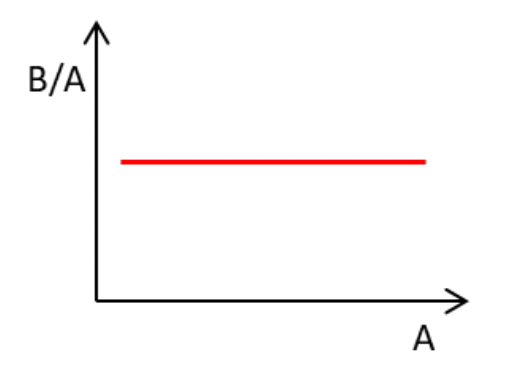
\includegraphics{figs/goccia1}
	%    \caption{This is a margin figure.}
	\label{fig:goccia1}
\end{marginfigure}
Con un tale andamento \(B / A\) , però, si finisce per ottenere una sovrastima
del volume.
La deviazione più rilevante si manifesta per valori piccoli di A dove
l'energia media di legame è molto inferiore a quanto previsto dalla
formula.
\bigskip

Si può allora osservare che, assumendo la forza nucleare a
corto raggio, si deve tenere conto che un nucleone prossimo alla
superficie del nucleo interagirà con un numero di nucleoni inferiore a
quello con cui interagirebbe qualora si trovasse all'interno del nucleo
stesso.
Ciò comporta che i nucleoni superficiali contribuiranno in
misura minore alla energia di legame nucleare di quelli interni al
volume.
Assumendo il nucleo di \textbf{forma sferica}, il numero di
nucleoni prossimi alla superficie sarà proporzionale a \(R^{2}\).
Dalla trattazione precedente (\ref{eq:nuclear-radius-skin}) sappiamo che (omettendo il termine di `skin'
nucleare) \begin{gather*}
	R_{\text{nuc}} = r_{0}A^{1/3}\\
	4 \pi R^{2} = 4 \pi (r_{0}A^{1/3})^2 \implies R_{\text{nuc}} \propto A^{2/3}
\end{gather*} per cui vi deve essere un termine che deve provocare un difetto di
energia di legame proporzionale ad \(A^{2/3}\): \[
	B = a_{v}A - a_{s}A^{2/3}
\] dove la costante \(a_{s}\) viene detta \textbf{termine di
	superficie}.
L'andamento di \(B / A\) con questa ulteriore correzione
può apprezzarsi a lato.
\begin{marginfigure}
	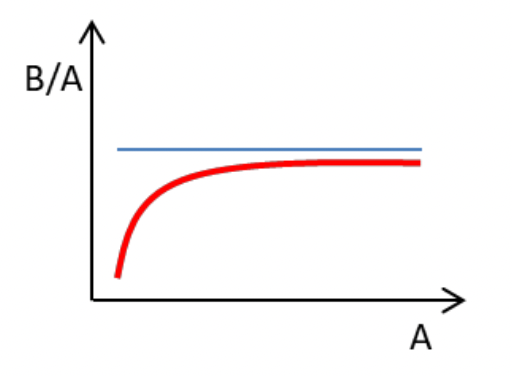
\includegraphics{figs/goccia2}
	%    \caption{This is a margin figure.}
	\label{fig:goccia2}
\end{marginfigure}
\bigskip

Un ulteriore miglioramento può essere ottenuto tenendo presente che i
protoni del nucleo si \emph{respingono elettrostaticamente} diminuendo
quindi il lavoro necessario per separarli dal nucleo stesso.
In effetti
se, per assurdo, si avesse un nucleo composto solo di protoni(senza
neutroni) il lavoro da spendere per mantenerne la configurazione sarebbe
sicuramente maggiore.

Ipotizzando una \emph{distribuzione di protoni uniforme} nel volume
nucleare (ricordiamo essere sferico dall'ipotesi precedente), otteniamo
la seguente espressione del lavoro fatto dalle forze coulombiane
repulsive per separare la carica nucleare
\begin{gather*}
	\delta L = \int _{R}^{\infty} \left( \frac{q \delta q}{4 \pi \epsilon_{0}r^{2}}  \hat{\bm{r}} \right)(dr \hat{\bm{r}})=
	- \frac{q \delta q}{4 \pi \epsilon_{0}r} \bigg |_{R}^{\infty} =
	- \frac{q \delta q}{4 \pi \epsilon_{0}R}\\
	q = \rho \frac{ 4}{3} \pi R^{3} \qquad \delta q = \rho 4 \pi R^{2} dR\\
	\delta L = \frac{1}{4 \pi \epsilon_{0}R}\left( \rho \frac{ 4}{3}\pi R^{3} \right)(\rho 4 \pi R^{2} dR) = \frac{4 \pi \rho^{2}}{3 \epsilon_{0}}R^{4}dR\\
	L = \int \delta l = \frac{4 \pi \rho^{2}}{15 \epsilon_{0}}R_{0}^{5} \qquad Q = \rho \frac{ 4}{3} \pi R_{0}^{3} = Ze\\
	L = \frac{3}{20 \pi \epsilon_{0}} \frac{Q^{2}}{R_{0}} = \frac{3e^{2}}{20 \pi \epsilon_{0}r_{0}} \frac{Z^{2}}{A^{1/3}}
	\implies L \propto \frac{ Z^{2}}{A^{1/3}}
\end{gather*} Ne consegue che la energia di legame nucleare dovrà essere corretta
sottraendo un termine proporzionale a \(Z^{2} / A^{1/3}\) per cui
l'espressione dell'energia di legame acquisirà la forma seguente
\begin{equation}
	B = a_{v}A - a_{s}A^{2/3} - a_{c} \frac{Z^{2}}{A^{1/3}}
	\label{eq:coulomb-term-drop-model}
\end{equation}
 dove la nuova costante \(a_{c}\) viene detta \textbf{termine
	coulombiano}.
Il termine coulombiano deve chiaramente annullarsi per
\(A=1\)(non c'e interazione elettrostatica) per cui l'unica forma
possibile è \[
	L \propto \frac{Z(Z-1)}{A^{1/3}} \quad
\]
\begin{marginfigure}
	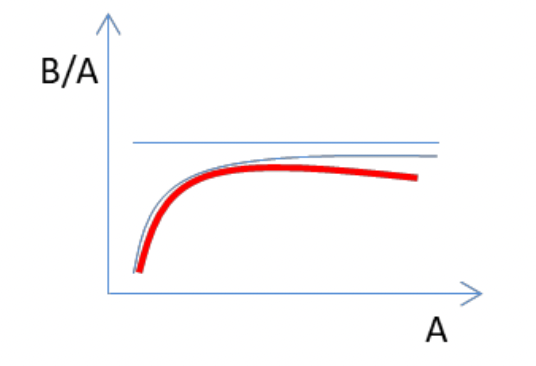
\includegraphics{figs/goccia3}
	%    \caption{This is a margin figure.}
	\label{fig:goccia3}
\end{marginfigure}

L'andamento $B / A$ risulta ulteriormente migliorato (si tenga presente
che nei nuclei stabili si ha approssimativamente \(Z=A/2\) per cui il
termine coulombiano sottrae un contributo crescente con \(A^{5/3}\)).

Se il modellino fenomenologico costruito finora fosse completo dovremmo
concludere che i nuclei più stabili(\(B= B_{max}\)) sono quelli con
\(Z=0\) ovvero i nuclei di soli neutroni.
Tale fatto è palesemente
contraddetto dai dati sperimentali i quali mostrano che i nuclei stabili
hanno un numero di protoni di poco inferiore a quello dei neutroni (la
differenza tra neutroni e protoni tende a crescere con il numero
atomico).
Il nostro modello -- basato sulla natura a corto raggio della
interazione nucleare -- non offre alcun appiglio per dare un fondamento
fisico a questo stato di cose che potrà essere spiegato solo nel
contesto della meccanica quantistica attraverso il \emph{principio di
	esclusione di Pauli}.
In questa situazione l'unica possibilità è quella
di introdurre un termine `ad hoc' capace di descrivere i dati
sperimentali.

Bisogna quindi fare in modo che il modello ci dica che i nuclei piu
stabili sono quelli con lo stesso numero di protoni e neutroni.
Raggiungiamo l'obiettivo introducendo un nuovo termine del tipo:
\[
	Z \simeq \frac{A}{2} \quad A - 2Z \simeq 0
\]
Ricordando però che con il crescere di \(A, Z\) tende ad essere via
via più piccolo di \(A/2\) (il quoziente protoni/neutroni diminuisce con
\(A\)), tale termine correttivo dovrà seguire una legge inversa ad A
modulata da un qualche esponente.
I dati indicano che la prima potenza è
sufficiente per cui abbiamo la seguente espressione della energia di
legame nucleare
\[
	B = a_{v}A - a_{s}A^{2/3} - a_{c} \frac{Z(Z-1)}{A^{1/3}} - \frac{a_{a}(A-2Z)^{2}}{A}
\]
dove la nuova costante \(a_{a}\) viene detta \textbf{termine di asimmetria}.
Notiamo che la presenza di \(A\) a denominatore è
giustificata osservando l'andamento dei dati sperimentali nel grafico
visto in precedenza:tanto piu \(A\) è grande tanto piu \(B / A\) devia
dalla tangente alla curva (quindi verso il basso).

Per completare il modello è necessario tenere conto di un ulteriore
proprietà dei nuclei.
I dati sperimentali mostrano che tra i 254 nuclei
stabili noti ben 148 sono del tipo \textbf{pari-pari} (un numero pari
sia di protoni che di neutroni), 101 sono del tipo \textbf{pari-dispari}
(un numero pari di protoni ma dispari di neutroni o viceversa) e solo 5
sono del tipo dispari-dispari (riportati in tabella \ref{tab:odd-odd-stable-nuclei}).
\begin{table}
	\centering
	\begin{tabular}{|c|}
		\hline
		$\isotope[2][1]{\mathlarger{H}}$ \\ \hline
		$\isotope[6][3]{\mathlarger{Li}}$ \\ \hline
		$\isotope[10][5]{\mathlarger{B}}$ \\ \hline
		$\isotope[14][7]{\mathlarger{N}}$ \\ \hline
		$\isotope[180m][73]{\mathlarger{Ta}}$ \\ \hline
	\end{tabular}
	\caption{Tabella dei nuclei stabili con both $ A,Z$ dispari.}
	\label{tab:odd-odd-stable-nuclei}
\end{table}

Similmente, tra i 35 nuclei a lunga vita media si hanno 22 pari-pari, 9 pari-dispari e 4
dispari-dispari.

Tali dati sembrano suggerire che per qualche motivo la forza forte tra
nucleoni da luogo a nuclei di maggiore stabilità quando vengono legati
\textbf{numeri pari} di neutroni e protoni, un fatto che trova una sua
diretta evidenza nell'andamento della energia di legame per nucleone
della serie isotopica dello xenon in Figura~\ref{fig:binding-energy-xenon}.
Tali dati sembrano suggerire che per qualche motivo la forza forte tra nucleoni da luogo a nuclei di maggiore stabilità
quando vengono legati \textbf{numeri pari} di neutroni e protoni, un fatto che trova una sua diretta evidenza nell’andamento della energia di legame per nucleone della serie isotopica dello xenon.
\begin{marginfigure}
	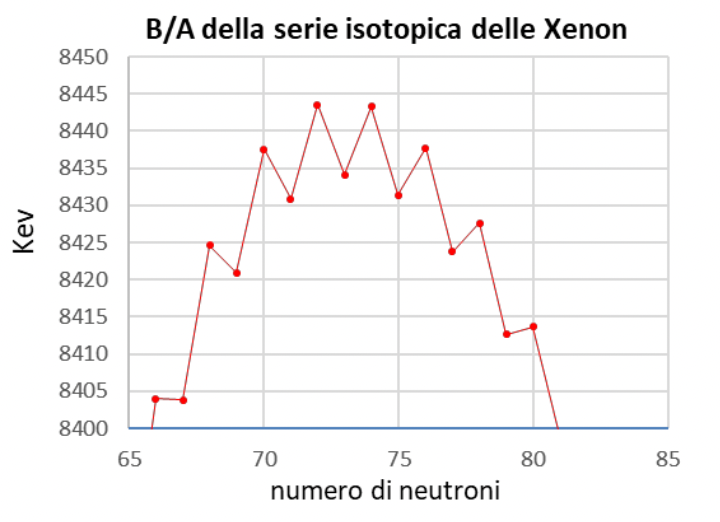
\includegraphics[scale = 1.5]{figs/goccia5}
	\caption{Andamento dell'energia di legame per la serie isotopica dello Xenon.}
	\label{fig:binding-energy-xenon}
\end{marginfigure}
Tenendo presente che il nucleo di Xenon ha \(Z=54\) protoni, si può
infatti constatare che gli isotopi con un numero pari di neutroni hanno
una maggiore energia di legame per nucleone.
Per rendere conto di questo
fatto si introduce un nuovo coefficiente detto di \textbf{pairing} \[
	a_{p} \frac{\delta}{A^{3/4}}
\] con \[
	\delta =
	\begin{cases}
		+1    \qquad  \text{pari-pari}       \\
		\ 0  \qquad  \ \ \text{pari-dispari} \\
		-1  \qquad  \text{dispari-dispari}
	\end{cases}
\] Giungiamo così alla seguente espressione complessiva della energia di
legame nucleare detta anche \textbf{formula semiempirica della energia
	di legame nucleare} o \textbf{formula di Weizsacker} della energia di
legame nucleare
\begin{equation}
	\boxed{    B = a_{v}A - a_{s}A^{2/3} - a_{c} \frac{Z(Z-1)}{A^{1/3}} - a_{a}\frac{(A-2Z)^{2}}{A} +     a_{p} \frac{\delta}{A^{3/4}}}
	\label{eq:weizsacker-formula}
\end{equation} Essa dipende da 5 parametri(vedi Fig.~\ref{fig:liquid-drop-model}) il cui valore numerico
viene determinato adattando la formula ai dati sperimentali di \(B/A\).

A titolo di esempio, una possibile combinazione di valori è la seguente(i
valori sono in \(MeV\)):
\[
	a_{v} = 15.5 \quad a_{s} = 16.8 \quad a_{c} = 0.72 \quad a_{a} = 23.0 \quad a_{p} = 34.0
\]
La formula della energia di legame nucleare è utile - come strumento di
calcolo - perchè suggerisce una prima interpretazione del nucleo e delle
forze che lo tengono insieme.

Da essa deduciamo che le forze tra nucleoni devono essere \textbf{molto
	intense} ma a \textbf{short range} (proprietà di saturazione), producono
una distribuzione spaziale tendenzialmente uniforme di nucleoni e
conducono ad una espressione della energia di legame con termini di
volume e superficie in analogia con quanto accade per i liquidi, ragione
che giustifica il nome spesso usato di \textbf{modello nucleare a
	goccia}.

Il modello a gas di fermioni (giustificabile con considerazioni
quantomeccaniche )riesce a rendere conto del termine \(a_{a}\) mentre
fallisce per quello di pairing.
Vedremo che il modello a shell sarà
quello piu preciso.


\section{Richiami di meccanica quantistica}\label{richiami-di-meccanica-quantistica}

\subsection{Osservabili e valori di aspettazione}\label{sec:osservabili-e-valori-di-aspettazione}

I sistemi fisici microscopici in regime non relativistico sono descritti
dalla funzione d'onda \(\psi(\bm{r},t)\) che si assume descriva in modo
completo lo stato fisico della particella, ovvero dica tutto ciò che può
essere detto su di essa.
Il significato fisico della funzione d'onda è
definito dalla ipotesi di Born secondo la quale il \emph{modulo quadrato
	fornisce la densità di probabilità di localizzazione della particella
	nel punto} \(\bm{r}\) al tempo t a seguito della interazione con un
apparato di misura: \[
	| \psi(\bm{r},t)|^{2}dV
\] Tale ipotesi comporta la \textbf{condizione di normalizzazione},
ovvero che l'integrale del modulo quadrato della funzione d'onda sul
volume occupato dal sistema microscopico debba essere pari ad uno, e
stabilisce che in meccanica quantistica la \textbf{grandezza fisica
	osservabile} sia il modulo quadrato della funzione d'onda piuttosto che
la funzione d'onda stessa.

Si assume infine che l'evoluzione temporale della funzione d'onda sia
governata dalla equazione di Schrödinger \[
	i \hslash \frac{\partial}{\partial t} \psi = \hat{H} \psi \qquad \hat{H} = - \frac{\hslash^{2}}{2m} \nabla^{2} + V
\] Come possiamo arrivare al \textbf{valore di aspettazione} di
posizione e quantità di moto?
Calcolo del valore medio della posizione
di una particella.
Nel caso di un' onda piana: \[
	\psi(\bm{r},t) = \psi_{0} e^{ i/\hslash (\bm{p} \cdot \bm{r}-Et) }
\] se \(p\) ed \(E\) fossero sempre definiti avrei che tutte le
posizioni nel piano hanno la stessa probabilità di essere misurate.
Per
cui una misurazione ripetuta potrebbe portare ad un esito diverso della
posizione. \(\implies\)ragionamento in termini
statistici\(\implies\)posso solo conoscere il \textbf{valore medio}
della posizione. \[
	\bm{r} |\psi(\bm{r},t)|^{2}dV \qquad <\bm{r}> = \sum_{i}^{n} \frac{\bm{r}_{i}p_{i}}{\sum_{i}^{n}p_{i}}
\]

\begin{equation}
	<\bm{r}> = \frac{\iiint_{V} \bm{r} |\psi(\bm{r},t)|^{2}dV }{\iiint_{V}|\psi(\bm{r},t)|^{2}dV }
\end{equation} dove il denominatore è unitario dalla condizione di
normalizzazione.
A questo punto si ha, con \(\psi^*\) complesso
coniugato, \[
	<\bm{r}> = \iiint_{V} \psi^*(\bm{r},t)\bm{r}\psi(\bm{r},t)\,dV
\] ovvero la \emph{media delle posizioni corrisponde alla media del
	vettore posizione \(\bm{r}\) pesata dal modulo quadro della funzione
	d'onda.}

Meno immediato è comprendere come calcolare ad esempio la quantità di
moto della particella.
Ragionando ancora una volta in modo euristico
possiamo richiamare le espressioni, scritte nel capitolo precedente, per
una data componente di Fourier della funzione d'onda \[
	- i \hslash \psi(\bm{r},t) = \hat{P} \psi(\bm{r},t) = \bm{p} \psi(\bm{r},t) \qquad
	i \hslash \frac{\partial}{\partial t} \psi(\bm{r},t) = \hat{E}\psi(\bm{r},t)= E\psi(\bm{r},t)
\] Si vede che nel caso in cui la funzione d'onda abbia quantità di moto
ed energia definite (ovvero nel caso in cui la funzione d'onda coincida
con una data componente di Fourier) allora gli operatori a primo membro
estraggono da essa i corrispondenti valori ponendoli nella posizione di
autovalori ovvero di moltiplicatori.
In meccanica quantistica si assume
che tale fatto abbia valida generale:

\begin{quote}
	Se in uno stato quantomeccanico \(\psi\) un osservabile ha un valore
	definito \(o\) allora lo stato \(\psi\) è autostato del corrispondente
	operatore \(O\) con autovalore \(o\)(\(O \psi = o \psi\)).
\end{quote}

Proseguendo nel ragionamento, operando sulla prima delle equazioni
precedenti(prima moltiplicando per \(\psi^{*}\) e poi integrando ambo i
membri) si ha

\begin{gather*}
	- i \hslash \nabla \psi = \bm{p} \psi \implies
	\psi^{*}(-i \hslash \nabla) \psi = \bm{p} \psi^{*}\psi\\
	\iiint_{V} \psi^{*}(-i \hslash \nabla) \psi \, dV = \iiint_{V} \bm{p} \psi^{*}\psi \, dV = \bm{p}\\
\end{gather*} dove si è sfruttata la normalizzazione della funzione d'onda.
Si noti
che tale espressione, valida nel caso di una data componente di Fourier,
è strutturalmente analoga alla posizione media delle posizioni della
particella microscopica (\(33\)) valida invece in generale.
Non è
difficile mostrare che nel caso di un generico pacchetto d'onde il
valore medio della quantità di moto della particella continua ad essere
dato da questo integrale per cui scriveremo \[
	<\bm{p}> = \iiint_{V} \psi^{*}\hat{P}\psi \, dV = \iiint_{V} \psi^{*}(- i \hslash \nabla )\psi \, dV
\] Inoltre, essendo le grandezze fisiche espresse da numeri reali, gli
operatori associati alle variabili dinamiche dovranno essere
\textbf{hermitiani}.

Giungiamo allora a formulare uno degli assiomi della meccanica
quantistica nella seguente forma:

\begin{quote}
	Ad ogni grandezza fisica misurabile \(o\) (osservabile) di un dato
	sistema microscopico, risulta associato un operatore lineare complesso
	hermitiano \(O\).
	Il valore medio delle misure della osservabile \(o\)
	al tempo \(t\) in un certo stato quantomeccanico \(\psi(\bm{r},t)\) è
	dato dal seguente integrale detto valore di aspettazione \[
		\boxed{<o> = \iiint_{V} \psi^{*}(\bm{r},t)\hat{O}\psi(\bm{r},t) \, dV}
	\]
\end{quote}

Quanto detto rende evidente che, dato un sistema quantomeccanico, si
pone il problema fondamentale di individuare le grandezze fisiche
osservabili e di determinare le corrispondenti operatori associati.
La
fisica atomica, ma ancor più la fisica delle particelle, chiariscono che
un criterio generale non esiste e che sia le osservabili che le loro
espressioni operatoriali possono essere trovate solo fondandosi sui dati
sperimentali.\\
Ciò non toglie che si sia verificato che le espressioni operatoriali
delle variabili dinamiche classiche possano essere trovate (sia pure con
alcune limitazioni che per ora tralasciamo) attraverso una procedura,
detta \textbf{principio di corrispondenza} (che applicheremo al caso del
momento angolare), la quale però non può essere applicata nel caso di
variabili dinamiche che non abbiano un corrispondente classico.
In tali
casi l'unica guida rimangono i dati sperimentali ed il percorso può
essere lungo e tortuoso.

\subsection{Definizione ed indefinizione delle osservabili}\label{sec:definizione-ed-indefinizione-delle-osservabili}

Una volta compreso in che modo debbano calcolarsi le variabili dinamiche
di un sistema quantomeccanico è necessario accennare ad un delicato
problema già sullo sfondo di alcune nostre considerazioni.
Riprendiamo
l'esempio dell'onda piana prograssiva visto poco fa. \[
	\psi(\bm{r},t) = \psi_{0}e^{ i/\hslash (\bm{p}\cdot \bm{r}- \omega t)}
\] Con tutta evidenza tale espressione descrive una particella avente
quantità di moto ed energia definite ma posizione spaziale e temporale
completamente \textbf{indefinite}.
Infatti, fissato il tempo, le
superfici equifase dell'onda risultano essere piani perpendicolari al
vettore quantità di moto.
Ciò significa che il modulo quadrato della
funzione d'onda assumerà un valore uniforme sui punti di tali superfici
(in realtà nel caso di una singola componente di Fourier su tutti i
punti dello spazio).
A sua volta ciò significa che la particella potrà
essere localizzata con densità di probabilità uniforme su tutti i punti
della superficie di un piano perpendicolare alla quantità di moto che
equivale ad affermare che la posizione della particella è assolutamente
indefinita.

Un minimo di conoscenza delle proprietà delle onde riconosce in questo
fatto qualcosa di noto poiché sappiamo bene che \emph{una qualunque
	componente di Fourier di un'onda piana possiede vettore d'onda e
	pulsazione definite ma posizione spaziale e temporale assolutamente
	indefinite}.

Sappiamo anche che per avere onde con posizione spaziale e temporale
meglio definite é necessario sovrapporre componenti di Fourier di
diverso vettore d'onda e pulsazione andando a costituire i cosiddetti
pacchetti d'onde.\\
Infine dalla \textbf{fisica classica}\footnote{The general idea is
	present in~\emph{any system where there are plane waves}~A physically
	realizable wave is always in the form of a wave packet which is finite
	in extent. A wave packet is built up by superposing waves with
	definite wave number. By simple Fourier analysis, a highly localized
	packet will require a wide spread of wave vectors, whereas a packet
	with a large spacial extent can be composed of wave numbers quite
	close to a specific value} sappiamo che nei pacchetti d'onde valgono
le cosiddette \textbf{relazioni di indeterminazione} che esprimono
queste proprietà in forma quantitativa approssimata \[
	\Delta k_{x} \Delta x \simeq2 \pi \qquad \Delta \omega \Delta t \simeq2 \pi
\] dove, data una direzione x dello spazio, \(\Delta k_{x}\) e
\(\Delta \omega\) stimano la dispersione del vettore d'onda e della
pulsazione del pacchetto, mentre \(\Delta x\) e \(\Delta t\) ne stimano
la dispersione spaziale e temporale.

\begin{marginfigure}
	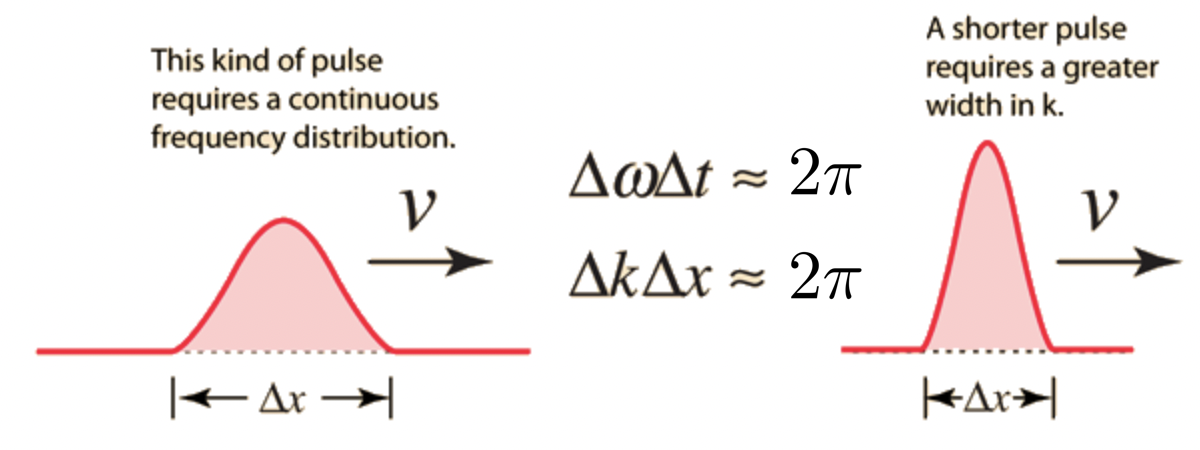
\includegraphics{figs/rel-indet}
	%    \caption{This is a margin figure.}
	\label{fig:rel-indet}
\end{marginfigure}

In generale si può dimostrare che valgono le seguenti relazioni \begin{gather*}
	\Delta k_{x} \Delta x \simeq2 \pi\\
	\Delta k_{y} \Delta y \simeq2 \pi\\
	\Delta k_{z} \Delta z \simeq2 \pi\\
	\Delta \omega \Delta t \simeq2 \pi\\
\end{gather*} Nel caso in cui si abbia un pacchetto d'onde che contenga solo una
componente di Fourier si avrebbe
\(\Delta k_{x} = \Delta k_{y} = \Delta k_{z} = 0\) con una conseguente
indeterminazione sulle posizioni tendente a \(\infty\).

Consideriamo il caso di un'onda piana,di lunghezza d'onda \(\lambda\) e
vettore d'onda \(\bm{k} = k_x \hat{\imath}\), che viene fatta passare
attraverso una fenditura ampia \(d\)(vedi figura).

\begin{marginfigure}
	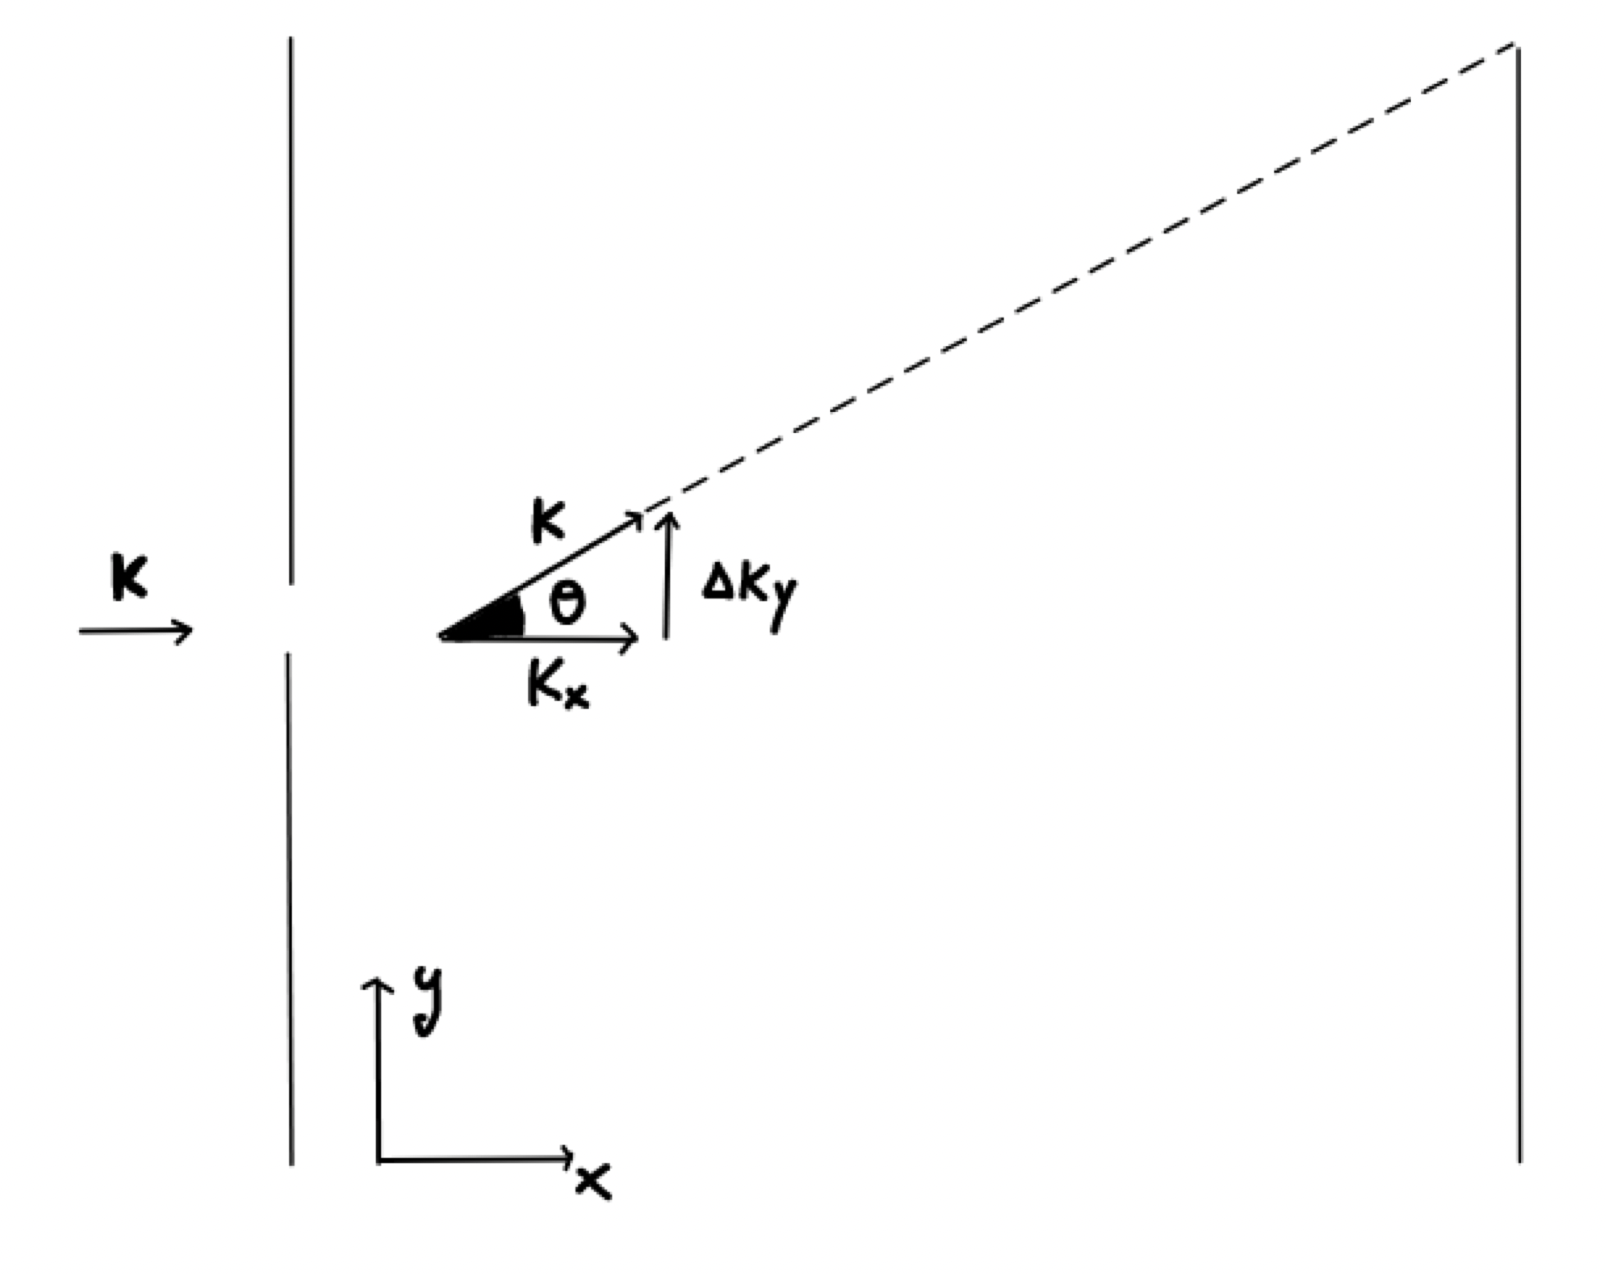
\includegraphics{figs/wave-electron-experiment}
	\caption{This is a margin figure.}
	\label{fig:wave-electron-experiment}
\end{marginfigure}

Il fronte d'onda viene tagliato dalla fenditura stessa:il fronte d'onda
lungo \(y\) ha un'incertezza \(\Delta y = d\).
Dalle relazioni
precedenti so che viene introdotto un errore
\(\Delta k_{y} \simeq\frac{2\pi}{d}\) .
La fenditura ha deviato il
vettore d'onda \(\bm{k}\) ed ora ha una certa angolazione \(\implies\)
il fronte d'onda che si incurva(dal Principio di Huygens-Fresnel).
L'angolo di apertura vale quindi \[
	\theta \simeq\frac{\Delta k_{y}}{k_{x}} \simeq \frac{2\pi}{d  \frac{2\pi}{\lambda}} \simeq\frac{\lambda}{d}
\] In ultima analisi quindi il fronte d'onda viene \textbf{limitato
	spazialmente} e dà luogo al fenomeno della \textbf{diffrazione}.

Vogliamo ora trovare l'analogo delle relazioni di indeterminazione in
\textbf{meccanica quantistica}.
Partiamo dalle relazioni \[
	\bm{p} = \hslash \bm{k} \qquad E = \hslash \omega \qquad p_{x} = \hslash k_{x}
\] e arriviamo a \begin{gather*}
	\Delta p_{x} \Delta x \simeq h\\
	\Delta p_{y} \Delta y \simeq h\\
	\Delta p_{z} \Delta z \simeq h\\
	\Delta E \Delta t \simeq h\\
\end{gather*} relazioni note come \textbf{relazioni di indeterminazione di
	Heisenberg} le quali affermano che

\begin{enumerate}
	\tightlist
	\item
	      se la misura della posizione di un corpuscolo materiale lungo una
	      certa direzione ha una incertezza \(\Delta x\) allora una simultanea
	      misura della quantità di moto lungo la stessa direzione ha una
	      incertezza \(\Delta p_x\) tale che il loro prodotto sia dell'ordine
	      della costante di Plank;
	\item
	      se la misura della posizione temporale di un corpuscolo materiale ha
	      una incertezza \(\Delta t\) allora una simultanea misura della energia
	      ha una incertezza \(\Delta E\) tale che il loro prodotto sia
	      dell'ordine della costante di Planck.
\end{enumerate}

Un analogo quantistico dell'esperimento precedente può consistere
nell'inviare un elettrone con quantità di moto
\(\bm{p} = p_{x} \hat{\imath}\) verso una fenditura di ampiezza \(d\).
Nel
momento in l'elettrone passa in mezzo alla fenditura possiamo
sicuramente dire che la sua posizione assume un qualche valore
\emph{all'interno del range} della fenditura.
Si ha quindi che il passaggio attraverso essa e la conseguente limitazione sulla posizione
della posizione \emph{equivale ad un'operazione di misura} sulla
particella.

\begin{marginfigure}
	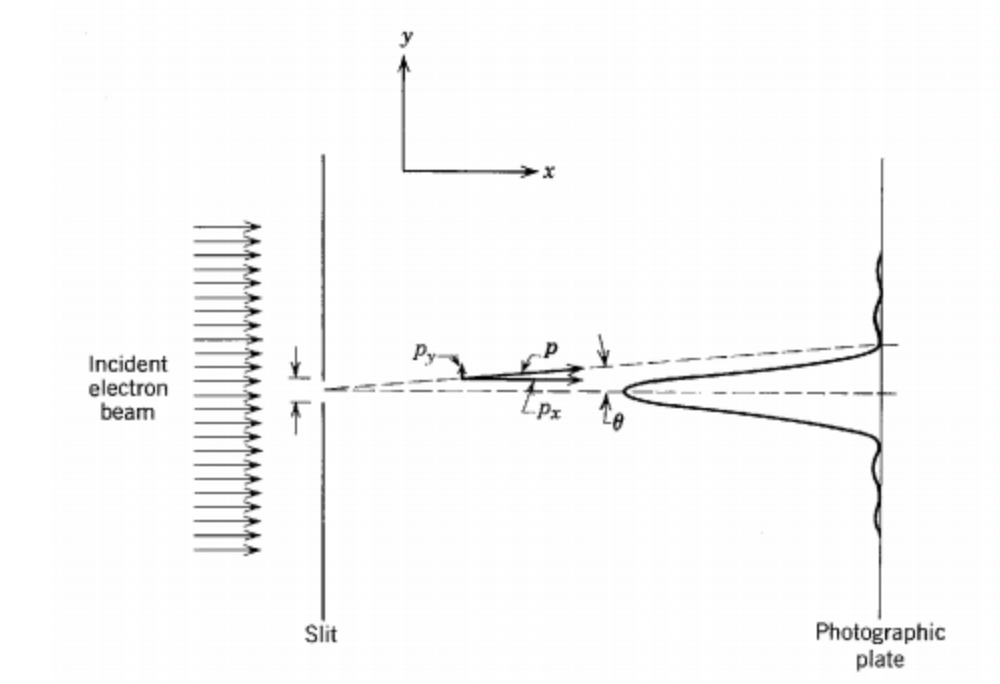
\includegraphics[width = 1.3 \textwidth, height = 1.3 \textheight]{figs/beam-electron-experiment}
	\caption{This is a margin figure.}
	\label{fig:beam-electron-experiment}
\end{marginfigure}

\[
	\Delta y \simeq d \qquad \Delta p_{y} \simeq \frac{h}{d}
\] con angolo di inclinazione
\[
	\theta \simeq \frac{\Delta p_{y}}{p_{x}} \simeq \frac{h}{d \frac{h}{\lambda}} \simeq \frac{\lambda}{d}
\]

L'incompatibilità tra le variabili dinamiche di un sistema
quantomeccanico è espressa in forma precisa da un fondamentale teorema
della meccanica quantistica il quale stabilisce che

\begin{quote}
	Il prodotto delle deviazioni standard delle misure di due grandezze
	fisiche \(a\) e \(b\) in uno stato \(\psi\) è limitato inferiormente dal
	valore di aspettazione del commutatore dei loro operatori diviso il
	fattore \(2i\)
	\begin{equation}
		\sigma_{a} \sigma_{b} \geq \iiint_{V} \psi^{*}(\bm{r},t) \frac{\hat{A}\hat{B} -\hat{B}\hat{A}}{2i} \psi(\bm{r},t) \, dV
	\end{equation}
\end{quote}

A titolo di esempio possiamo considerare proprio le variabili dinamiche
di posizione e quantità di moto\[
\] a = p\_\{x\} \qquad b = x \$\$

con corrispondente operatori \[
	- i \hslash \frac{\partial}{\partial x} \qquad x
\] e calcolarne il commutatore
\[
	\hat{X}\hat{P}_{x} - \hat{P}_{x}\hat{X}
\] per cui calcoliamo i due termini \begin{gather*}
	\hat{X}\hat{P}_{x} \psi = x \left(  - i \hslash \frac{\partial}{\partial x} \right) \psi = - i \hslash x \frac{\partial}{\partial x}\psi\\
	\hat{P}_{x}(\hat{X} \psi) = \left( - i \hslash \frac{\partial}{\partial x} \right)(x \psi)  = - i \hslash \left( \psi - x \frac{\partial}{\partial x} \psi \right) = - i \hslash \psi - i \hslash x \frac{\partial}{\partial x} \psi\\
\end{gather*} ed otteniamo \[
	(\hat{X}\hat{P}_{x} - \hat{P}_{x}\hat{X}) \psi = - i \hslash x \frac{\partial}{\partial x}\psi - \left[ - i \hslash \psi - i \hslash x \frac{\partial}{\partial x} \psi \right] = i \hslash \psi
\] da cui il valore del commutatore \[
	\hat{X}\hat{P}_{x} - \hat{P}_{x}\hat{X} = i \hslash  \hat{1}
\] che sostituito nella \((34)\) fornisce
\begin{gather*}
	\sigma_{x} \sigma_{p_{x}} \geq \iiint_{V} \psi^{*}(\bm{r},t) \frac{\hat{X}\hat{P}_{x} - \hat{P}_{x}\hat{X}}{2 i } \psi(\bm{r},t) \, dV =
	\iiint_{V} \psi^{*}(\bm{r},t) \frac{i \hslash  \hat{1}}{2i}\psi(\bm{r},t) \, dV\\
	\sigma_{x}\sigma_{p_{x}} \geq \frac{\hslash}{2}\\
\end{gather*} che esprime in forma rigorosa il principio di indeterminazione per le
misure della posizione e quantità di moto.

\subsection{Momento angolare orbitale}\label{sec:momento-angolare-orbitale}

Il momento angolare orbitale è un ottimo esempio per comprendere come si
possa utilizzare il \emph{principio di corrispondenza} per costruire
l'operatore quantomeccanico di una variabile dinamica a partire dalla
sua espressione classica
\[
	\bm{l}  = \bm{r} \wedge \bm{p}
\]
L'idea è quella di ottenere l'espressione quantomeccanica
dell'operatore associato attraverso la sostituzione diretta delle
variabili classiche con i corrispondenti operatori quantistici.
Richiamando allora gli operatori posizione e quantità di moto, otteniamo
la seguente espressione della terna ordinata di operatori che
costituiscono \textbf{l'operatore momento della quantità di moto}
\[
	\hat{L} = \hat{r} \wedge \hat{P}=\bm{r} \wedge (- i \hslash \nabla) = - i \hslash \ \bm{r} \wedge \nabla
\]
la quale, nel sistema di coordinate cartesiano, assume la seguente forma
\[
	\hat{L} = (\hat{L}_{x}, \hat{L}_{y}, \hat{L}_{z}) = - i \hslash \left( y \frac{\partial}{\partial z} - z \frac{\partial}{\partial y},z \frac{\partial}{\partial x}-x \frac{\partial}{\partial z}, x \frac{\partial}{\partial y} - y \frac{\partial}{\partial x} \right)
\] Dato che le proprietà generali di un operatore possono essere
studiate attraverso le sue relazioni di commutazione, utilizziamo la
foma cartesiana esplicita per calcolare i commutari della terna di
operatori.
Si ottiene facilmente
\[
	[\hat{L}_{x},\hat{L}_{y}] = i \hslash  \hat{L}_{z} \quad
	[\hat{L}_{z},\hat{L}_{x}] = i \hslash  \hat{L}_{y} \quad
	[\hat{L}_{y},\hat{L}_{z}] = i \hslash  \hat{L}_{x}
\]
Verifichiamo allora che uno stato quantomeccanico non ammette valori
definiti del momento della quantità di moto lungo \(x, y\) e \(z\)
poiché la proiezione lungo \(x\) è incompatibile con quella lungo \(y\),
quella lungo z con quella lungo \(x\) e quella lungo \(y\) con quella
lungo \(z\).
Ciò significa che \emph{in uno stato quantomeccanico il
	momento angolare può assumere valori definiti lungo una sola direzione}
che solitamente si assume come asse \(z\).

Consideriamo ora l'operatore \textbf{modulo quadrato del momento
	angolare} \[
	\hat{L}^{2} = \hat{L}_{x}^{2} + \hat{L}_{y}^{2} + \hat{L}_{z}^{2}
\] Sempre con calcolo diretto si ottengono facilmente i seguenti
commutatori \[
	\left[ \hat{L}^{2},\hat{L}_{x}\right] = \left[ \hat{L}^{2},\hat{L}_{y}\right] = \left[ \hat{L}^{2},\hat{L}_{z}\right] = 0
\]
\begin{marginfigure}
	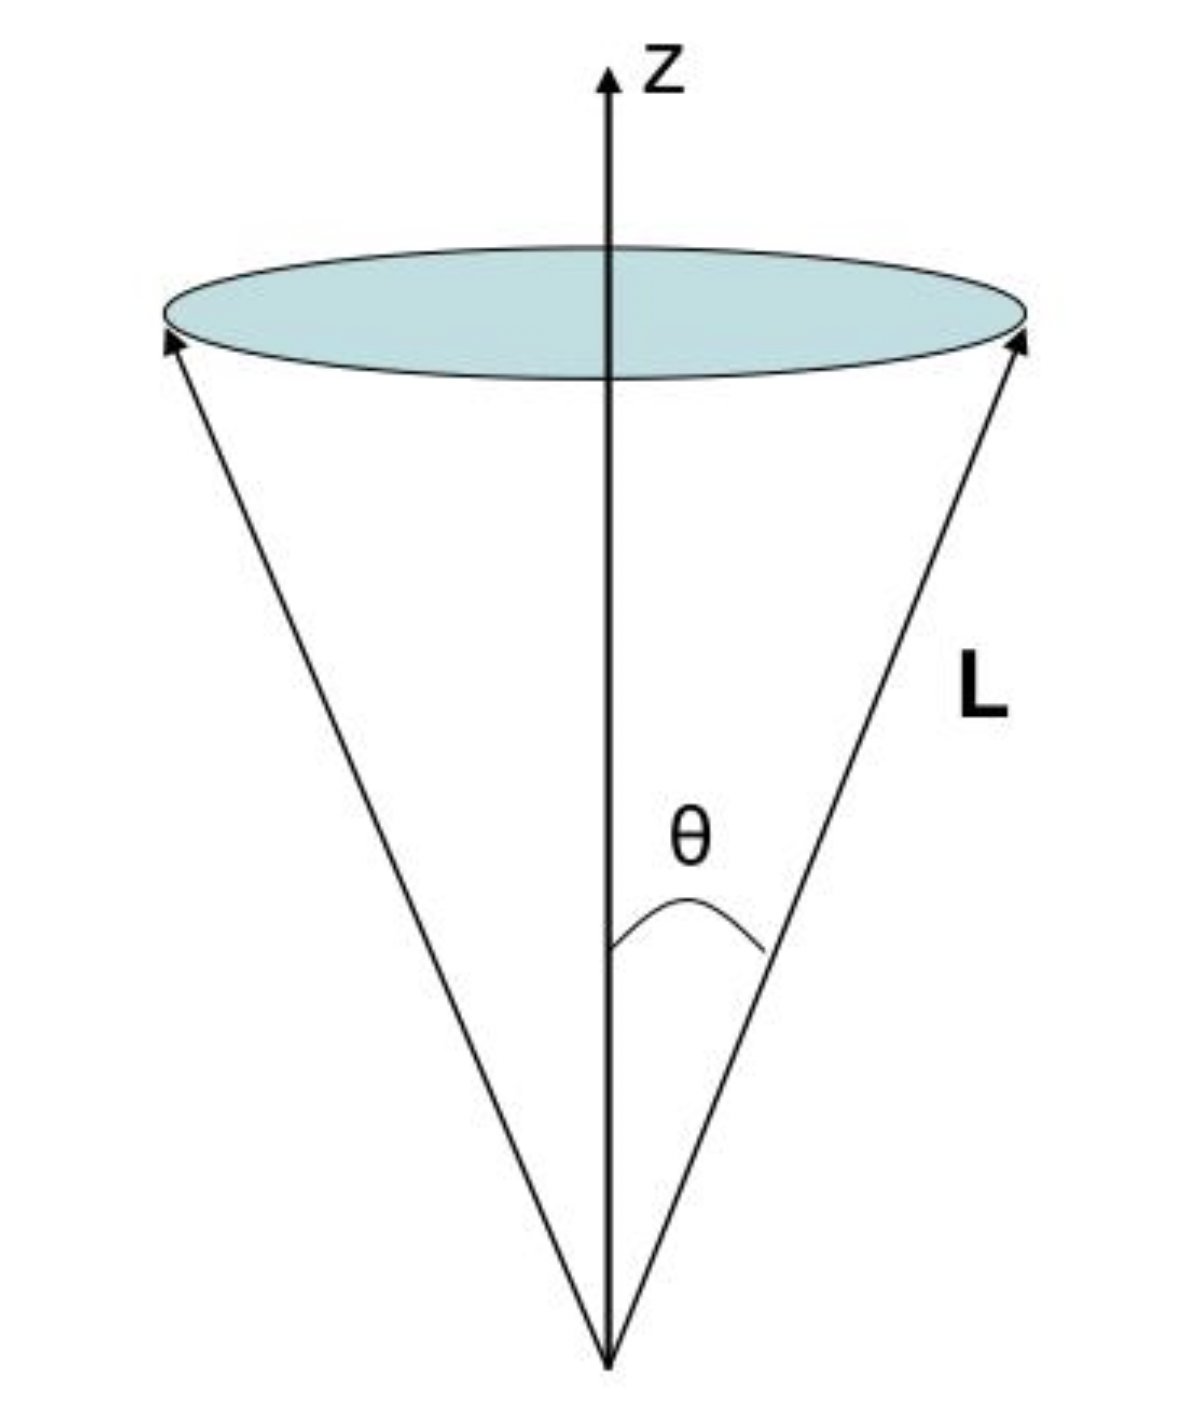
\includegraphics{figs/ang-mom-cone}
	\caption{Il set dei possibili valori di $\hat{L_x}$ e $\hat{L_y}$ descrive un cono attorno ad $\hat{L}_z$}
	\label{fig:ang-mom-cone}
\end{marginfigure}


Dalle relazioni di commutazioni scritte, concludiamo allora che
\textbf{uno stato quantomeccanico ammette valori definiti del quadrato
	del momento angolare e della sua componente lungo \(z\)}.

Giunti a questo punto si pone il problema di stabilire quali siano i
valori definiti del quadrato del momento angolare e della sua componente
lungo z e quali siano le espressioni della funzione d'onda dei
corrispondenti stati quantomeccanici.
Per rispondere a queste domande
occorre risolvere le equazioni agli autovalori degli operatori.
In
particolare, gli \textbf{autovalori forniranno i possibili valori del
	quadrato del momento angolare e della sua terza componente}, mentre le
corrispondenti \textbf{autofunzioni} forniranno le espressioni delle
\textbf{funzioni d'onda} degli stati quantomeccanici: \begin{gather*}
	\hat{L}^{2}\psi = \lambda \psi\\
	< \hat{L}^{2}> = \iiint_{V} \psi^{*} \hat{L}^{2}\psi \, dV = \lambda \iiint_{V} \psi \psi^{*} \, dV = \lambda\\
	\hat{L}^{2} \psi = \lambda' \psi \qquad  \hat{L}_{z} \psi = \lambda'' \psi\\
\end{gather*} Sviluppando il conto si ha \begin{gather*}
	\hat{L}^{2}\psi = l(l+1) \hslash^{2} \psi \qquad l = 0,1,2, \dots , n\\
	\hat{L}_{z} \psi = m \hslash \psi \qquad m = -l,-l + 1, \dots ,l-1, l\\
\end{gather*} Siamo difronte ad un operatore \textbf{quantizzato} ovvero che può
assumere valori \textbf{discreti}:i numeri interi l ed m descrivono
compiutamente lo stato quantomeccanico e vengono detti numeri quantici
del momento angolare.\\
\begin{marginfigure}
	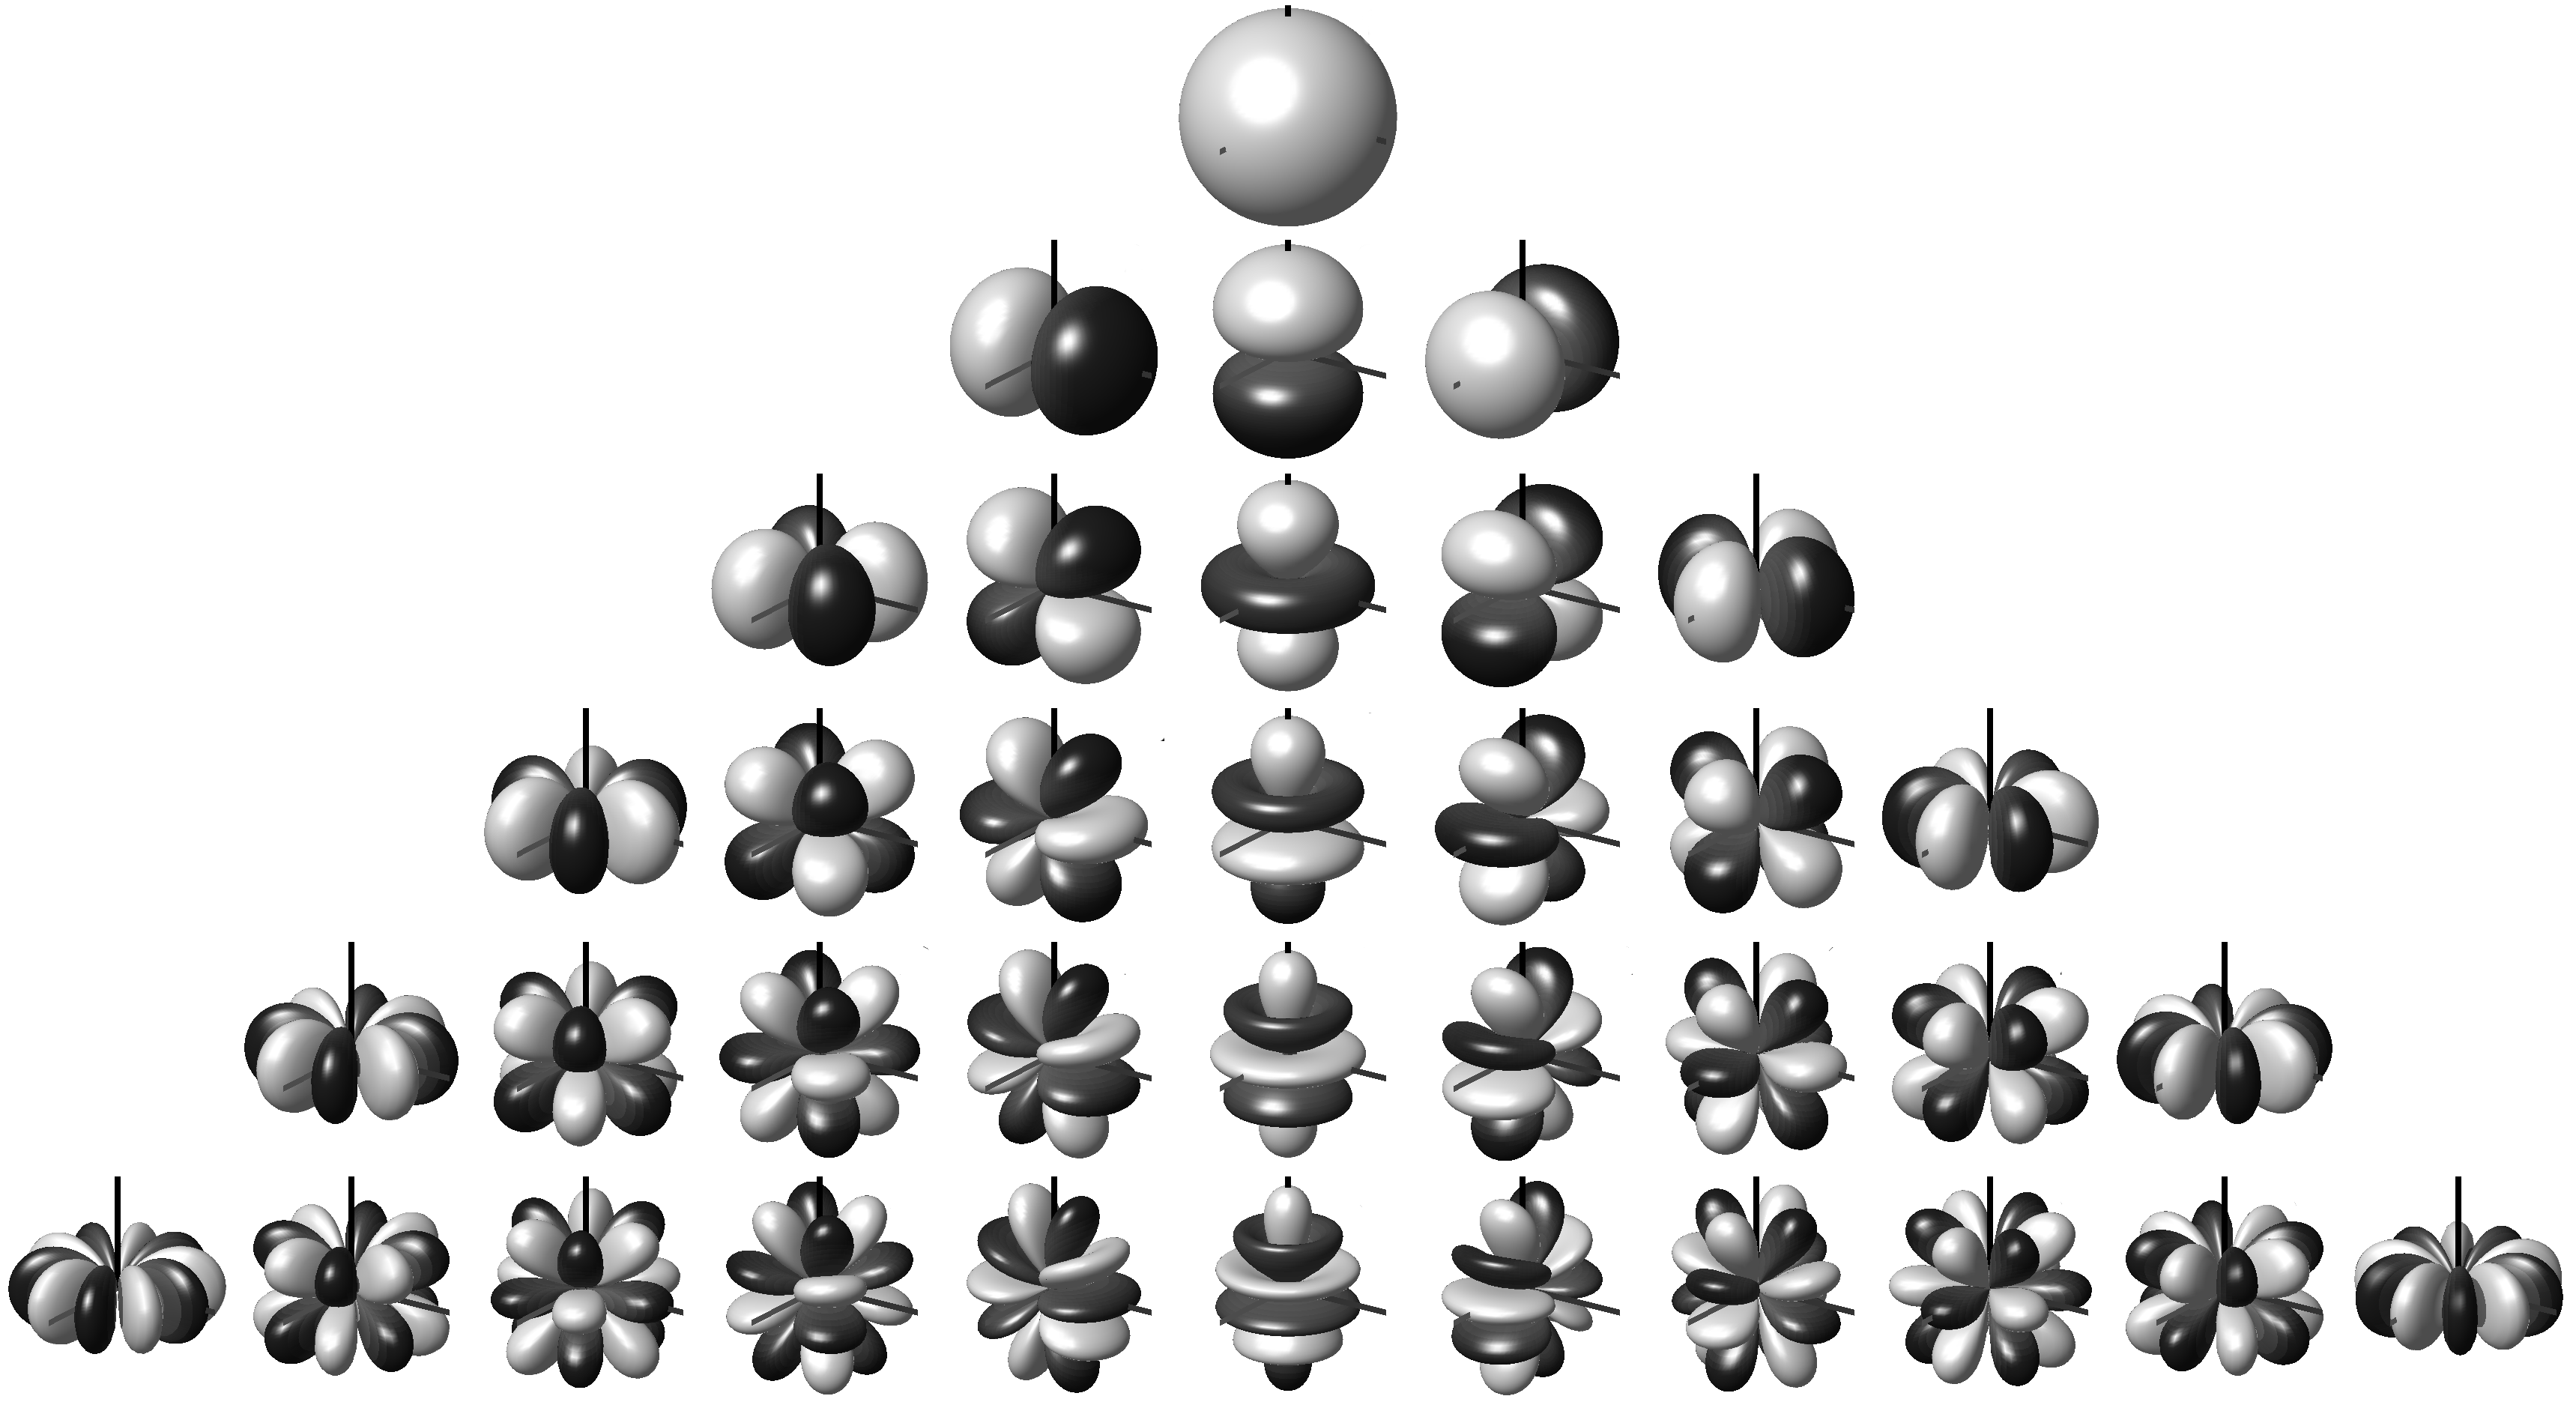
\includegraphics{figs/spherical-harmonics}
	\caption{Rappresentazione grafica delle prime armoniche sferiche.}
	\label{fig:spherical-harmonics}
\end{marginfigure}
In particolare le coppie di valori l ed m individuano spefiche funzioni
d'onda \(\psi_{l,m}(\theta,\phi)\) dette \textbf{armoniche sferiche}.
This peculiar set of functions comes out in the classical theory as well
when considering the modes of oscillation of a 2-dimensional membrane.

I possibili valori del quadrato del momento angolare sono dati dalla
successione discreta \(l(l+1) \hslash^{2}\) dove \(l=0,1,2 \dots\)
mentre i possibili valori del momento angolare lungo z sono dati dalla
successione discreta \(m \hslash\) dove
\(m = -l, -l + 1, \dots, l-1, l\) ovvero da una sequenza di \(2l+1\)
valori interi dipendente da \(l\).

\subsection{Momento angolare intrinseco o spin}\label{sec:momento-angolare-intrinseco-o-spin}

Nella meccanica classica i corpi materiali puntiformi possiedono al più
solo momento angolare orbitale mentre quelli estesi possono essere
portatori anche di un momento angolare intrinseco (spin).
Scegliendo il
polo di riduzione coincidente con il centro di massa del corpo
materiale, il momento angolare orbitale si annulla e l'unico momento
angolare residuo del corpo esteso è quello intrinseco che si manifesta
come rotazione del corpo stesso attorno ad un asse baricentrico.

Date queste premesse, ci si può domandare se anche le particelle
microscopiche possiedano un momento angolare intrinseco (spin) in
aggiunta al momento angolare orbitale.
I fatti sperimentali mostrano che
la risposta è affermativa e che il momento angolare intrinseco o spin
deve essere introdotto anche nel caso delle particelle microscopiche.
Vi
sono però delle sostanziali differenze

\begin{itemize}
	\tightlist
	\item
	      \textbf{meccanica classica}: un momento angolare intrinseco o residuo
	      può esistere solo per i \emph{corpi estesi} (non puntiformi) e questo
	      si interpreta come la somma dei momenti angolari orbitali di tutte le
	      parti che lo compongono;
	\item
	      \textbf{meccanica quantistica}: un momento angolare intrinseco o di
	      spin può esistere anche per le particelle puntiformi e come tale non è
	      riducibile in nessun modo a somme di momenti angolari orbitali delle
	      parti del sistema;
	\item
	      \textbf{meccanica classica}: il modulo del momento angolare intrinseco
	      può assumere con \emph{continuità qualunque valore}, ha un carattere
	      estrinseco e descrive essenzialmente lo stato cinematico di rotazione
	      del sistema rispetto ad un prefissato riferimento;
	\item
	      \textbf{meccanica quantistica}: il modulo del momento angolare
	      intrinseco può assumere un solo valore \emph{fisso} ed
	      \emph{immutabile}.
	      A seguito di tale invariabilità perde il suo
	      carattere estrinseco di natura cinematica ed assume - al pari della
	      massa e delle cariche interne del corpuscolo - lo status di grandezza
	      fisica intrinseca preposta alla descrizione di una nuova proprietà
	      statica della particella.
\end{itemize}

Per questi ed altri motivi possiamo affermare che \emph{lo spin è una
	variabile dinamica essenziamente quantistica} senza una diretta
corrispondenza classica.

Pauli pensò che fosse necessario introdurre una \textbf{terna di
	operatori di spin} \[
	S_{x} \qquad S_{y} \qquad S_{z}
\] soddisfacenti le regole di commutazione `tipo momento angolare' \[
	[ S_{x},S_{y}] = i \hslash S_{z} \qquad  [ S_{y},S_{z}] = i \hslash S_{x} \qquad   [ S_{z},S_{x}] = i \hslash S_{y}
\] ed operano sullo \textbf{spazio degli stati di spin}, uno `spazio
interno' diverso da quello su cui operano gli operatori del momento
angolare orbitale (lo spin è dunque un nuovo grado di libertà del
sistema microscopico).

In analogia con il caso del momento della quantità di moto, le regole di
commutazione appena scritte implicano che \textbf{uno stato
	quantomeccanico ammette valori definiti del modulo quadrato dello spin e
	e della sua terza componente}.

In particolare, risolta l'equazione agli autovalori degli operatori
quadrato del momento angolare di spin e della sua terza componente si
può ottenere l'insieme degli autovalori e delle autofunzioni: \begin{gather*}
	\hat{S}^{2} \eta_{s,s_{z}} = s (s+1) \hslash^{2} \eta_{s,s_{z}} \qquad s = 0, \frac{1}{2}, 1, \frac{3}{2}, \dots\\
	\hat{S}_{z} \eta_{s,s_{z}} = s_{z} \hslash \eta_{s,s_{z}} \qquad s_{z} = -s, -s+1, \dots , s-1, s\\
\end{gather*} dove \(s_{z}\) compie salti unitari tra un valore di \(s\) e il
seguente.
I possibili valori del quadrato del momento angolare di spin
sono dati dalla \(s(s+1)\hslash^{2}\).
Per ciascuno di questi, i
possibili valori del momento angolare di spin lungo \(z\) sono dati
dalla successione discreta di \(2s+1\) valori \(s_{z} \hslash\).
I
numeri \(s\) e \(s_{z}\) descrivono compiutamente lo stato
quantomeccanico e sono detti numeri quantici dello spin.
Essi
individuano specifici vettori \(\eta_{s,s_{z}}\) nello spazio degli spin
e dato che, fissato un certo \(s\) si hanno \(2s+1\) diversi valori di
\(s_{z}\) che individuano \(2s+1\) vettori linearmente indipendenti (e
normalizzati) nello spazio degli spin, ne deriva che \textbf{lo spazio
	dello spin di valore s è uno `spazio interno' complesso di \(2s+1\)
	dimensioni}.

Esempio: - Se \(s = \frac{1}{2}\) allora
\(s_{z} = - \frac{1}{2} , \frac{1}{2}\) ,
\(\eta_{\frac{1}{2},- \frac{1}{2}}, \eta_{\frac{1}{2}, \frac{1}{2}}\) -
Se \(s = 1\) allora \(s_{z} = -1,0,1\) ,
\(\eta_{1,1},\eta_{\frac{1}{2}, \frac{1}{2}}\) - Se \(s = 0\) allora
\(s_{z} = 0\) , \(\eta_{0,0}\) e si dice che la particella non ha spin

Da quanto detto consegue che lo stato quantomeccanico di una particella
microscopica di spin s dovrà essere rappresentato nello \emph{spazio
	prodotto} dello spazio degli stati quantomeccanici `ordinari' già visto,
con lo spazio degli stati di spin, ovvero dalla funzione d'onda `estesa'
\[
	\xi(\bm{r},t) =   \psi(\bm{r},t) \eta_{s,s_{z}}
\] dove \(\eta\) è il vettore di spin.

(È utile sta cosa?)L'analogo classico piu vicino all'onda piana,con
\(\eta_{\frac{1}{2}, \frac{1}{2}}\) ampiezza spinoriale, \[
	\eta_{\frac{1}{2}, \frac{1}{2}} \psi_{0}e^{ i/\hslash (\bm{p}\cdot \bm{r} - Et)}
\] è un'onda piana di campo elettrico \[
	\bm{E}_{0} \sin(\bm{k}\cdot \bm{r} - \omega t)
\]

E' importante sottolineare che l'introduzione di un apposito `spazio
complesso' per la descrizione degli stati di spin delle particelle
microscopiche costituisce un precedente teorico di grande rilevanza.
Essa infatti suggerisce che eventuali gradi di libertà interni delle
particelle richiesti dalla analisi dei dati sperimentali possano essere
descritti in ambito quantomeccanico semplicemente introducendo spazi
vettoriali complessi addizionali dotati della giusta dimensionalità.

\subsection{La somma dei momenti angolari}\label{sec:somma-dei-momenti-angolari}

Sia nei sistemi classici che quantomeccanici accade di dovere calcolare
il momento angolare di un sistema formato da due sottosistemi aventi
ciascuno un dato momento angolare, come si deve fare?

\begin{itemize}
	\tightlist
	\item
	      \emph{Fisica classica}: ai momenti angolari sono associati vettori,
	      pertanto al momento angolare del sistema complessivo si associa la
	      somma vettoriale dei momenti angolari dei due sottosistemi.
	      Dati
	      allora i momenti angolari \(\bm{J}_{1}\) e \(\bm{J}_{2}\) dei due
	      sottosistemi, il momento angolare del sistema complessivo sarà dato
	      dalla somma vettoriale \(\bm{J} = \bm{J}_{1}+ \bm{J}_{2}\) calcolata
	      con la regola del parallelogramma e dipendente da moduli direzioni e
	      versi relativi dei vettori sommati.
	      In particolare, il modulo di tale
	      momento angolare assumerà la seguente serie continua di valori \[
		      \bm{J} = \bm{J_{1}} + \bm{J_{2}} \qquad | |\bm{J_{1}}| - |\bm{J}_{2}| | \leq | \bm{J}| \leq|\bm{J}_{1} | | + | \bm{J}_{2} | |
	      \]
	\item
	      \emph{Meccanica quantistica}: ai momenti angolari sono associati
	      operatori, al momento angolare del sistema complessivo si associata
	      allora la somma operatoriale degli operatori momento angolare dei due
	      sottosistemi.
	      Dati allora gli operatori momento angolare
	      \(\hat{J}_{1}\) e \(\hat{J}_{2}\) dei due sottosistemi, l'operatore
	      momento angolare del sistema complessivo sarà dato dalla somma
	      operatoriale \(\hat{J} = \hat{J}_{1}+ \hat{J}_{2}\).
	      In accordo con le
	      regole generali della meccanica quantistica, si pone allora il
	      problema di determinare autovalori e autostati di tale operatore somma
	      dei momenti angolari.
\end{itemize}

In relazione a questo problema, è semplice mostrare con prova diretta
che se gli operatori \(\hat{J}_{1}\) e \(\hat{J}_{2}\) soddisfano le
relazioni di commutazione viste in precedenza allora anche l'operatore
\(\hat{J} = \hat{J}_{1}+ \hat{J}_{2}\) soddisferà relazioni di
commutazione dello stesso tipo.
Ciò significa che gli operatori
\(J^{2} = (J_{1} + \hat{J}_{2})^{2}\) e
\(\hat{J}_{z} = \hat{J_{1z}} + \hat{J_{2z}}\) avranno in generale i
seguenti autovalori \begin{gather*}
	j(j+1) \hslash^{2} \qquad j = 0, \frac{1}{2}, 1, \frac{3}{2}\\
	m \hslash  \qquad m = -j , -j +1, \dots , j-1, j\\
\end{gather*} Sulla base di considerazioni generali non è possibile dire di più,
per cui risulta necessario citare i risultati del teorema della somma
dei momenti angolari in meccanica quantistica.

Dati allora due stati quantomeccanici con momento angolare definito
\(\phi_{j_{1},m_{1}}\)e \(\phi_{j_{2},m_{2}}\) autostati degli operatori
\(\hat{J}_{1},\hat{J}_{1z}\) e \(\hat{J}_{2}, \hat{J}_{2z}\) si ha \begin{gather*}
	\hat{J}_{1}^{2} \ \phi_{j_{1},m_{1}}(\bm{r}) = j_{1}(j_{1}+1) \hslash \ \phi_{j_{1},m_{1}}(\bm{r}) \qquad j_{1} = 0, \frac{1}{2}, 1, \frac{3}{2}\\
	\hat{J}_{1z} \ \phi_{j_{1},m_{1}}(\bm{r}) = m \hslash \ \phi_{j_{1},m_{1}}(\bm{r})  \qquad m_{1} = -j_{1} , -j_{1} +1, \dots , j_{1}-1, j_{1}\\
	\hat{J}_{2}^{2} \ \phi_{j_{2},m_{2}}(\bm{r}) = j_{2}(j_{2}+1) \hslash \ \phi_{j_{2},m_{2}}(\bm{r}) \qquad j_{2} = 0, \frac{1}{2}, 1, \frac{3}{2}\\
	\hat{J}_{2z} \ \phi_{j_{2},m_{2}}(\bm{r}) = m \hslash \ \phi_{j_{2},m_{2}}(\bm{r})  \qquad m_{2} = -j_{2} , -j_{2} +1, \dots , j_{2}-1, j_{2}\\
\end{gather*} Lo stato quantomeccanico complessivo \(\phi_{j,m}\) è autostato degli
operatori \(J^{2} = (J_{1} + \hat{J}_{2})^{2}\) e
\(\hat{J}_{z} = \hat{J_{1z}} + \hat{J_{2z}}\) dove i loro numeri
quantici\(j\) ed \(m\) soddisfano le seguenti relazioni \begin{gather*}
	\hat{J}^{2} \ \phi_{j,m}(\bm{r}) = j(j+1) \hslash \ \phi_{j,m}(\bm{r}) \qquad | j_{1} - j_{2}|<j<|j_{1}+j_{2}|\\
	\hat{J}_{z} \ \phi_{j,m}(\bm{r}) = m \hslash \ \phi_{j,m}(\bm{r})  \qquad m = m_{1}+m_{2}\\
\end{gather*}

\emph{Esercizio didattico - Spazio di spinori 2 dimensionale}.
Consideriamo uno spazio di spinori identificato da \[
	s = \frac{1}{2} \qquad s_{z} = - \frac{1}{2} , \frac{1}{2}
\] per cui si hanno gli spinori \[
	\xi_{\frac{1}{2}, \frac{1}{2}} \qquad \xi_{- \frac{1}{2}, \frac{1}{2}}
\] Per quanto riguarda gli operatori di spin si ha \[
	\hat{S}^{2} \xi_{\frac{1}{2}, \pm \frac{1}{2}} = \frac{3}{4} \hslash^{2} \xi_{\frac{1}{2}, \pm \frac{1}{2}}
\] e \[
	\hat{S}_{z} \xi_{\frac{1}{2}, \frac{1}{2}} = \frac{1}{2} \hslash \xi_{\frac{1}{2}, \frac{1}{2}} \qquad
	\hat{S}_{z} \xi_{\frac{1}{2}, - \frac{1}{2}} = - \frac{1}{2} \hslash \xi_{\frac{1}{2}, -\frac{1}{2}}
\] Lo spazio è chiaramente bidimensionale dove le direzioni sono
identificate dai 2 spinori: {[}qui disegno di lato {]}

Nel momento in cui si utilizza uno spazio astratto per rappresentare lo
spin è necessario che valga la condizione della sovrapposizione di stati
che giustifica la spazializzazione dello spin.
A livello classico tale
richiesta in uno spazio ordinario sarebbe quella che tutte le posizioni
intermedie fossero accessibili.

In ogni caso siamo interessati solamente agli stati normalizzati, e
dunque non è fondamentale operare in tutto lo spazio, bensì possiamo
restringerci alla sfera unitaria.

Per dare una forma piu semplice e concreta agli spinori, eseguo la
seguente identificazione \[
	\xi_{\frac{1}{2}, \frac{1}{2}} =
	\begin{pmatrix}
		1 \\ 0
	\end{pmatrix} \qquad
	\xi_{\frac{1}{2}, - \frac{1}{2}} =
	\begin{pmatrix}
		0 \\ 1
	\end{pmatrix}
\] Gli operatori \(\hat{S}\) assumeranno forma matriciale in tale
rappresentazione \[
	S_{x,y,z} =
	\begin{pmatrix}
		\alpha & \alpha \\
		\alpha & \alpha
	\end{pmatrix}
\] Dovendo rispettare la condizione che \(S\) sia \emph{autoaggiunta} la
costruiamo come \[
	S_{x,y,z} =
	\begin{pmatrix}
		a      & b - ic \\
		b + ic & d
	\end{pmatrix}
\] Volendo però stare in totale generalità scriveremo

\begin{align*}
	S & =
	\begin{pmatrix}
		a + d & b-ic \\
		b+ic  & a-d
	\end{pmatrix} \\
	  & =
	a
	\begin{pmatrix}
		1 & 0 \\
		0 & 1
	\end{pmatrix}
	+ b \begin{pmatrix}
		    0 & 1 \\
		    1 & 0
	    \end{pmatrix}
	+ c \begin{pmatrix}
		    0 & -1 \\
		    1 & 0
	    \end{pmatrix}
	+d \begin{pmatrix}
		   1 & 0  \\
		   0 & -1
	   \end{pmatrix}
\end{align*}

Notiamo che qualunque matrice è combinazione lineare di queste 4
matrici\(\implies\) analogo dei versori.
Le matrici di base sono le
cossiddette \textbf{matrici di Pauli}. \[
	M = a \ I_{2 \times 2} + b \sigma_{1} + c \sigma_{2} + d \sigma_{3}
\] Osserviamo che la matrice identità non puo far parte in questa base,
altrimenti si andrebbe a perdere la condizione di non commutazione
propria degli operatori di spin(essa commuta con tutte le matrici).
La
rappresentazione matriciale di \(\hat{S}_{z}\) sarà la seguente \[
	\hat{S}_{z} \begin{pmatrix}
		1 \\
		0
	\end{pmatrix} =
	\frac{1}{2} \hslash \ I
	\begin{pmatrix}
		1 \\
		0
	\end{pmatrix}
	\qquad
	\hat{S}_{z} \begin{pmatrix}
		0 \\
		1
	\end{pmatrix}
	= - \frac{1}{2} \hslash I \begin{pmatrix}
		0 \\
		1
	\end{pmatrix}
\] \[
	\implies
	\hat{S}_{z} =
	\begin{pmatrix}
		\frac{1}{2} \hslash & 0                     \\
		0                   & - \frac{1}{2} \hslash
	\end{pmatrix}
\] Quindi \(\hat{S}_{z}\) deve essere \textbf{diagonale con i valori di
	spin sulla diagonale}.
Quindi quella appena scritta e una base
ortonormale (essendo gia i vettori normalizzati) di \(\hat{S}_{z}\)
\[
	\hat{S}_{z} = \frac{\hslash}{2}
	\begin{pmatrix}
		1 & 0  \\
		0 & -1
	\end{pmatrix} = \frac{\hslash}{2} \sigma_{3}
\] Svolgendo il conto vediamo che anche la relazione di commutazione
\[
	[ \hat{S}_{z}, \hat{S}_{x}] = i \hslash \hat{S}_{y}
\]
è rispettata.In conclusione
\[
	\hat{S}_{x} = \frac{\hslash}{2} \sigma_{1} \qquad
	\hat{S}_{y} =  \frac{\hslash}{2} \sigma_{2} \qquad
	\hat{S}_{z} = \frac{\hslash}{2} \sigma_{3}
\] Un vettore generico di spin generico si scrive come
\[
	\psi = \psi (\bm{r},t)
	\begin{pmatrix}
		\alpha \\
		\beta
	\end{pmatrix}
\]
Scelta una base ortonormale verifichiamo che
\[
	\hat{S}^{2}
	\begin{pmatrix}
		1 \\
		0
	\end{pmatrix}
	= (\hat{S}_{x}^{2} + \hat{S}_{y}^{2}+\hat{S}_{z}^{2})\begin{pmatrix}
		1 \\
		0
	\end{pmatrix} = \frac{3 \hslash^{2}}{4} I = \frac{3\hslash^{2}}{4} \begin{pmatrix}
		1 & 0 \\
		0 & 1
	\end{pmatrix}\begin{pmatrix}
		1 \\
		0
	\end{pmatrix}
	= 3 \frac{\hslash^{2}}{4} \begin{pmatrix}
		1 \\
		0
	\end{pmatrix}
\] risultato che ci aspettavamo.
Un aspetto piuttosto rilevante è che
abbiamo visto che \(\hat{S}\) ed \(\hat{S}_{z}\) sono gli unici
operatori a poter essere diagonalizzati contemporaneamente \(\implies\)
torna con l'interpretazione fisica sulla misurazione quantistica.

Si noti che, contrariamente al caso classico dove la somma di due
momenti angolari definiti fornisce un momento angolare definito, nel
caso quantistico ciò accade solo per la terza componente rimanendo
invece indefinito il suo modulo quadrato e dunque il numero quantico
\(j\).
Si tratta con tutta evidenza di una conseguenza delle
indefinizioni delle componenti \(x\) e \(y\) dei momenti angolari
sommati che rende però necessario precisare la relazione esistente tra
gli stati quantomeccanici dei sistemi parziali \(\phi_{j_1, m_1}\) e
\(\phi_{j_2,m_2}\) e lo stato quantomeccanico del sistema complessivo
\(\phi_{j,m}\).

In base a quanto detto precedentemente, dati \[
	(j_{1},m_{1}) \qquad (j_{2},m_{2})
\] Il teorema dice che \(j,m\) continuano ad essere interi e vale la
seguente relazione \begin{gather*}
	| j_{1} - j_{2}| \leq j \leq | j_{1} + j_{2} |\\
	m = m_{1} + m_{2}\\
\end{gather*} Mentre i sistemi parziali hanno momento angolare \begin{gather*}
	Y_{2,2}=(2,0) \qquad Y_{1,1}=(1,1)\\
	j = 1,2,3, \dots \quad m = 1\\
\end{gather*} il sistema totale non ha momento angolare definito\(\implies\)
collasso.
Vale la sovrappposizione \[
	a Y_{1,1}+bY_{2,1}+cY_{3,1}
\] dove \(a,b,c\) si dicono i \textbf{coefficienti di Clebsch-Gordan}.
In generale si può mostrare che \[
	\phi_{j_{1}m_{1}} \phi_{j_{2}m_{2}} = \sum_{\substack{j=| j_{1}-j_{2}| \\ m = m_{1}+m_{2}} }^{| j_{1}+j_{2}|} C_{jm}^{j_{1}m_{1}j_{2}m_{2}} \phi_{jm}
\]
\begin{marginfigure}
	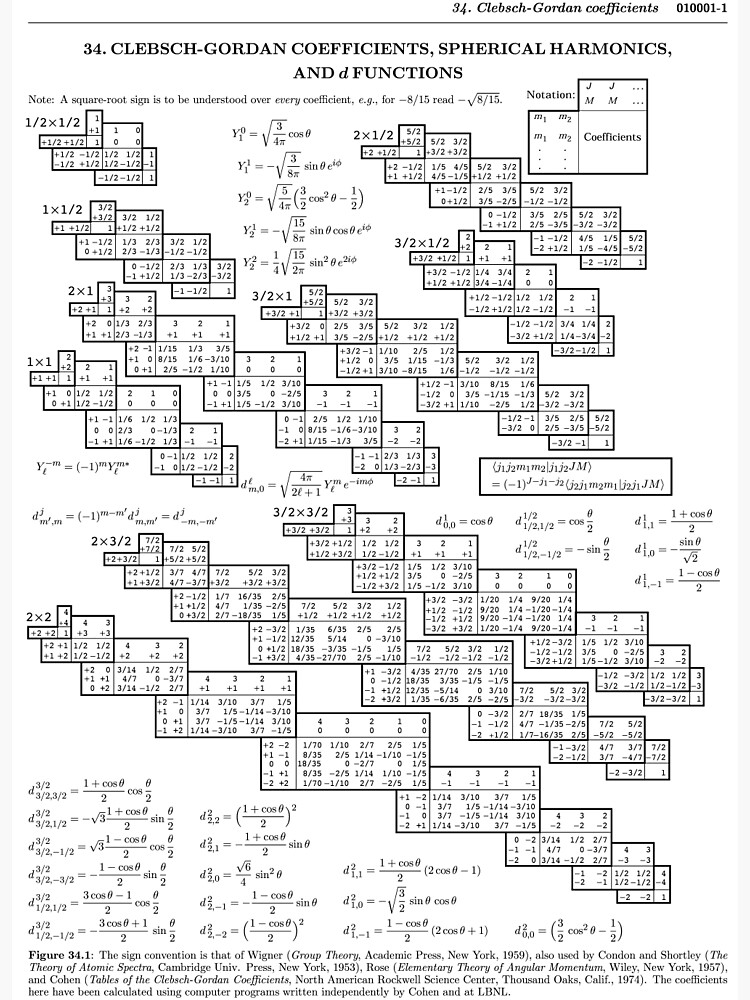
\includegraphics{figs/cl-gord}
	%    \caption{This is a margin figure.}
	\label{fig:cl-gord}
\end{marginfigure}
In figura a lato si può vedere una tabella di coefficienti di
Clebsch-Gordan.

\subsection{Stati quantomeccanici di due particelle identiche}\label{sec:particelle-identiche}

Lo studio dei sistemi quantomeccanici formati da particelle identiche conduce a nuove
sorprendenti proprietà che non trovano alcuna analogia nella fisica
classica.
Vediamo un esempio.

Immaginiamo di essere in ambito macroscopico e quindi soggetti alle
leggi della \emph{fisica classica}.
\begin{marginfigure}
	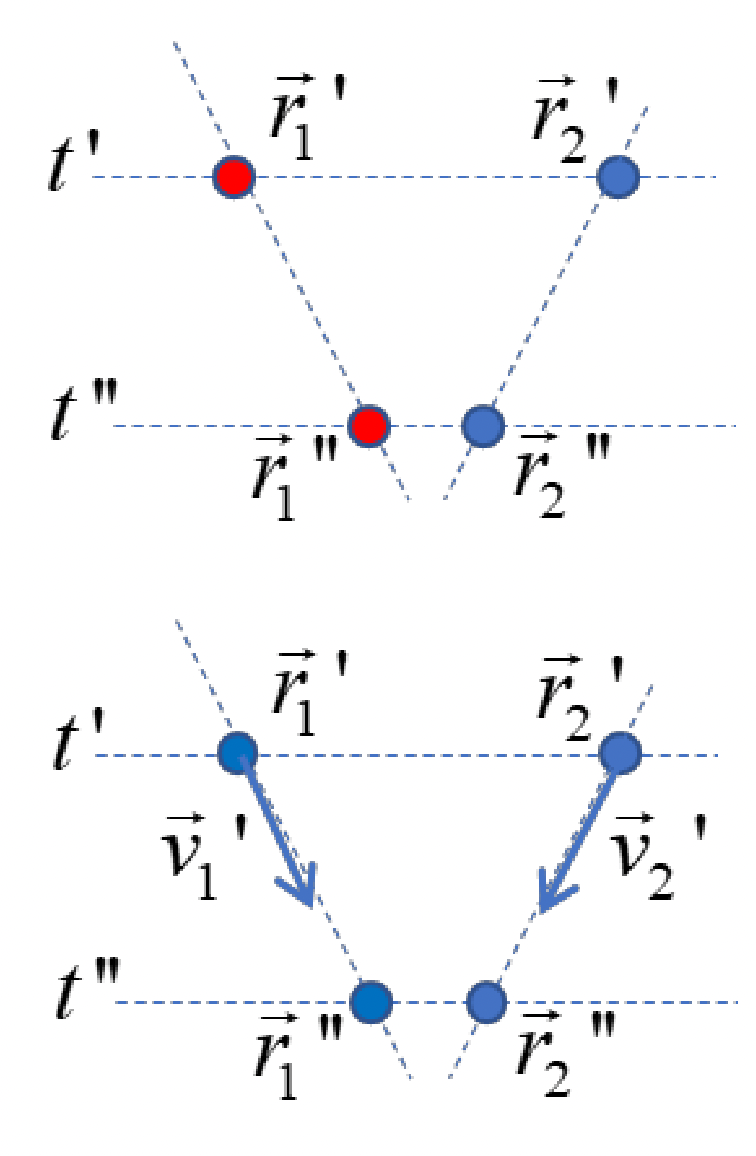
\includegraphics{figs/identical-part1}
	%    \caption{This is a margin figure.}
	\label{fig:identical-part1}
\end{marginfigure}
Immaginiamo poi che, in una certa porzione di spazio, si muovano due
piccole sferette, e che tale spazio sia illuminato ad intervalli di
tempo regolari da una luce stroboscopica.
Il lampo luminoso al tempo
\(t'\) mostrerà le due sferette nelle posizioni \(r_{1}'\) e \(r_{2}'\)
e quello al tempo \(t''\) in \(r_{1}''\) e \(r_{2}''\).
Con tutta
evidenza, se le due sferette sono diverse non esiste alcun problema
nell'associare alle posizioni osservate, in ogni dato istante di tempo,
la specifica sferetta.
Si dice allora che in meccanica classica due
particelle diverse sono sempre distinguibili.

Diverso sembra il caso in cui le due sferette siano identiche.
Infatti,
non sapremmo dire se la sferetta nella posizione \(r_{1}''(r_{2}'')\) al
tempo \(t''\) sia quella che al tempo \(t'\) si trovava in \(r_{1}'\) o
quella che si trovava in \(r_{2}'\).
L'identità delle sferette ci ha
condotti dunque alla impossibilità di associare con certezza le
posizioni alle particelle.
L'ambiguità, però, non è essenziale poichè
può essere superata qualora al tempo t' siano note, non solo le
posizioni delle sferette, ma anche le loro velocità \(v_1'\) e \(v_2'\).
Infatti, al tempo \(t''\) ciascuna sferetta dovrà trovarsi non troppo
lontano dalla direzione della propria velocità al tempo \(t'\) (se
l'istante \(t''\) non è troppo lontano da \(t'\)).
Concludiamo allora
che, se in un istante di tempo le posizioni e le velocità di due
sferette identiche sono note con sufficiente precisione, sarà sempre
possibile determinare la loro posizione in ogni istante di tempo
successivo.

Poiché nella meccanica classica non ci sono limitazioni nel conoscere in
ogni istante di tempo le posizioni e le velocità delle particelle in
gioco, concludiamo che \textbf{nella fisica classica sia le particelle
	diverse che quelle identiche sono sempre distinguibili}.

Cosa accade in meccanica quantistica?
E' semplice rendersi conto che nel
caso di particelle diverse una ipotetica misura di massa, carica o di
una qualunque variabile interna capace di determinarne l'identità sarà
in grado di dirci senza ambiguità quale posizione occupi ciascuna delle
due particelle.
Dunque, analogamente al caso della meccanica classica,
giungiamo quindi ad affermare che nella meccanica quantistica due
particelle diverse sono sempre distinguibili.

Ben diverso è il caso in cui le particelle siano identiche.
Infatti - a
differenza di ciò che accade in meccanica classica -- uno stato
quantomeccanico non può possedere in ogni istate di tempo sia posizioni
definite che velocità definite (principio di indeterminazione).
Se ad
esempio al tempo \(t'\) sono definite le posizioni \(r_{1}'\) e
\(r_{2}'\) delle due particelle identiche, risulteranno allora
indefinite le corrispondenti velocità \(v_{1}'\) e \(v_{2}'\)
pregiudicando dunque la possibilità di attribuire univocamente una
posizione a ciascuna di esse al tempo t'\,. Analogamente, se al tempo
t' sono definite le velocità \(v_{1}'\) e \(v_{2}'\) delle due
particelle identiche (e dunque le quantità di moto), risulteranno allora
indefinite le loro posizioni che non potranno essere univocamente
assegnate alle particelle stesse.

Giungiamo allora a concludere che \textbf{nella meccanica quantistica
	due particelle identiche sono sempre indistinguibili}.
Tale fatto può
essere visto in modo ancor più diretto attraverso il seguente\\
esempio.
Immaginiamo di avere due particelle microscopiche identiche che
si trovino in stati quantomeccanici diversi, ad esempio di quantità di
moto ed energia (\(E_1, p_1\)) ed (\(E_2, p_2\)) descritte da due onde
piane di De Broglie (vedi figura).\\
\begin{marginfigure}
	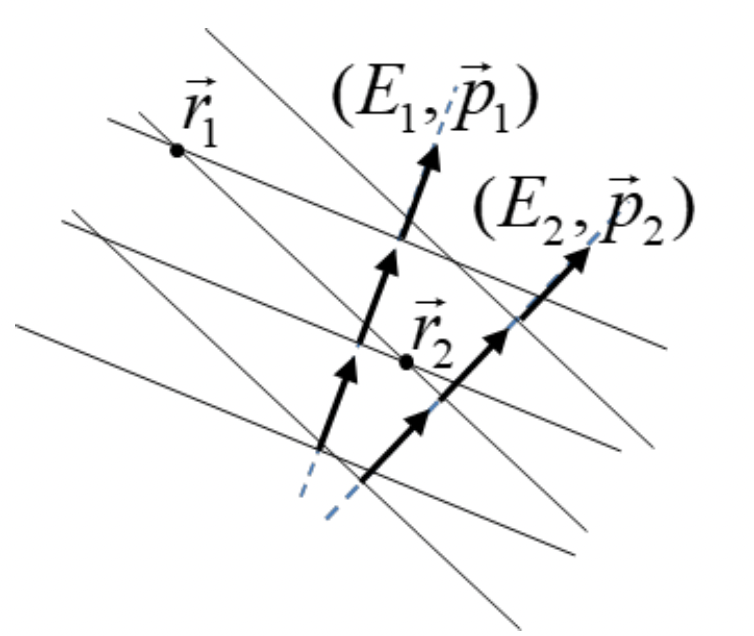
\includegraphics{figs/identical-part2}
	%    \caption{This is a margin figure.}
	\label{fig:identical-part2}
\end{marginfigure}
Con tutta evidenza due misure di posizione potranno trovare la
particella (\(E_{1},p_{1}\)) nella posizione \(r_{1}\) e la particella
(\(E_{2},p_{2}\)) nella posizione \(r_{2}\), oppure la particella
(\(E_{2}, p_{2}\)) nella posizione \(r_{1}\) e la particella
(\(E_{1}, p_{1}\)) nella posizione \(r_{2}\), dando quindi luogo alla
ambiguità discussa.

L'esempio può guidarci anche alla costruzione della funzione d'onda del
sistema quantomeccanico delle due particelle identiche.\\
Per cominciare consideriamo due particelle identiche poste in regioni di
spazio differenti ovvero mutuamente isolate (ad esempio ponendole in
contenitori diversi).
La densità di probabilità di osservare la
particella (\(E_{1},p_{1}\)) nella posizione \(r_{1}\) e la particella
(\(E_{2},p_{2}\)) nella posizione \(r_{2}\) è data allora dal modulo
quadrato della seguente funzione d'onda

\begin{equation}
	\psi_{E_{1},\mathbf{p}_{1}}(\mathbf{r}_{1},t) \psi_{E_{2},\mathbf{p}_{2}}(\mathbf{r}_{2},t)
\end{equation}

dove i termini a prodotto sono le funzioni d'onda delle singole
particelle \begin{gather*}
	\psi_{E_{1},\mathbf{p}_{1}}(\mathbf{r}_{1},t) = A_{E_{1},\mathbf{p}_{1}}e^{ \frac{i}{\hbar} (\mathbf{p}_{1} \cdot \mathbf{r}_{1}-E_{1}t)}\\
	\psi_{E_{2},\mathbf{p}_{2}}(\mathbf{r}_{2},t) = A_{E_{2},\mathbf{p}_{2}}e^{ \frac{i}{\hbar} (\mathbf{p}_{2} \cdot \mathbf{r}_{2}-E_{2}t)}\\
\end{gather*} Se ora rimuoviamo la condizione di isolamento, costruendo un unico
sistema fisico formato da due particelle identiche poste nella stessa
regione di spazio (ad esempio mettendole entrambe nello stesso
contenitore) ci rendiamo subito conto che la funzione d'onda (\(35\))
non descrive lo stato quantomeccanico in modo completo.
Infatti - come
osservato in precedenza -- è anche possibile che una misura di posizione
sul sistema trovi la particella (\(E_{2},p_{2}\)) in \(r_{1}\) e la
particella (\(E_{1},p_{1}\)) in \(r_{2}\), un esito evidentemente non
descritto dalla (\(35\)).
Tale esito è invece descritto dalla seguente
funzione d'onda

\begin{equation}
	\psi_{E_{2},\mathbf{p}_{2}}(\mathbf{r}_{1},t) \psi_{E_{1},\mathbf{p}_{1}}(\mathbf{r}_{2},t)
\end{equation} dove i termini a prodotto sono dati dalle funzioni d'onda
delle singole particelle

\begin{gather*}
	\psi_{E_{1},\mathbf{p}_{1}}(\mathbf{r}_{2},t) = A_{E_{1},\mathbf{p}_{1}}e^{ \frac{i}{\hbar} (\mathbf{p}_{1} \cdot \mathbf{r}_{2}-E_{1}t)}\\
	\psi_{E_{2},\mathbf{p}_{2}}(\mathbf{r}_{1},t) = A_{E_{2},\mathbf{p}_{2}}e^{ \frac{i}{\hbar} (\mathbf{p}_{2} \cdot \mathbf{r}_{1}-E_{2}t)}\\
\end{gather*}
Ora, dato che il sistema di due particelle identiche può dare luogo
ad entrambi gli esiti (\(35\)) e (\(36\)), tali esiti -- in accordo con
i principi generali della meccanica quantistica - dovranno essere
sommati coerentemente.
In assenza di ulteriori prescrizioni, non potremo
che introdurre due generici coefficienti complessi ottenendo uno stato
che - pur soddisfacendo i requisiti richiesti - contiene due
coefficienti arbitrari
\[
	\psi_{sis} = \alpha \, \psi_{E_{1},\mathbf{p}_{1}}(\mathbf{r}_{1},t) \psi_{E_{2},\mathbf{p}_{2}}(\mathbf{r}_{2},t) +
	\beta \, \psi_{E_{2},\mathbf{p}_{2}}(\mathbf{r}_{1},t) \psi_{E_{1},\mathbf{p}_{1}}(\mathbf{r}_{2},t)
\]
una ambiguità nota con il nome di \textbf{degenerazione di scambio}.

%%%%%%%%%%%%%%%%%%%%%%%%%%%%%%%%%%%%%%%%%%%%%%%%%%%%%%%%%%%%%%%%%%%%%%%%%%%%%%%%%%%%%%%%%%%%%%%%%%%%%%%%%%%%%%%%%%%%%%%%
%%%%%%%%%%%%%%%%%%%%%%%%%%%%%%%%%%%%%%%%%%%%%%%%%%%%%%%%%%%%%%%%%%%%%%%%%%%%%%%%%%%%%%%%%%%%%%%%%%%%%%%%%%%%%%%%%%%%%%%%
%%%%%%%%%%%%%%%%%%%%%%%%%%%%%%%%%%%%%%%%%%%%%%%%%%%%%%%%%%%%%%%%%%%%%%%%%%%%%%%%%%%%%%%%%%%%%%%%%%%%%%%%%%%%%%%%%%%%%%%%
\section{Il nucleo come gas di fermioni}\label{sec:il-nucleo-come-gas-di-fermioni}

Il modello a goccia del nucleo - essenzialmente fondato sulla natura a corto raggio delle interazioni forti - riesce a
descrivere alcune proprietà del nucleo tra le quali l’esistenza di una energia di legame con termini di volume, superficie e coulombiano.
Non riesce invece a rendere conto in nessun modo dei termini di asimmetria e accoppiamento, chiaramente richiesti dai
dati sperimentali, ma che devono essere introdotti ‘a mano’ nella formula di Weizsacker.
Tale fatto dimostra che oltre alla natura a corto raggio delle interazioni forti, nel nucleo giocano un ruolo di rilievo
altre proprietà trascurate dal modello a goccia, presumibilmente legate alla natura quantomeccanica dei suoi costituenti.
Il modello nucleare a gas di fermioni introduce nel gioco alcuni essenziali proprietà quantomeccaniche in una forma il
più possibile semplificata.






%%%%%%%%%%%%%%%%%%%%%%%%%%%%%%%%%%%%%%%%%%%%%%%%%%%%%%%%%%%%%%%%%%%%%
\appendix
\chapter{Appendice A : Integrazione sull'angolo solido della sezione d'urto di scattering}
\label{ch:integrazione-sezione-urto-angolo-solido}
 \begin{fullwidth}
    Integriamo la sezione d'urto di scattering sullo schermo $ S_O$ su cui si osserva la diffrazione in approssimazione di
    far field(schermo lontano).
    Supporremo inoltre lo schermo molto esteso rispetto all'estensione della figura di diffrazione.
    \[
        \sigma_{scatt} = \iint_{\Omega} |f(\bm{q})|^2 \, d \Omega = \iint_{S_O} \frac{|f(\bm{q})|^2}{r^2} \, da
    \]
    Ora, sostituendo l'espressione della scattering amplitude (\ref{eq:scattering-amplitude}) ed utilizzando l'identità
    $ |f|^2 = \bar{f}f$ abbiamo
    \begin{align}
        \sigma_{scatt} &= \iint_{S_O} \left[
            \frac{1}{{r}^{2}} \left(
            \frac{ik}{2 \pi} \iint_{S_B} \Gamma(\bm{r}')
            e^{-i \bm{q} \cdot \bm{r}'} \, da'
            \right)
            \left( - \frac{ik}{2 \pi} \iint_{S_B} \bar{\Gamma}(\bm{r}') e^{i \bm{q} \cdot \bm{r}''} \, da'' \right)
            \right] \,  da  \nonumber \\
        & =  \frac{{k}^{2}}{4 \pi^2} \iint_{S_O} \left( \frac{1}{{r}^{2}} \iint_{S_B}  \iint_{S_B}
        \Gamma(\bm{r}') \bar{\Gamma}(\bm{r}'') e^{i \bm{q} \cdot (\bm{r}''-\bm{r}')} \, da'' da' \right) \, da \nonumber\\
        & = \frac{{k}^{2}}{4 \pi^2}  \iint_{S_B}  \iint_{S_B}\left(\iint_{S_O} \frac{1}{{r}^{2}}
        \Gamma(\bm{r}') \bar{\Gamma}(\bm{r}'') e^{i \bm{q} \cdot (\bm{r}''-\bm{r}')} \, da \right) \, da'' da'
        \label{eq:sigma-scattering-1}
    \end{align}
    Vogliamo ora sviluppare la fase dell'esponenziale.
    Assumendo un sistema di coordinate cartesiano con l’asse z orientato normalmente agli schermi, la coordinata z
    del secondo schermo assume valori grandi, si hanno allora le relazioni seguenti
    \[
    r = \sqrt{ x^{2}+y^{2}+z^{2} } = z \sqrt{ 1+ \frac{x^{2}+y^{2}}{z^{2}} } \simeq z \left( 1 + \frac{x^{2}+y^{2}}{2z^{2}} \right)
    = z + \frac{x^{2}+y^{2}}{2z} \simeq z
    \]
    Per quanto riguarda il vettore d'onda trasferito, definendo $\hat{ \bm{n}} = \frac{\bm{r}}{r}$ nell'approssimazione
    di $z \gg x,y$ si ha
    \begin{gather*}
        \bm{q} = k (\hat{\bm{n}} - \hat{\bm{n}}') = k \left( \frac{\bm{r}}{r}  - \hat{\bm{k}}\right) \simeq k\left( \frac{x}{z}\hat{\bm{i}} + \frac{y}{z} \hat{\bm{j}} + \hat{\bm{k}} -\hat{\bm{k}}\right) = k\left( \frac{x}{z} \hat{\bm{i}} +\frac{y}{z} \hat{\bm{j}} \right)\\
        \bm{q} \cdot (\bm{r}'' - \bm{r}'') \simeq \left( \frac{x}{z} \hat{\bm{i}} + \frac{y}{z} \hat{\bm{j}} \right) \cdot [(x''-x')\hat{\bm{i}} + (y''-y')\hat{\bm{j}}+(z''-z')\hat{\bm{k}}]
    = \frac{kx}{z}(x''-x') +\frac{ky}{z}(y''-y')
    \end{gather*}
    che sostituite nella (\ref{eq:sigma-scattering-1}) forniscono
    \[
    \sigma_{scatt} = \frac{k^{2}}{4 \pi^{2}} \iint_{S_{B}}\iint_{S_{B}} \left( \iint_{S_{O}} \frac{1}{z^{2}} \Gamma(\bm{r}')\bar{\Gamma}(\bm{r}'') e^{ i \frac{kx}{z}(x''-x') + i \frac{ky}{z} (y'' - y')} \, dxdy\right) da''da'
    \]
    Nelle nostre ipotesi $S_{o} \gg S_{B}$, per cui sviluppiamo la precedente come
    \[
     = \frac{k^{2}}{4 \pi^{2}} \iint_{S_{B}}\iint_{S_{B}} da'' da'\frac{1}{z^{2}} \Gamma(\bm{r}') \bar{\Gamma}(\bm{r}'') \frac{4 \pi^{2}z^{2}}{k^{2}}\left( \frac{1}{2 \pi} \int_{-\infty}^{\infty} e^{ ik \frac{x}{z}(x'-x'') } \frac{x}{z} \, dk  \right)\left( \frac{1}{2 \pi} \int_{-\infty}^{\infty} e^{ ik \frac{y}{z}(y'-y'') } \frac{y}{z} \, dk  \right)
    \]
    Utilizzando ora l'espressione esponenziale della delta di Dirac:
    \[
    \int_{-\infty}^{\infty} e^{ ikx } \, dk = 2 \pi \, \delta(x)
    \]
    riscriviamo
    \[
    \sigma_{scatt} = \iint_{S_{B}}\iint_{S_{B}} \Gamma(\bm{r}') \bar{\Gamma}(\bm{r}'') \delta(x''-x')\delta(y''-y') \,dx''dy''dx'dy'
    \]
    Tenendo ora conto di
    \begin{itemize}
        \item $z'' = z'$ avendo scelto il riferimento con l'asse $z$ normale al piano di integrazione;
        \item le delta di dirac bloccano gli integrali ai valori $x''=x',y''=y'$;
        \item $\bm{r}''=\bm{r}'$(gli assi $z$ e $z'$ sono collineari). %%%TODO 12/12/22 niccolozanotti: spiegare perche. Spiega bene il fatto che |f|^2 = fbar * f di stessa variabile --> poi
    \end{itemize}
    in defininita abbiamo
    \[
    \sigma_{scatt} = \iint_{S_{B}}  \Gamma(\bm{r}') \bar{\Gamma}(\bm{r}'') \, dx'dy'= \iint_{S_{B}} |\Gamma(\bm{r}')|^{2} \, dx'dy'
    \]
    Abbiamo quindi ritrovato la (\ref{eq:scattering-cross-section-profile-func}):
    \[
    \sigma_{scatt} = \iint_{S_{B}}  |\Gamma(\bm{r}')|^{2} \, da'
    \]
\end{fullwidth}


\chapter{Appendice B : Funzione di Bessel di ordine zero}
\label{ch:funzione-bessel-zero}
Appendice B

\chapter{Appendice C : Integrazione della funzione di Bessel di ordine zero}
\label{ch:integrazione-bessel-zero}
Appendice C


\mainmatter


\backmatter

%----------------------------------------------------------------------------------------
%	BIBLIOGRAPHY
%----------------------------------------------------------------------------------------

\bibliography{bibliography} % Use the bibliography.bib file for the bibliography
\bibliographystyle{plainnat} % Use the plainnat style of referencing

%----------------------------------------------------------------------------------------

%\printindex % Print the index at the very end of the document
%\bibliography
\end{document}